	\chapter{The LIGO Instrument}\label{LIGOInstrument}
	The previous chapter dealt with gravitational waves and briefly touched on how a laser interferometer is well suited for detecting GWs and in its simplest form, the LIGO instrument is an incredibly large Michaelson interferometer. However, to make a practical gravitational-wave observatory, the complexity will have to be extended far beyond what Michelson and Morley used.  The next sections will explore the various upgrades to the instrument configuration that improve the sensitivity of LIGO.
	
		\subsection{Simple Michaelson}\label{sec:michelson}
		As shown in Figure \ref{fig:simple_michelson}, the interferometer begins with a laser which is incident on a partially-reflecting and partially-transmitting beamsplitter that sends half of the laser light down each arm.  The individual beams gather phase as they propagate down the arms and then reflect off of two end mirrors and eventually recombine at the same beamsplitter.  Whether the light constructively or destructively interferes will depend on their relative accumulated phase from propagating down each arm. A photodetector is placed at the output and measures the total power which converts the total amount of light into an electronic signal.  In Section \ref{measuringGWs}, it was shown that the differential time of flight between photons traveling down the individual arms carry gravitational wave information.  
		The difference in flight times, $\Delta t$, can be converted into how much phase, $\Delta \phi$, is accumulated by the photons as they propagate through space.  
		
		But the question remains, how does an interferometer explicitly measure $\Delta \phi$?
		
		If the input electric field of the interferometer is $E_0$, the beamsplitter will transmit $iE_0 /\sqrt{2}$ down the x-arm and reflect $E_0 /\sqrt{2}$ towards the y-arm.  By setting the beamsplitter to be the origin, the two plane waves traveling down their respective arms will have gathered a phase $\phi_i$, where the individual arms are denoted by the subscripts. Then, upon reflecting off the end mirrors and returning to the beamsplitter the resultant fields are transmitted to the antisymmetric port. Each of the electric fields from the arms can be described by these equations
			\begin{equation}
			\begin{aligned}
				E_{x} 	&=	\frac{i E_0}{2} e^{2i\phi_{x}}	
			\\	E_{y} 	&=	\frac{i E_0}{2} e^{2i\phi_{y}}
			\end{aligned}
			\end{equation}
		Since the electromagnetic waves are linear, the resultant sum of waves at the antisymmetric port will be $E_{out} = E_x + E_y$. The photodiode at the output (or antisymmetric) port detects the integrated power which is related to the total electric field by
			\begin{equation}
			\begin{aligned}\label{asy_power}
				P_{AS}	&= \int_{\text{Area}} I \;				\text{d}A 
			\\			&= \int_{\text{Area}} \vert E_x + E_y \vert^2 \;	\text{d}A 
			\\			&= P_{in} \; \cos^2(\Delta \phi)
			\end{aligned}
			\end{equation}	
		where $\Delta \phi = \phi_{x} - \phi_{y} = k_x l_x - k_y l_y$ and $P_{in} = \int_{\text{Area}}	 \vert E_0\vert^2 \text{d}A$ is the input power. By using equation \ref{diffphase} and the common (or average) arm length $l_{+} = \frac{l_x + l_y}{2}$, the power due to a differential phase shift is
			\begin{equation}
			P_{AS}\vert_{\text{Bright}} \approx P_{in} \; (1-2 \Delta \phi) = P_{in} \; (1-2 k l_{+} h_{+})
			\end{equation}
		There is a large DC term that is dependent on the input power and generally, it is very difficult to measure small changes in a large signal.  This is configuration can be referred to as being on a bright fringe. So the next obvious method is to shift the arm lengths such that the output port is operating on a dark fringe, normally this is called a null-point operation.  However, there are difficulties associated with this method as well. Consider shifting the phase of equation \ref{asy_power} by $\pi/2$, which would result in
			\begin{equation}\label{null}
			P_{AS} \vert_{\text{Dark}} = P_{in} \; \text{sin}^2 (\Delta \phi) \approx P_{in} \; (k l_{+} h_{+})^2 
			\end{equation}
		This results in a second-order dependence on a gravitational-wave signal that is already approximated to be very small.  So a good solution to the issue of how to $read$ out a gravitational wave signal can be remedied using radio frequency (RF) detection methods. By changing the interferometer input from a single laser to adding an electro-optical modulator (EOM) that sinusoidally modulates the laser frequency and expanding to first order using the Bessel functions,
			\begin{equation}\label{modE}
			\begin{aligned}
			E_{in} 	&= E_{0} e^{i(wt + \beta \text{cos} (\Omega t))} \\
					&\approx E_0 e^{iwt} [J_0(\beta) + J_1(\beta) e^{i \Omega t} + J_1(\beta) e^{-i \Omega t}] \\
					&= E_{C,in} + E_{SB+,in} + E_{SB-,in}
			\end{aligned}
			\end{equation}
		where $\Omega$ and $\beta$ are the modulation frequency and depths, respectively. The first term is commonly called the carrier field whereas the second and third terms are referred to as the (upper or lower) sidebands.  Because there are multiple electric fields, it is useful to define an optical transfer function which maps the interferometer's input fields to its output,
		\begin{equation}\label{opt_tf}
		E_{out} = E_{C} + E_{SB+} + E_{SB-} = 
		\begin{pmatrix}
			t_{C} 	&   
		\\ 	t_{SB+} &
		\\ 	t_{SB-} &
		\end{pmatrix}
		\begin{pmatrix}
		E_{C,in} &    E_{SB+,in}    &  E_{SB-,in}     
		\end{pmatrix}
		\end{equation}
		The carrier transfer function, $t_{C}$ has already been calculated by equations \ref{asy_power} - \ref{null} and the sideband transfer functions are not much different.
		\begin{equation}\label{sb_tf}
		t_{SB\pm} = r_{x,\pm}  e^{i\phi_{\pm,x}} - r_{y,\pm}  e^{i\phi_{\pm,y}}
		\end{equation}
		where $\phi_{\pm,i} = (k \pm k_{\Omega}) \, \ell_{i} = (\frac{w+\Omega}{c} ) \ell_{i}$. In the current example, the sidebands and carrier fields reflect off the end mirrors identically, however, this will not be true in general when dealing with resonators that are highly frequency dependent.  Plugging equation \ref{sb_tf} into \ref{opt_tf}, the output electric field becomes 
		\begin{equation}
		E_{out} = i e^{iwt} [ J_0(\beta) 	k \ell_{+}  h_{+}  \; + \; J_1(\beta) \sin( k \Delta \ell + k_{\Omega} \Delta \ell) (e^{i\Omega t}  + e^{-i\Omega t}) ]
		\end{equation}
		where $\Delta \ell = \frac{l_x-l_y}{2}$ is the average differential arm length. The frequency offset of the sidebands allow them to accumulate phase differently than the carrier field. Thus, by choosing a static offset between the arm lengths such that the carrier signal is on a dark fringe, $k \Delta \ell = \pi/2$, but the sideband are slightly off the null point (Figure [\ref{fig:MichelsonHetero}]) and hence leak into the anti-symmetric port.  This technique is colloquially known as the $\textit{Schnupp}$ $\textit{Asymmetry}$ and the electric field reduces to
		\begin{equation}
		E_{out} = i e^{iwt} [ J_0(\beta) 	k \ell_{+}  h_{+}  \; + \; J_1(\beta) \sin(k_{\Omega} \Delta \ell) ( e^{i\Omega t} + e^{-i\Omega t}) ]
		\end{equation}
		
		\begin{figure}[h]
			\centering
			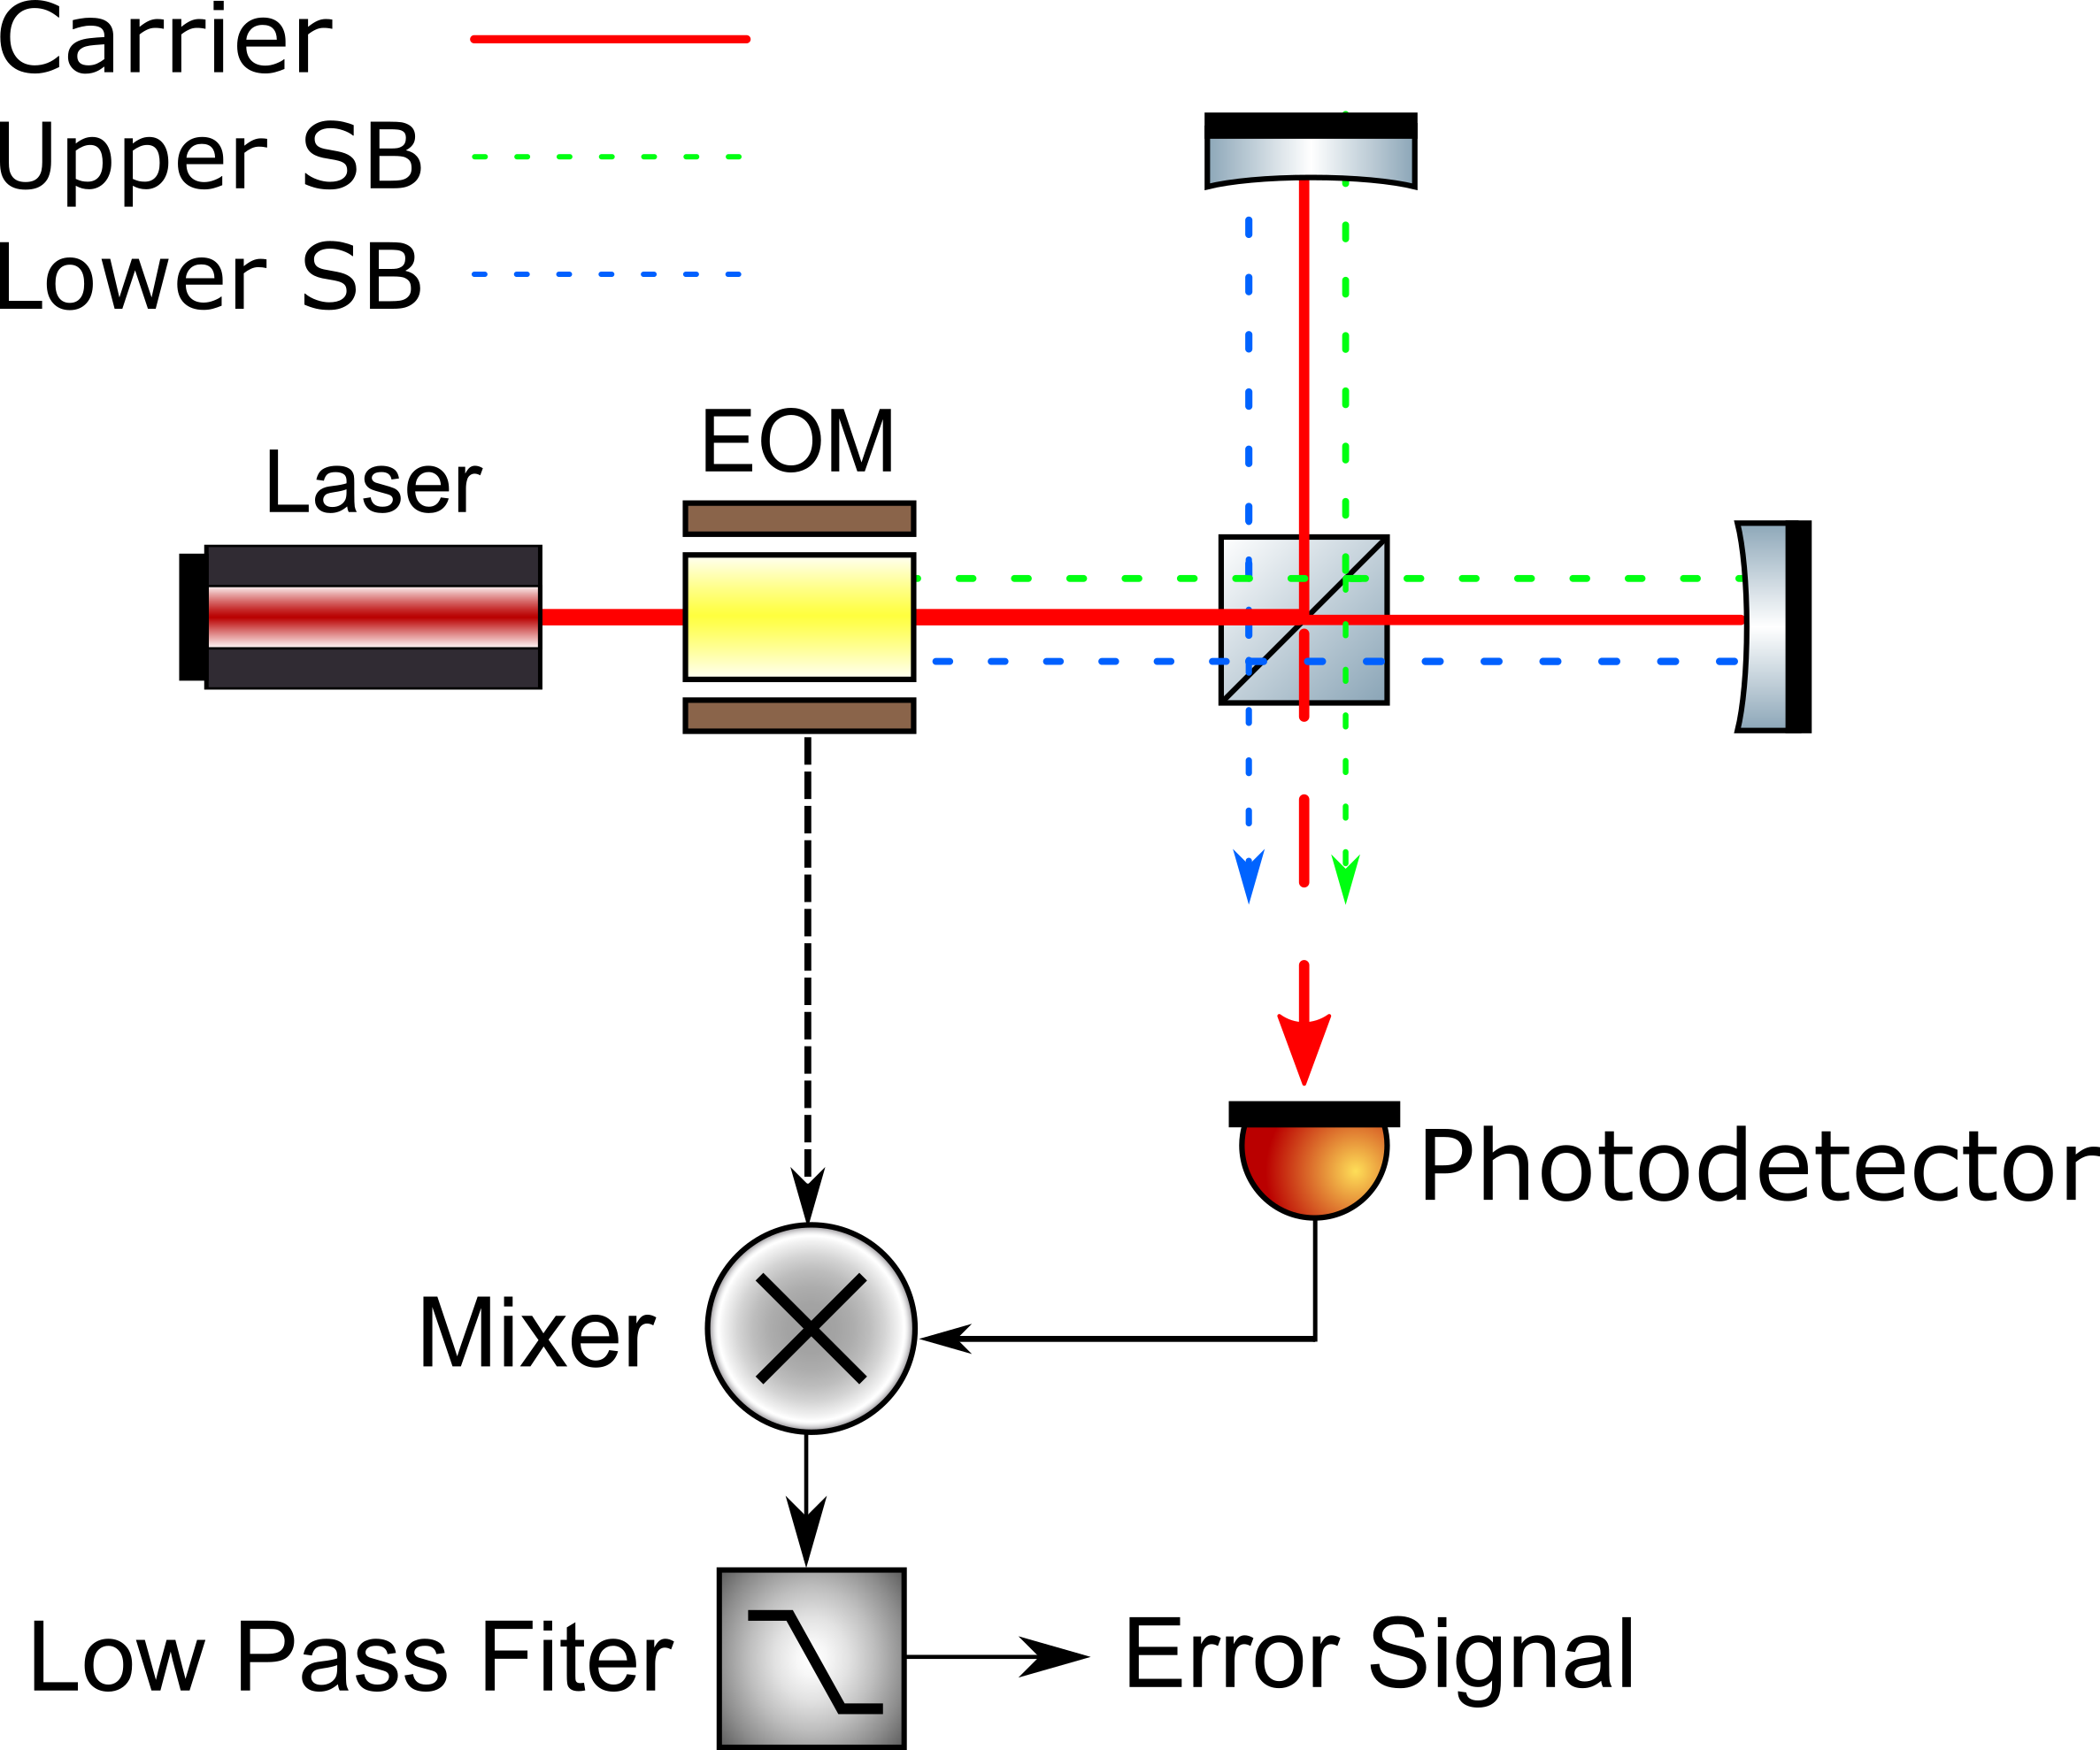
\includegraphics[width=.6 \textwidth]{../Figures/SimpleMichelsonHetero.png}
			\caption[A heterodyne detection scheme for interferometers.]  
			{\textbf{A heterodyne detection scheme for interferometers.} The laser enters an electro-optical modulator which creates three fields described by equation \ref{modE} and read out by a photodetector.  The error signal at the output is then filtered and described by equation \ref{eq:SM_hetero}.}
			\label{fig:MichelsonHetero}
		\end{figure}
		
		The	intensity, which is equal to the electric field squared can be described by
		\begin{equation}\label{RFdet}
		\begin{aligned}
			I	= \vert E_{out} \vert^2  =	&\vert E_{C}\vert^2 + \vert E_{SB+}\vert^2 + \vert E_{SB-}\vert^2 \\
										  	& + 2 \mathbf{Re} \{ \; E_{SB+} E^*_{SB-} e^{2i\Omega t} \; \}\\
										  	& + 2 \mathbf{Re} \{ \; (E_{C} E^*_{SB-} +  E_{SB+} E^*_{C} ) e^{i\Omega t} \; \}
		\end{aligned}
		\end{equation}
		The last term is referred to as the $beat$ $note$ between the carrier signal and the sidebands.  It is possible to extract the term at the modulation frequency using a mixer which is an analog device that outputs the product of two inputs. Usually, the same oscillator that was used to modulate the input beam can be one of the mixer inputs, $\cos(\Omega t)$,  so that the demodulated signal is
		\begin{equation}
		\begin{aligned}
		I_{\text{Demod}} 	&\propto \big[ 4 \pi  J_0(\beta) J_1(\beta) \frac{\ell_+}{\lambda}  \sin(k_{\Omega} \Delta \ell)  \; h_{+}\big] \big[ \cos(\Omega t)  \sin(\Omega t + \phi_{Demod}) \big] \\
					&\propto \big[ 4 \pi  J_0(\beta) J_1(\beta) \frac{\ell_+}{\lambda}  \sin(k_{\Omega} \Delta \ell)  \; h_{+}\big] \big[ \sin(\phi_{Demod}) + \sin(2\Omega t + \phi_{Demod}) \big]
		\end{aligned}
		\end{equation}
		where $\phi_{\text{Demod}}$ is the phase that can be set by the user in order to account for extra phase shifts (ie. longer cables). After the mixer, there will be signals at DC, $\Omega$, $2\Omega$ and so on. However, the part that is linear in the gravitational wave amplitude will be at DC so a low-pass filter will allow the final signal to dominate \cite{BlackPDH}:
		\begin{equation}\label{eq:SM_hetero}
		S = 4 \pi  J_0(\beta) J_1(\beta) \frac{\ell_+}{\lambda}  \sin(k_{\Omega} \Delta \ell) \sin(\phi_{Demod}) \; h_{+}
		\end{equation}
		This shows that a RF detection technique will be linear in GW signal with no large DC offset. Setting the carrier on a null point means $\Delta \ell = \frac{k_{\Omega}}{k} \frac{\pi}{2}$ and allows the designer to optimize the Schnupp asymmetry length to get the best signal for some modulation frequency. This type of readout scheme was used in Enhanced LIGO and is called heterodyne detection, where the sideband fields are produced by an EOM and its efficacy depends on the local oscillator's stability \cite{FritschelReadout}.  
		In contrast, the Advanced LIGO scheme uses a homodyne detection \cite{HildDCReadout} method called "DC-Readout".  Here the oscillator field is produced by slightly offsetting the arms away from the dark fringe and letting a small amount of carrier light through the antisymmetric port.  A gravitational wave will induce sidebands on the carrier and this will allow the same mathematics as above to achieve a linear signal in gravitational wave strain. This method benefits from naturally being co-aligned and mode matched with the signal field.  All techniques follow the same logic of beating the field containing useful information with a reference field to extrapolate a linear signal but the differences come from technical noise such as laser intensity fluctuations and effective quantum noise.
	
		\subsection{Fabry-Perot Cavities}\label{FP}
		There are two ways to improve the LIGO detectors: one is to increase the response from gravitational waves and the other is to decrease the noise contributions. From equation \ref{diffphase}, the gravitational wave signal is proportional to the optical path length that the photon travels, which means the most straightforward method of increasing the sensitivity is to make the arms as long as possible (up to the null point described by equation \ref{gwsinc}).  There are two methods to achieve this: a Herriott delay line or a Fabry-Perot resonator, the differences between each method is shown in Figure \ref{fig:FPvDL}.  At the time of writing this thesis, all modern gravitational wave detectors use the latter method.
		
		\begin{figure}[h]
		\centering
		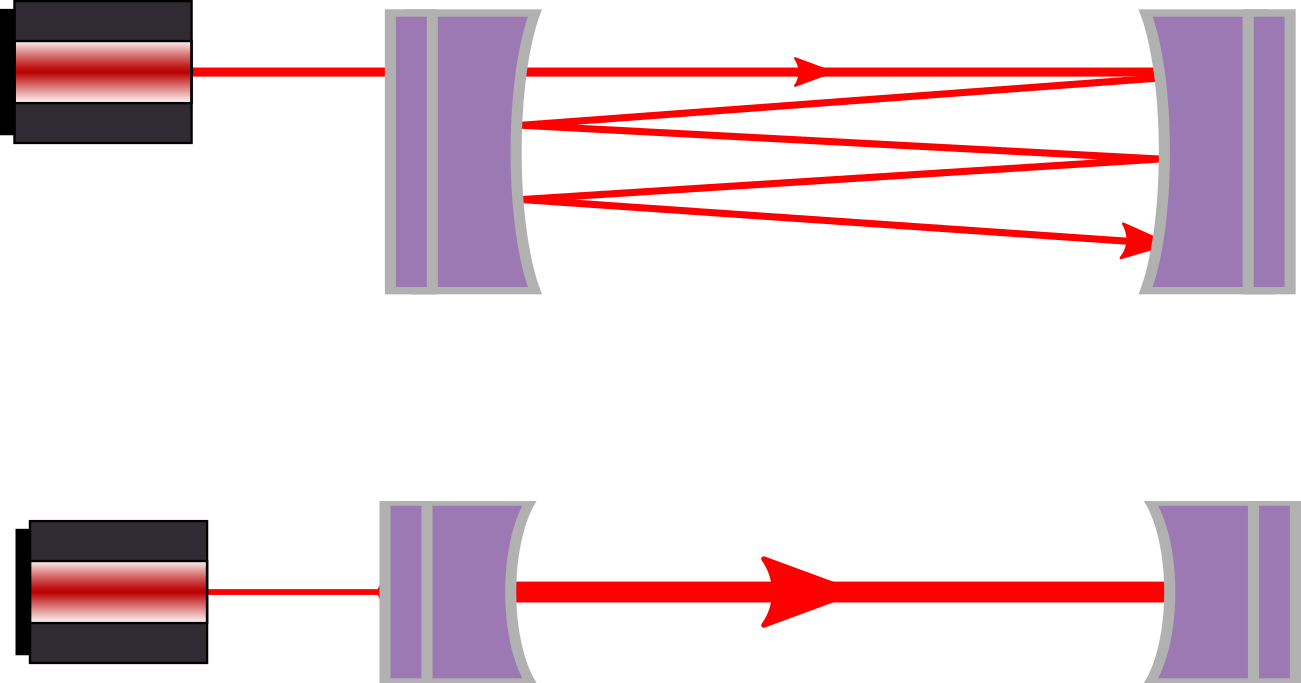
\includegraphics[width=.5 \textwidth]{../Figures/FPvDL.png}
		\caption{Delay Line (top) vs Fabry Perot (bottom)}
		\label{fig:FPvDL}
		\end{figure}
	
		A Fabry-Perot cavity is an optical system comprised of two or more partially transmitting mirrors with one laser input.  To create such a resonator, the user must design a system so that once the electric field has made one round trip within the optical system, the phase of the beam is the same as when it started such that it constructively interferes.  This is done by changing the cavity length, which may seem simple conceptually but in practice, controlling and sensing any optical cavity comes with a few challenges.
		
		To start understanding the longitudinal degree of freedom, consider a two mirror system in Figure \ref{fig:FPvDL} which is separated by a length $L$ with reflection and transmission coefficients: $r_1$, $t_1$, $r_2$, $t_2$.  Starting with a plane wave at the input mirror with amplitude $E_0$, the beam will enter the cavity and propagate back between the two mirrors.  The reflected, transmitted, and circulating fields \cite{Saulson}, which are a result of the geometric series, can be described as
		\begin{equation}\label{r_FP}
		E_{\text{REFL}} = r_{FP} E_0 = \bigg(-r_1 + \frac{t_1^2 r_2  e^{-i2kL}}{1-r_1 r_2 e^{-i2kL}} \bigg) E_0
		\end{equation}
		\begin{equation}\label{t_FP}
		E_{\text{TRAN}} = t_{FP} E_{0} = \bigg( \frac{t_1 t_2 e^{ikL}}{1-r_1 r_2 e^{-i2kL}}\bigg) E_0
		\end{equation}
		\begin{equation}\label{c_FP}
		E_{\text{CIRC}} = c_{FP} E_0 = \bigg(\frac{t_1}{1- r_1 r_2 e^{-2ikL}} \bigg) E_0
		\end{equation}
		The above fields are all highly dependent on the round trip phase accumulated within the cavity which becomes resonant when the length is $L = n \lambda / 2$. While on resonance, the circulating coefficient in the cavity is maximized such that the gain is
		\begin{equation}
		\text{Gain} = c^2_{FP} \vert_{\text{resonating}} = \bigg( \frac{t_1}{1-r_1 r_2}\bigg)^2
		\end{equation}
				\begin{figure}[ht]
			\centering
			\begin{subfigure}[b]{0.45\textwidth}
				\centering
				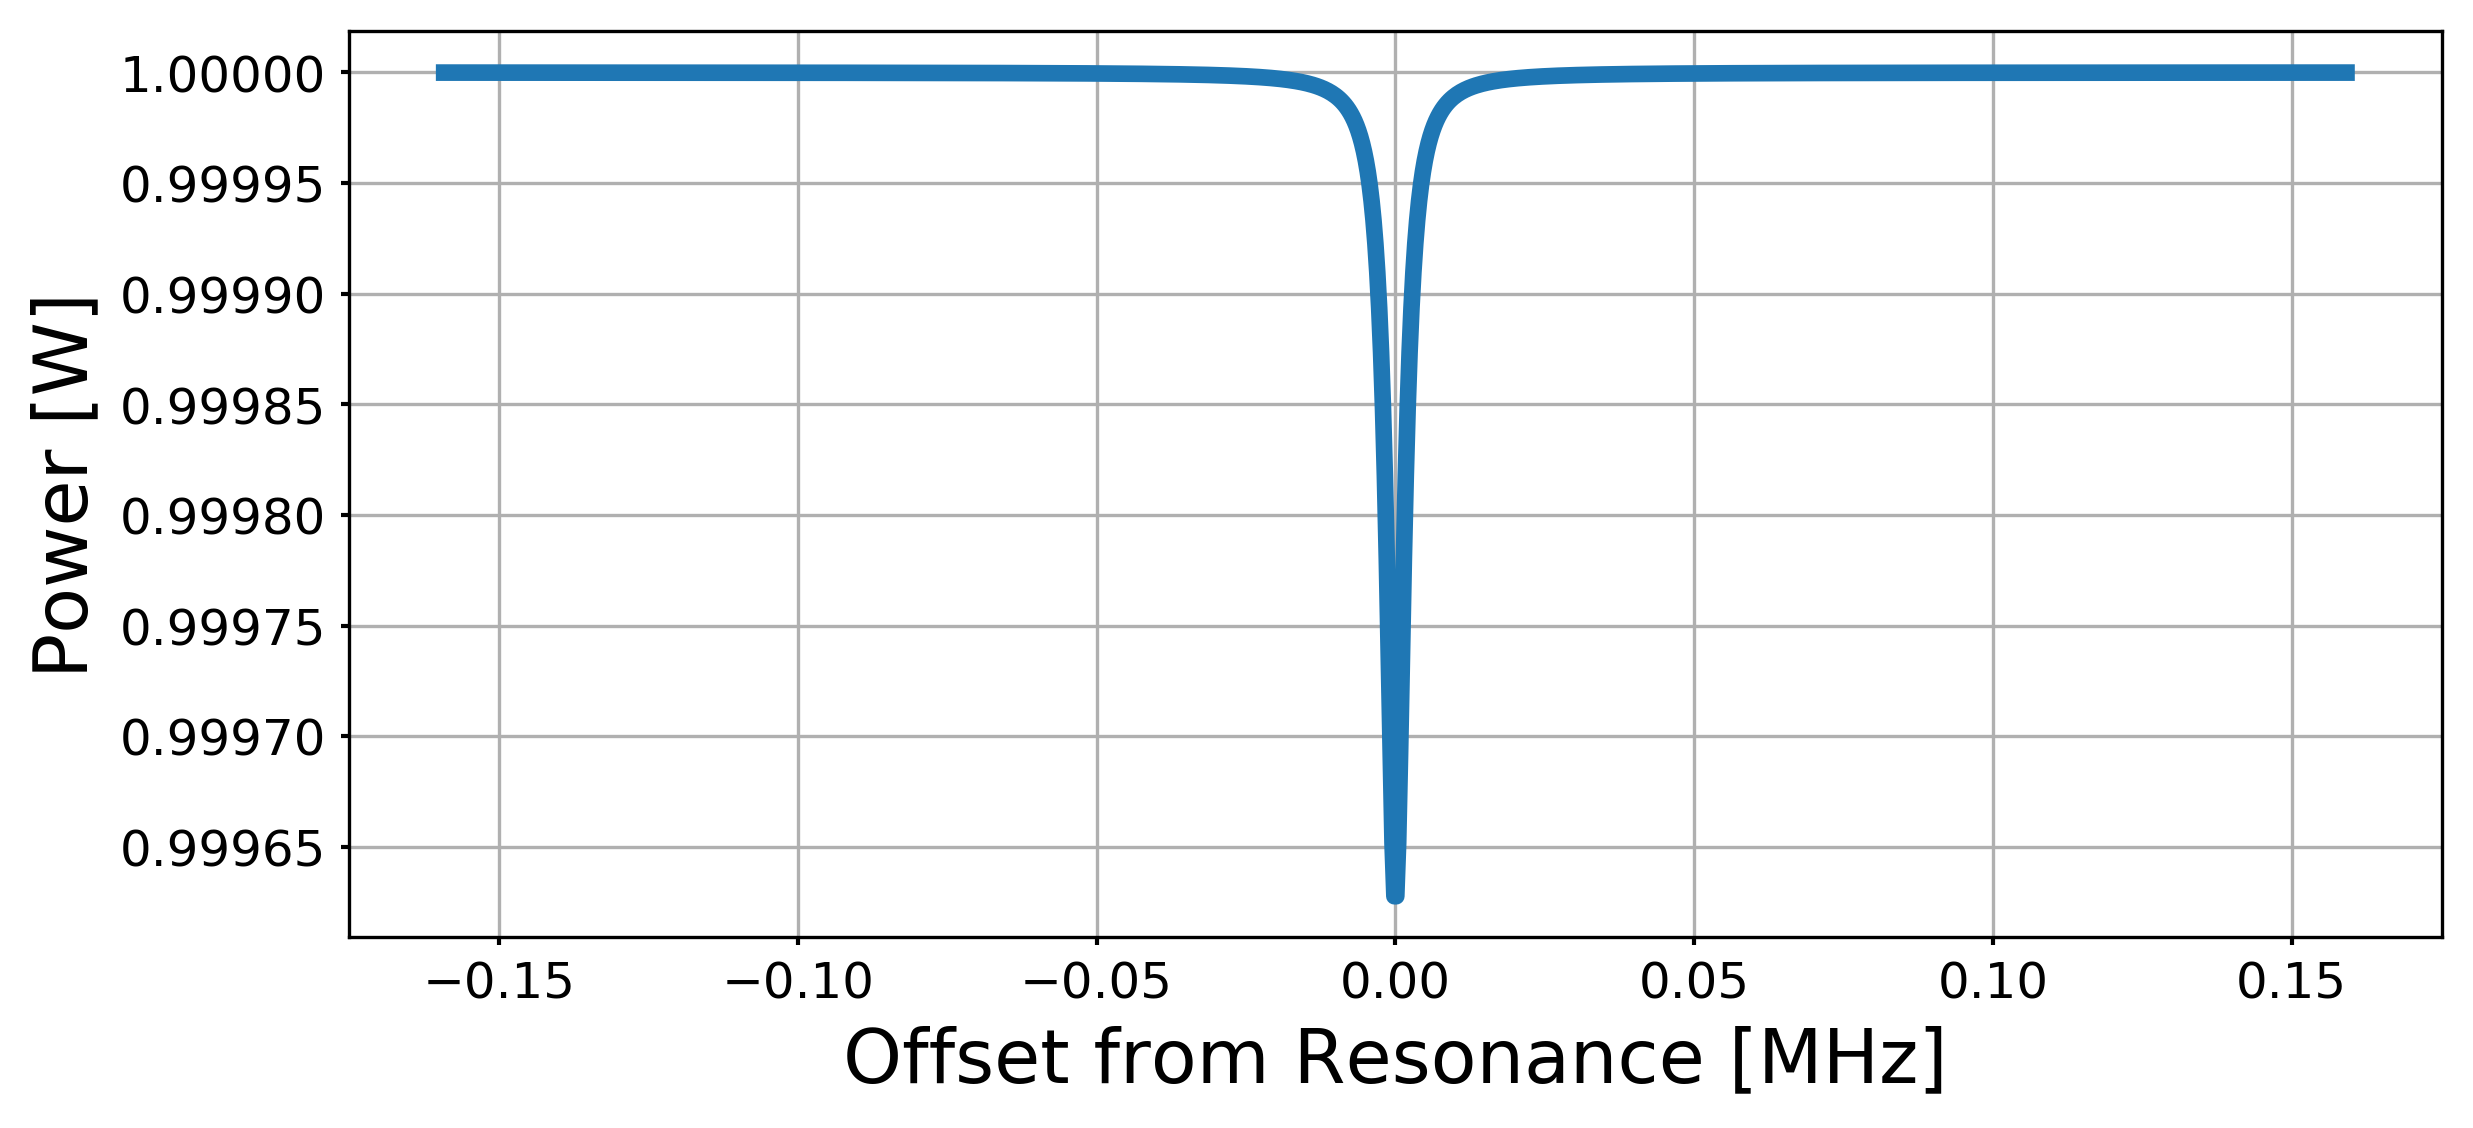
\includegraphics[width=\textwidth]{../Figures/Arm_Refl.png}
				\caption{Reflected Power}
				\label{fig:FP_refl}
			\end{subfigure}
			\hfill
			\begin{subfigure}[b]{0.45\textwidth}
				\centering
				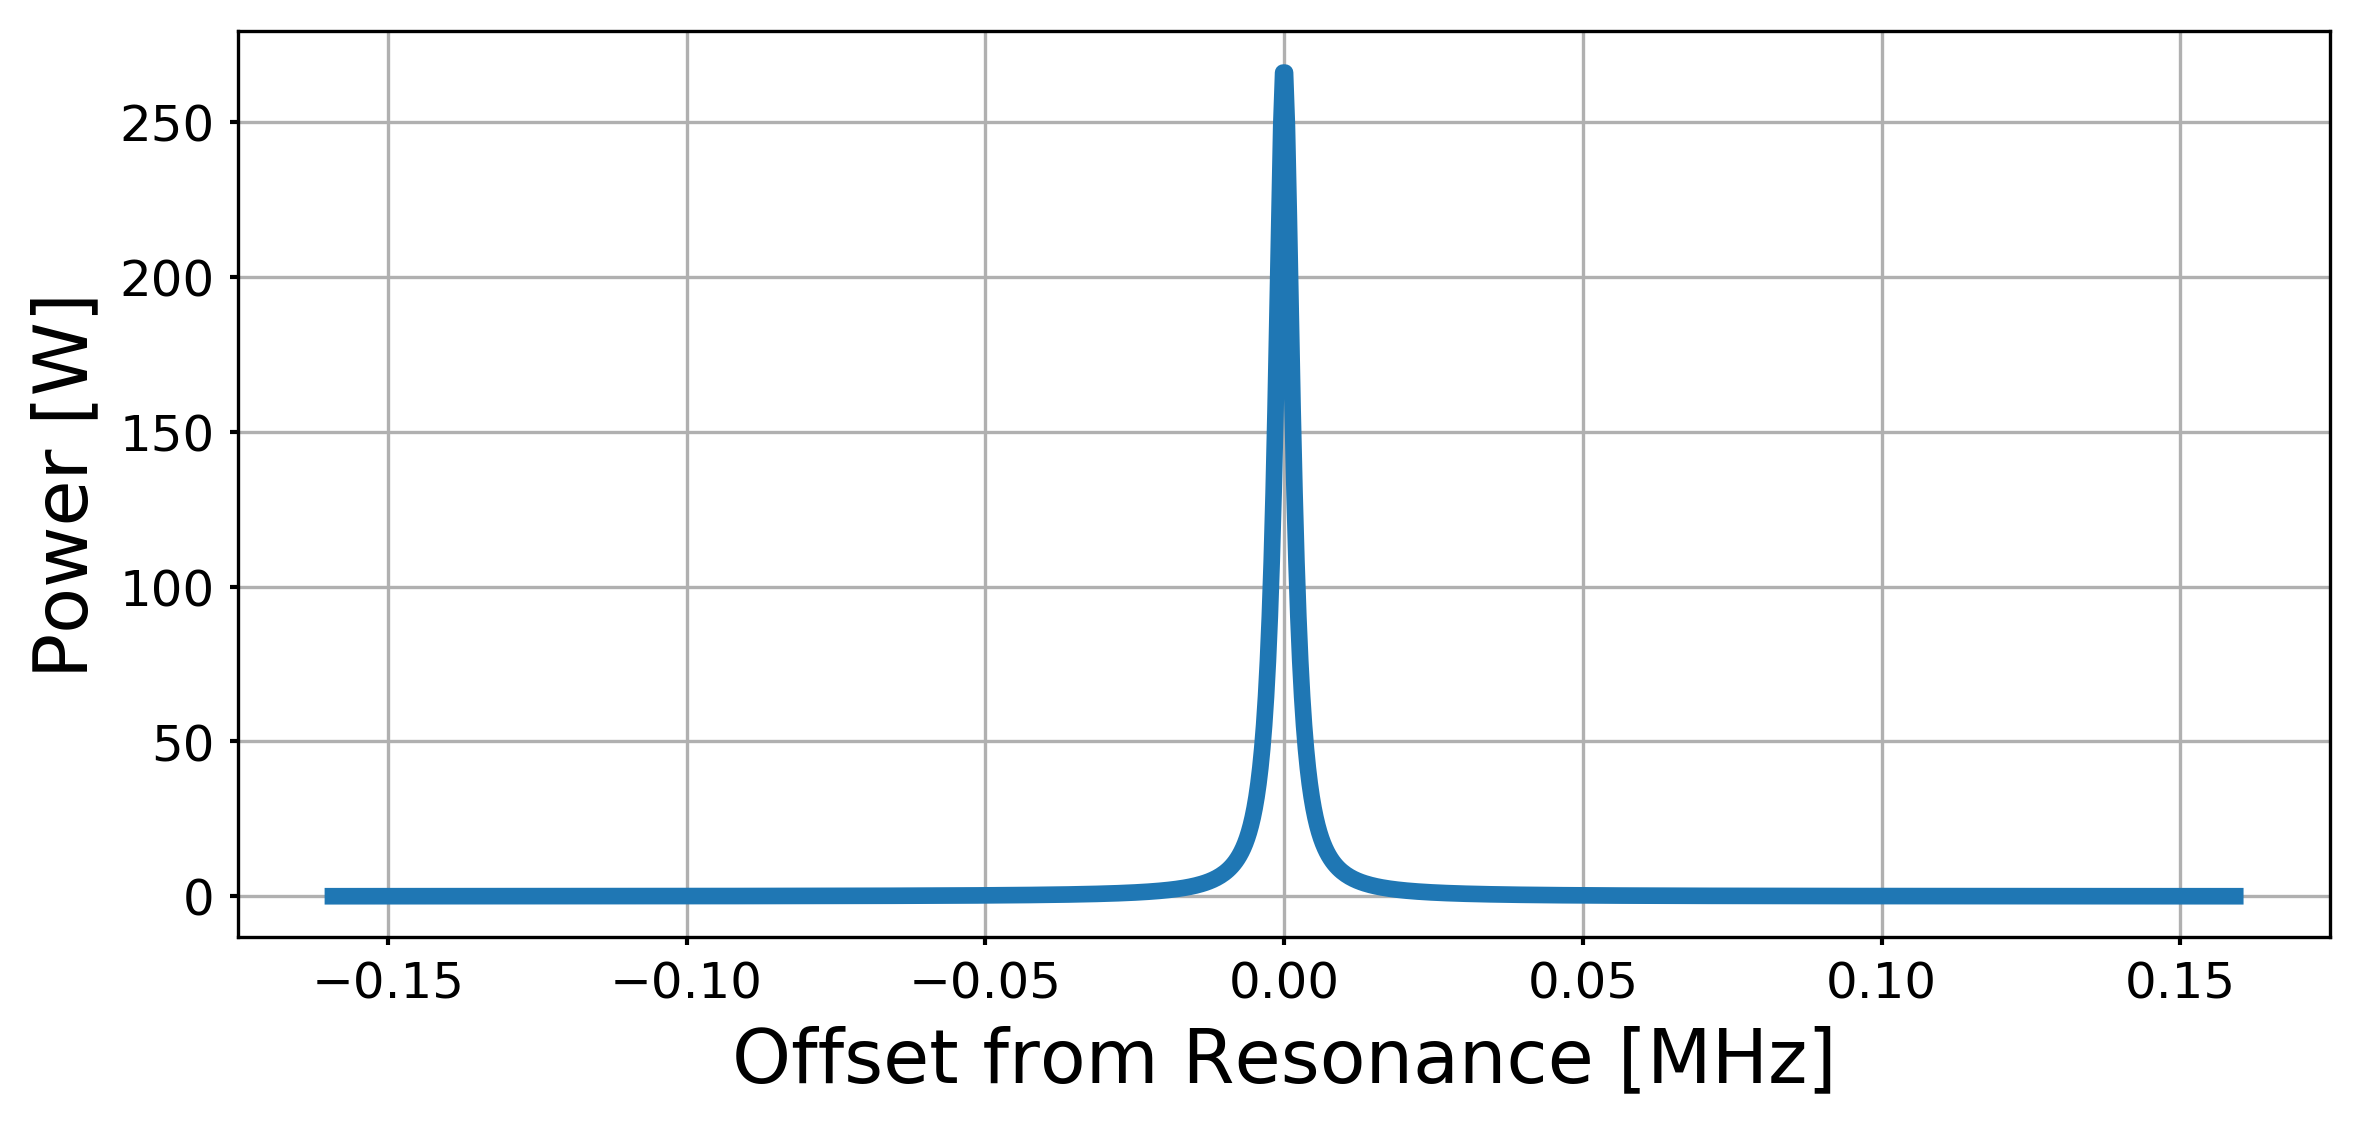
\includegraphics[width=\textwidth]{../Figures/Arm_Circ.png}
				\caption{Circulating Power}
				\label{fig:FP_circ}
			\end{subfigure}
			\hfill
			\begin{subfigure}[b]{0.45\textwidth}
				\centering
				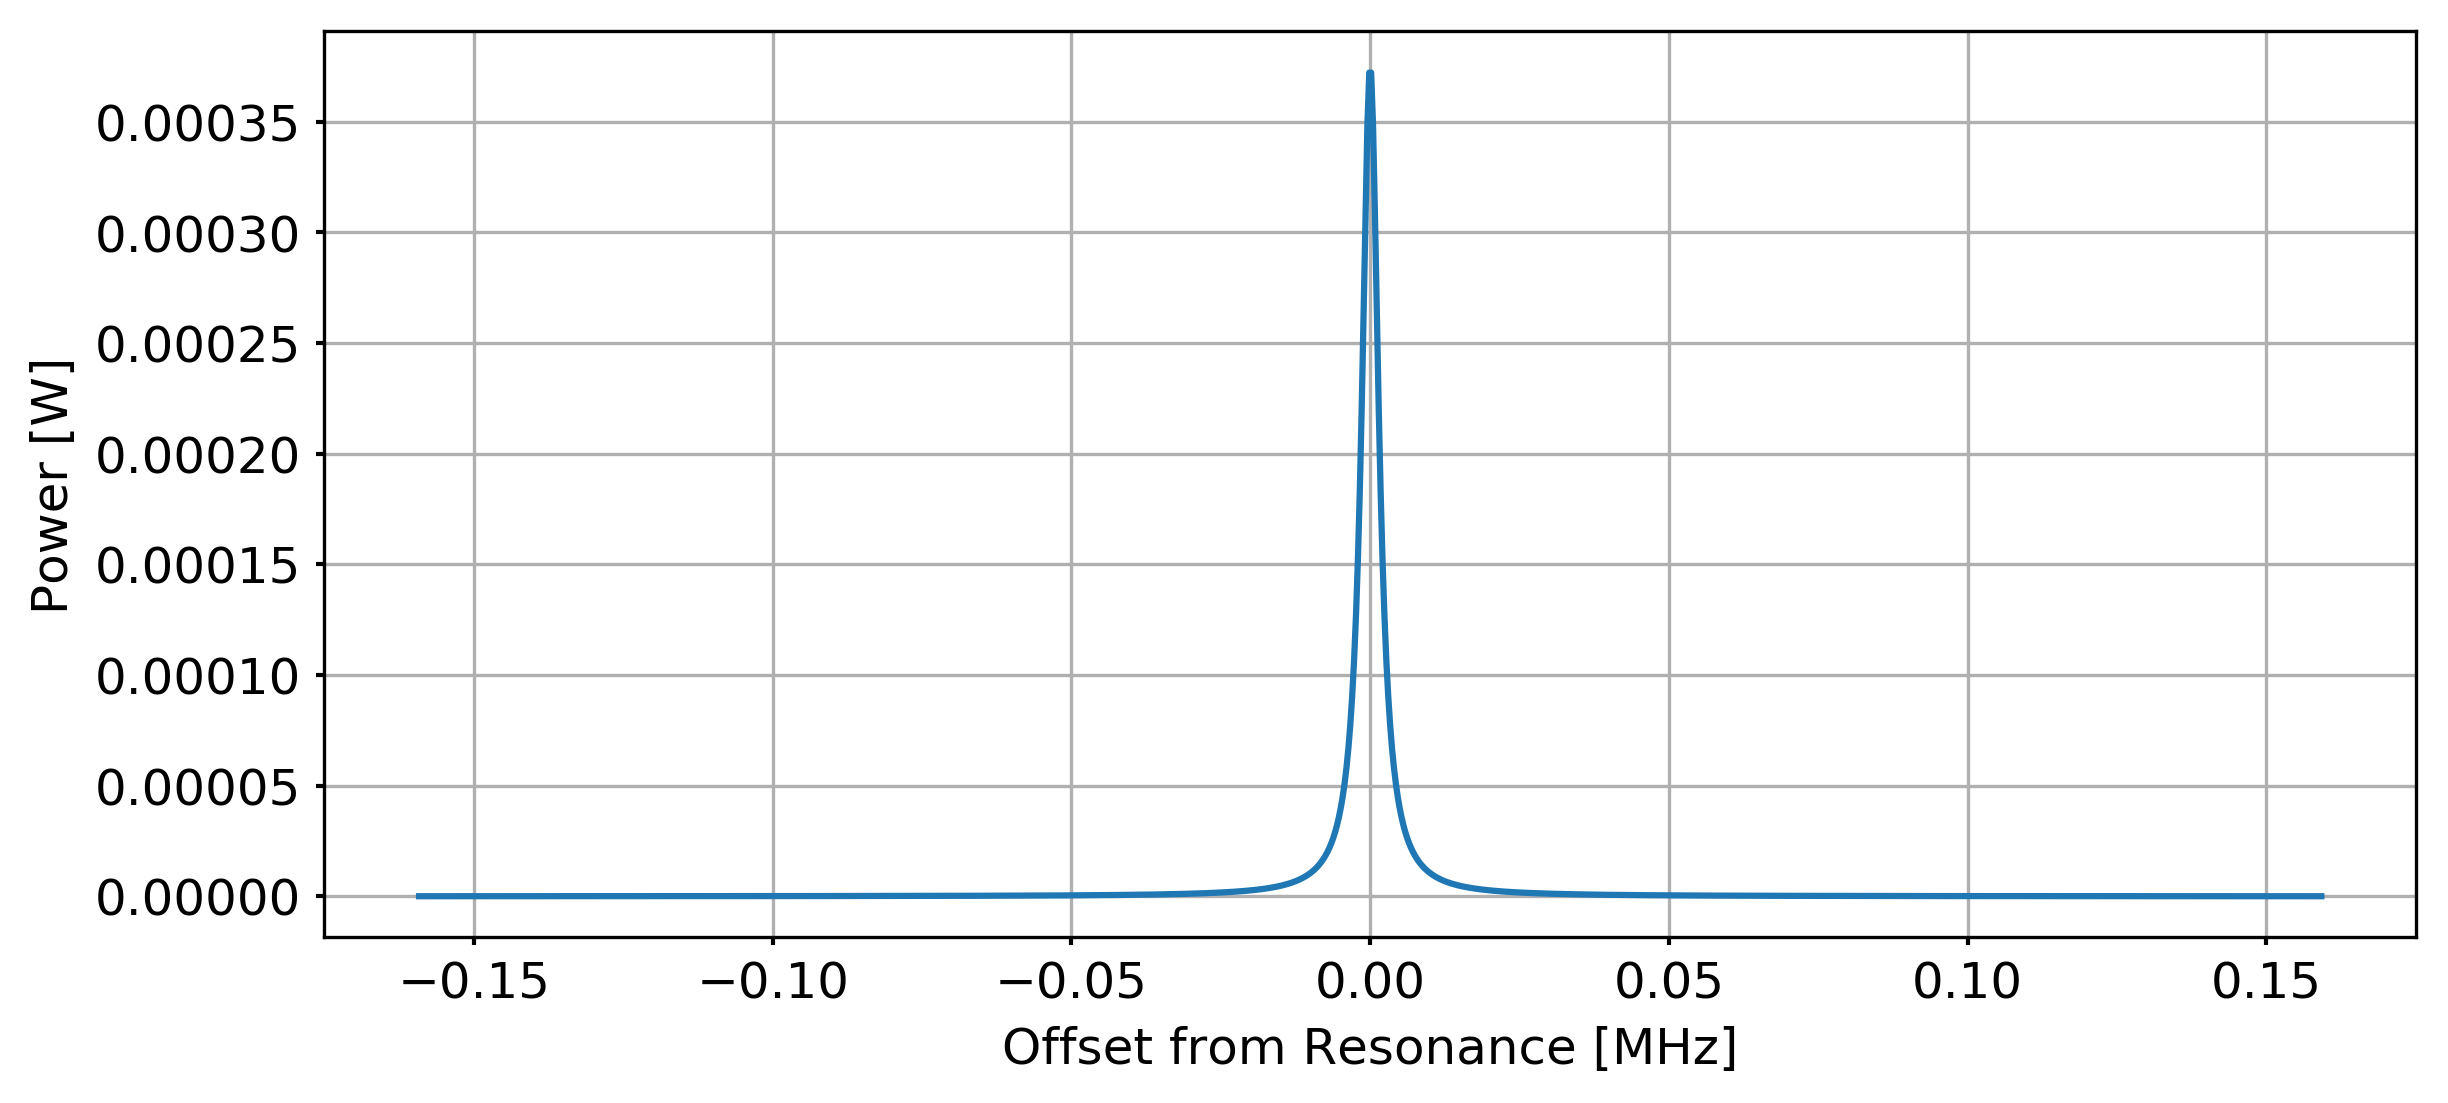
\includegraphics[width=\textwidth]{../Figures/Arm_Tran.png}
				\caption{Transmitted Power}
				\label{fig:FP_tran}
			\end{subfigure}
			\caption[The reflected, circulating, and transmitted powers for a single Fabry-Perot cavity.]
			{The  has properties in Table [] to represent one of the LIGO 4km arms which are highly over-coupled cavities so almost all of the light reflects toward the beamsplitter.  The input power is normalized to 1 Watt to show the relative gain of the circulating power.}
			\label{fig:FP_pwrs}
		\end{figure}
		Notice that the fields are dependent on the cavity length and laser frequency, $2kL$, so one might naively determine that modulating the two parameters independently cause the same effect.  However, when both are changing by large amounts, they are related by a frequency dependent transfer function \cite{dynamicFP}
		\begin{equation}
		C(\omega) \frac{\Delta \omega}{\omega} = -\frac{\Delta L}{L}
		\end{equation}
		where $C(\omega) = \frac{1-e^{-2i\omega L/c}}{2i\omega L/c}$. It is only when the cavity is on resonance that the frequency and length variations are related by $\frac{\Delta w}{w} = -\frac{\Delta L}{L}$.
		Depending on the relative reflection coefficients of the input and output mirrors, the fields on resonance will be different in amplitude.  For example, in the LIGO 4 km arms, the end test masses are highly reflective with a transmission of about 4 parts per million while the input test masses have a transmission of about 0.015.  This means that the arm cavities are very much over-coupled and almost all of the light reflects back towards the beamsplitter.
		\begin{figure}[ht]
			\centering
			\begin{subfigure}[b]{0.45\textwidth}
				\centering
				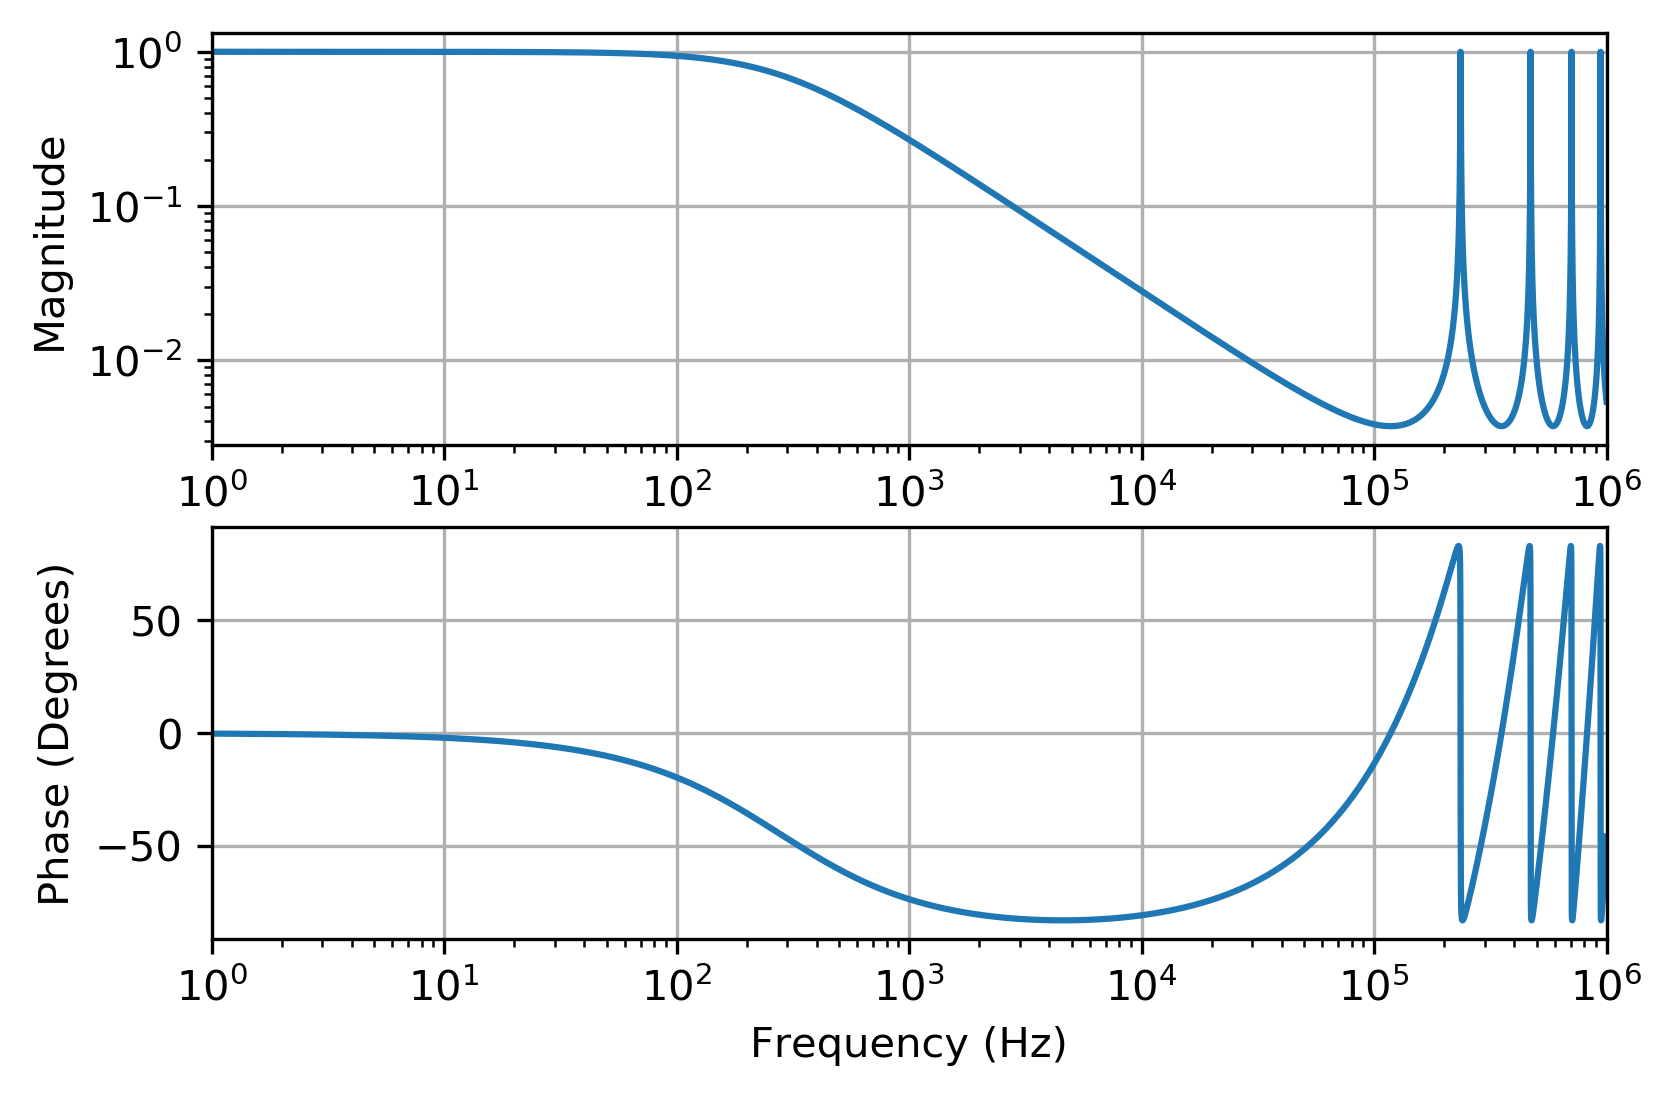
\includegraphics[width=\textwidth]{../Figures/FP_L_TF.png}
				\caption{Transfer function with respect to L}
				\label{fig:FP_L}
			\end{subfigure}
			\hfill
			\begin{subfigure}[b]{0.45\textwidth}
				\centering
				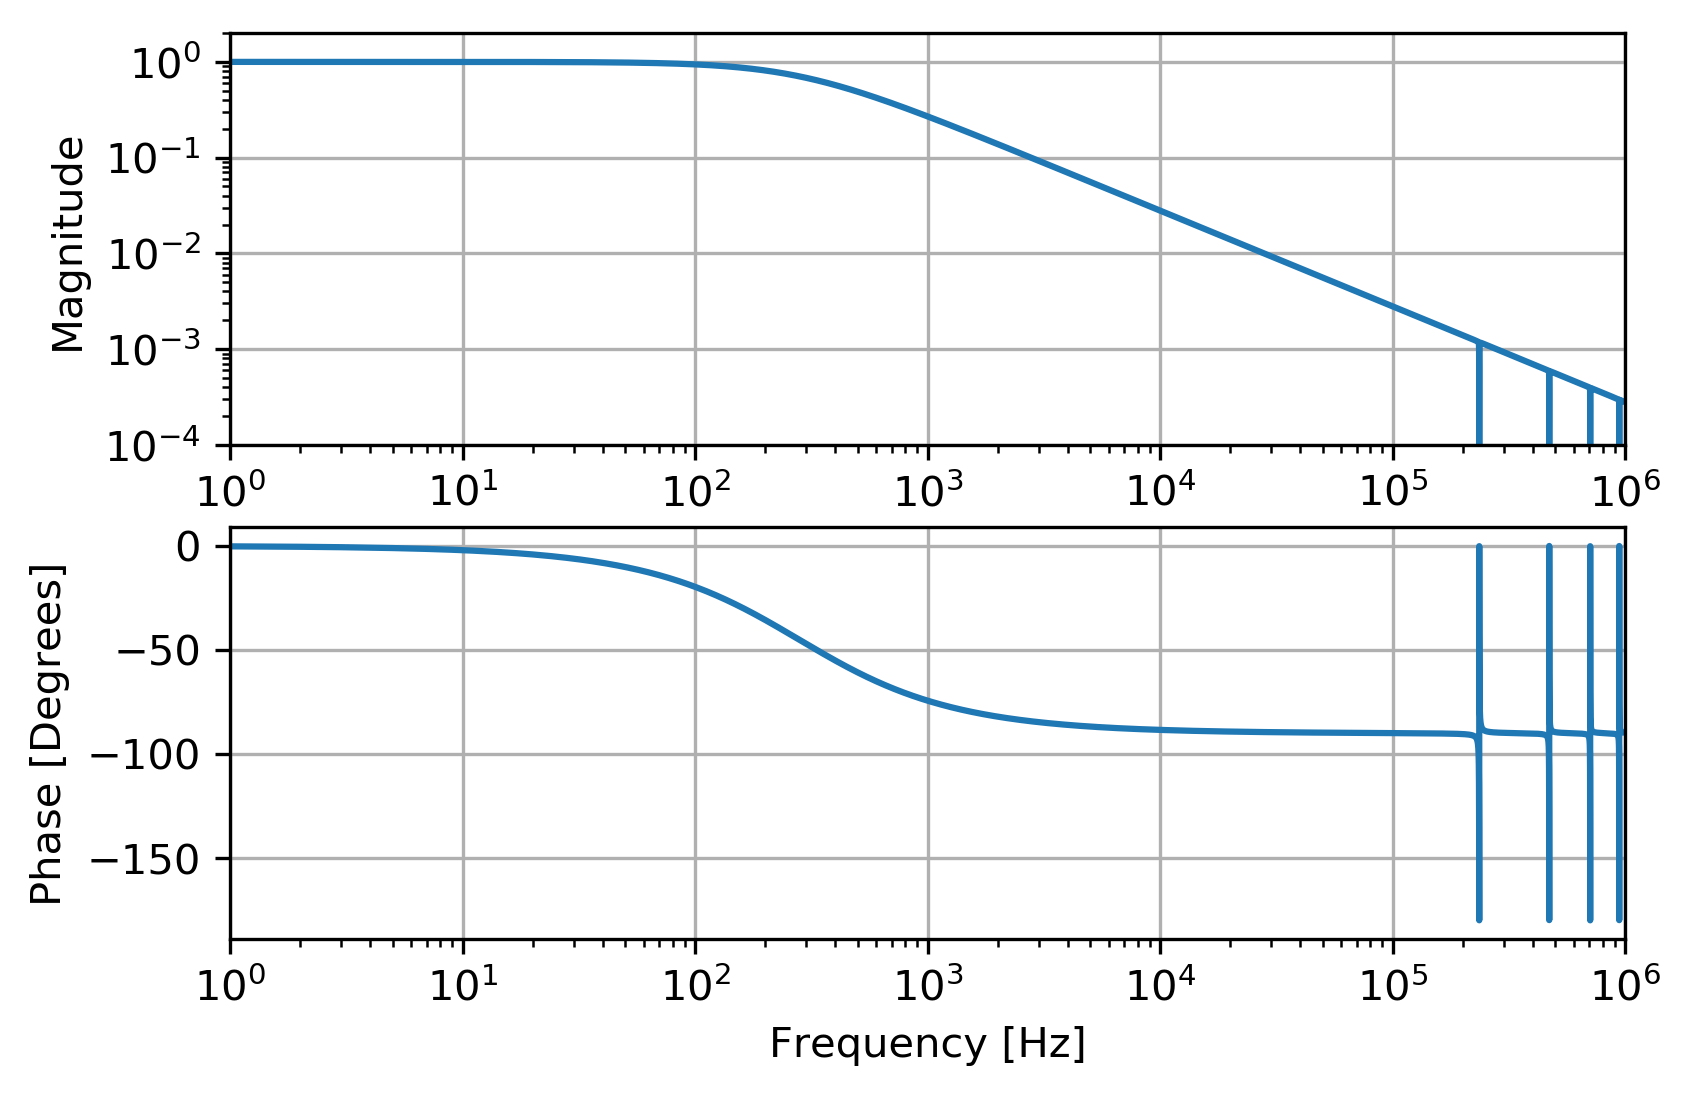
\includegraphics[width=\textwidth]{../Figures/FP_F_TF.png}
				\caption{Transfer function with respect to F}
				\label{fig:FP_F}
			\end{subfigure}
			\caption{Bode Plots of a linear Fabry-Perot response in reflection.}
			\label{fig:FP_Bode}
		\end{figure}
		It is important to understand the Fabry-Perot response while sweeping through either the laser frequency or cavity length and measuring the reflected (or transmitted) fields, there are features of the power spectrum which relate directly to the cavity's physical properties.
		
		The finesse describes the line width of the resonant peak and is function of $r_1$ and $r_2$.  A higher finesse will mean the line width is smaller and taller:
		\begin{equation}\label{finesse}
		\mathbb{F} = \frac{\pi \sqrt{r_1 r_2}}{1- r_1 r_2}
		\end{equation}
		The cavity storage time, $\tau_s$, describes how long it takes the power circulating in the cavity to decay by a factor of $1/e$ if the laser suddenly turns off,
		\begin{equation}
		\tau_{s} = \frac{L}{c \pi} \, \mathbb{F}
		\end{equation}
		The pole frequency, $f_{\text{pole}}$, is when the magnitude of the cavity's transfer function (see Figure \ref{fig:FP_Bode} ) reaches 3db below the DC level:
		\begin{equation}
		f_{\text{pole}} = \frac{1}{4\pi \tau_{s}}
		\end{equation}
		The free spectral range,$f_{\text{FSR}}$, is the frequency span from one resonant peak to the next.
		\begin{equation}
		f_{\text{FSR}}  = \frac{c}{2L}
		\end{equation}
		It is useful to understand the power circulating as a function of our defined parameters slightly off resonance by a length of $\Delta L$
		\begin{equation}
		P_{cav} = \vert c_{FP} \vert^2 = \frac{\text{Gain}}{ 1 + \big(\frac{2\mathbb{F}}{\pi} \big)^2 \, \text{sin}^2(k \Delta L) }
		\end{equation}
		In order to prove that an optical cavity is stable, it is useful to introduce the matrices that describe a periodic optical system which is explicitly derived in appendix \ref{FPappendix}.  A Fabry Perot cavity that is separated by distance $L$ with spherical mirrors that have radii of curvature $R_1$ and $R_2$ will need to satisfy 
		\begin{equation}\label{gfactor}
		0 \leq \bigg(1-\frac{L}{R_1}\bigg) \bigg(1-\frac{L}{R_2}\bigg) \leq 1
		\end{equation}
		in order to be geometrically stable.
		
		LIGO uses the frequency response of optical cavities for a number of reasons: Firstly, the round trip phase of the gravitational wave is amplified by the finesse (equation \ref{finesse}) of the 4 kilometer arm cavities, therefore increasing the sensitivity.  Secondly, the input and output of the interferometer's Gaussian beam mode can be refined by only allowing the fundamental mode of the laser to resonate (input and output mode cleaners).  Thirdly, Advanced LIGO uses a dual-recycled Michelson interferometer which means the symmetric port has a mirror inserted to resonate the light reflected from the Fabry Perot arms (power recycling) and another mirror shapes the frequency response of the differential cavity pole at the anti-symmetric port (signal recycling).
		
		\subsubsection{Achieving Resonance in an Optical Cavity}
		Described above are the theoretical constructs for a Fabry-Perot cavity, but the question remains, how does one practically construct a resonant optical cavity?  The answer comes from using a heterodyne sensing scheme similar to the one described in Section \ref{michelson}.  Except the optical system is not a Michelson interferometer but rather a two mirror cavity and can apply to a number of different geometries such as triangular or bow-tie cavities.
		
		Starting with an input laser and EOM (electro-optical modulator) that imparts upper and lower sidebands at a modulation frequency $\Omega$, the user injects three beams into the optical system described in Equation \ref{modE}.  When placing a photodetector on the reflection port, one should see the cavity's effect on each of the three electric fields.
		
		\begin{equation}
		E_{FP,out} = E_{C} + E_{SB+} + E_{SB-} = 
		\begin{pmatrix}
		r_{C} 	&   
		\\ 	r_{SB+} &
		\\ 	r_{SB-} &
		\end{pmatrix}
		\begin{pmatrix}
		E_{C,in} &    E_{SB+,in}    &  E_{SB-,in}     
		\end{pmatrix}
		\end{equation}
		
		where the reflection coefficients follow equation \ref{r_FP}.  Because sidebands are frequency shifted, they will effectively $see$ a different cavity than the carrier and the total phase accumulated by the two fields will be different. To make a good reference for the resonant carrier beam, the modulation frequency $k_{\Omega}$, is chosen such that sidebands are be anti-resonant which effectively means they are rejected from entering the cavity.
		\begin{equation}
		r_{C} = -r_1 + \frac{t_1^2 r_2  e^{-i2kL}}{1-r_1 r_2 e^{-i2kL}}
		\end{equation}
		and 
		\begin{equation}
		r_{SB\pm} = -r_1 + \frac{t_1^2 r_2  e^{-i2(k+k_{\Omega})L}}{1-r_1 r_2 e^{-i2(k+k_{\Omega})L}}
		\end{equation}
		The formalism to read out the error signal is the shown in Equation \ref{RFdet} where a photodetector in reflection (see Figure \ref{fig:FPControl}) reads out the sum of fields squared and demodulates to get the error signal which will be linearly proportional to the laser frequency and cavity length \cite{BlackPDH}.
		\begin{equation}
		\text{Error Signal} \propto \frac{L \mathbb{F}}{\lambda} \bigg[\frac{\delta w}{w} + \frac{\delta L}{L}\bigg]
		\end{equation}
		
		\begin{figure}[h]
		\centering
		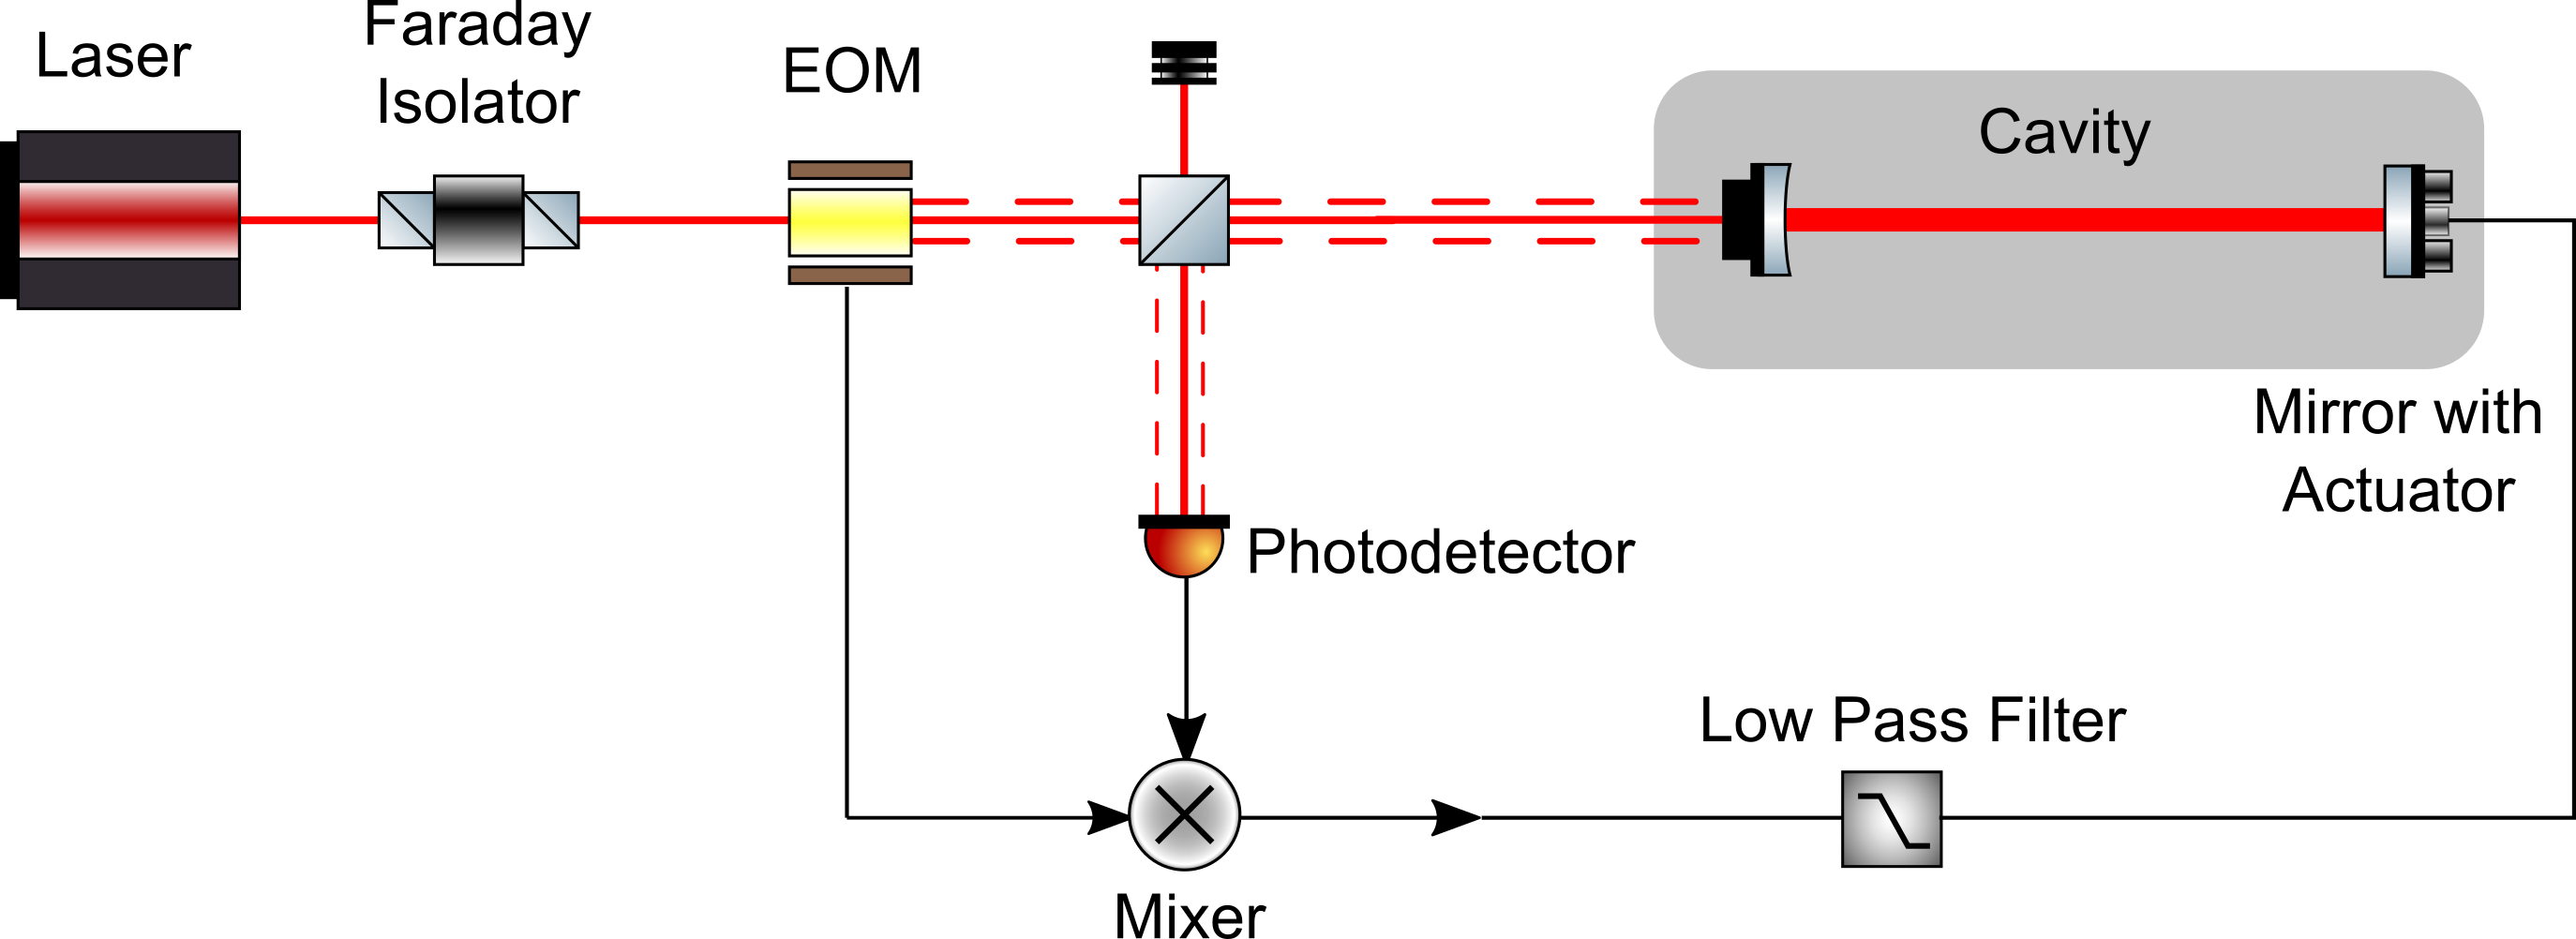
\includegraphics[width=.75 \textwidth]{../Figures/FP_Control.png}
		\caption[Control scheme for an optical cavity.]{\textbf{Control scheme for an optical cavity.} The electric fields in reflection provide the error signal when mixed with the local oscillator and then gets low-passed for a DC signal to drive the end mirror which will control the length of the cavity, see Figure \ref{fig:FP_err}.}
		\label{fig:FPControl}
		\end{figure}
	
		\begin{figure}[h]
		\centering
		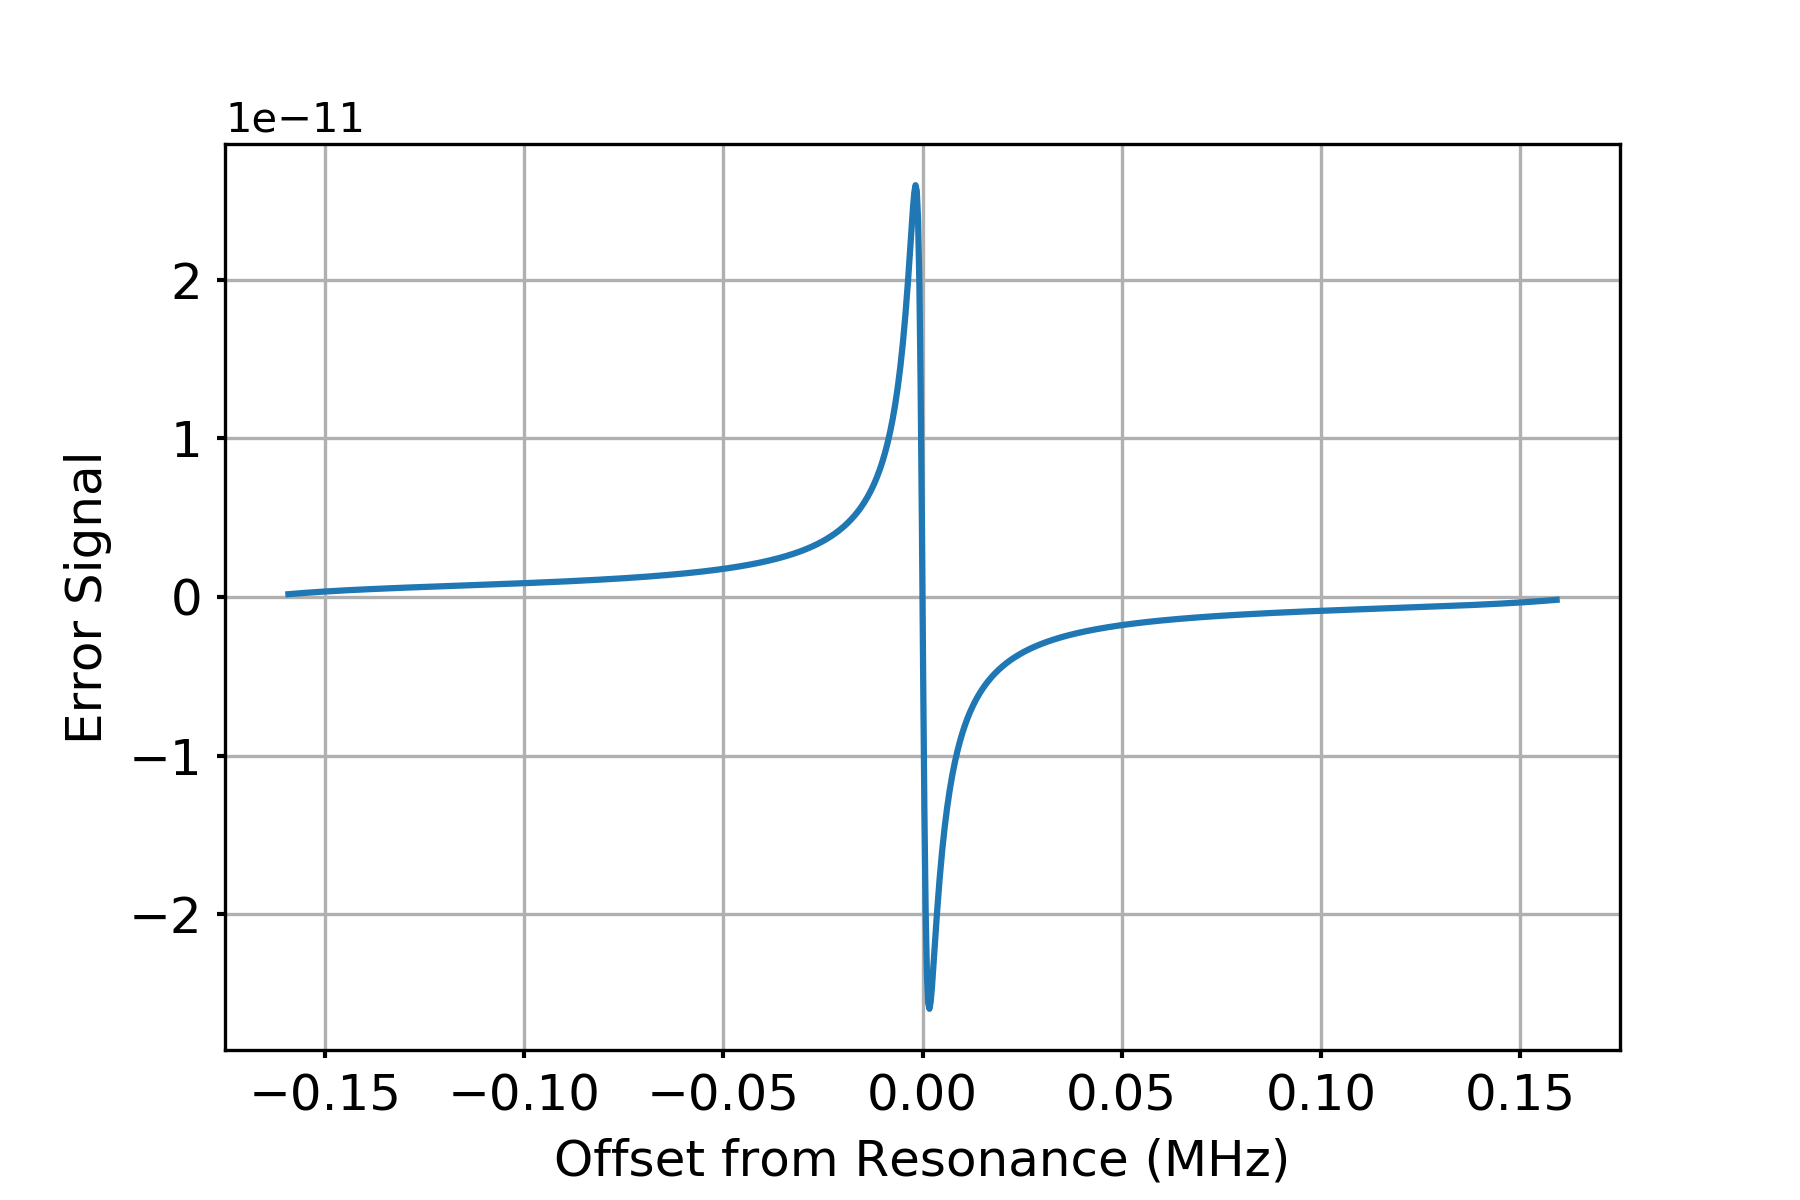
\includegraphics[width=.75 \textwidth]{../Figures/PDH_Err.png}
		\caption[Error signal in reflection]{\textbf{Pound-Drever-Hall (PDH) error signal in reflection of a Fabry Perot cavity.}  By modulating the frequency (or length) close to the zero offset point, the error signal is linear.  However, if the actuation is too far away from the lock point, the signal becomes highly non-linear.  Which means the drive output must wait until the error signal comes close enough to zero before triggering on. }
		\label{fig:FP_err}
		\end{figure}
	
		
		\subsection{Fabry-Perot Michelson}\label{FPmich}
		Using an optical cavity to increase the number of bounces along the 4 kilometer arms will amplify the gravitational wave signal but it will also shape the frequency dependence of the sensitivity as well.  This has already been alluded to in section \ref{measuringGWs} where the overall increase in arm length will tune the response function of equation \ref{gwsinc}.  The same idea can apply to integrate the use of Fabry-Perot arms into a Michelson interferometer and looking at the signal at the antisymmetric port as a function of gravitational wave frequency. Previously in section \ref{sec:michelson}, it was shown that the heterodyne RF detection technique required beating the sidebands with a carrier field containing the gravitational wave information.  However, this is not the only way because the signal sidebands beating with a reference carrier field could also be a valid way of measuring a signal of interest. In fact, Advanced LIGO employs a specific type of homodyne detection called DC readout \cite{FritschelReadout}\cite{FritschelAdvancedLIGO}. The idea is that the carrier field will resonant in the arms but will be slightly modulated due to a gravitational wave which will create audio frequency sidebands imparted on the field.  
		
		Figure \ref{fig:FPMichelson} shows an input electric field of $E_0$ incident on a 50/50 beamsplitter which then enters two orthogonal arm cavities of length $L_x$ and $L_y$.  Notice that the distance from the beamsplitter to the input couplers for both arms denoted by $l_x$ and $l_y$ are independent variables, this is to account for the DARM offset which is analogous to the Schnupp asymmetry described in section \ref{sec:michelson}.  After partially transmitting and reflecting at the beamsplitter, the fields will resonate in each of the arm cavities and obey the reflectivity relations described by equation \ref{r_FP}.  Upon recombining at the beamsplitter, the antisymmetric port electric field will be related to the arm fields by,
		\begin{equation}
		E_{\text{AS}} = \frac{1}{\sqrt{2}} [E_{x}^{\text{ARM}} + E_{y}^{\text{ARM}} ] 
		\end{equation}
		where $E_{i}^{\text{ARM}} = E(\omega) \pm [E(+ \omega_{\text{\tiny GW}}) + E(- \omega_{\text{\tiny GW}})] \sin{k\delta l } $ is the reflected fields for the x and y arms which contain the carrier(first term) and GW signal sidebands(last two terms).  In this case, the gravitational wave sidebands are a single frequency for simplicity but this analysis will work for all frequencies spanning the LIGO sensitivity band.  Intuitively, one can deduce that the antisymmetric port will only be sensitive to the differential motion between the arm cavities, which means the gravitational wave sidebands in the x-arm will be out of phase with the y-arm.  Also it is important to note that inserting a DC microscopic length shift of a few picometers represented by $\delta l = l_x - l_y$ allows for some carrier leakage field to propagate towards the antisymmetric port which creates the static reference to form a beat note with the signal sidebands.  The same effect can be achieved by introducing a static offset between the x and y arms; colloquially, this is referred to as DARM offset.
				
		\begin{figure}[ht]
			\centering
			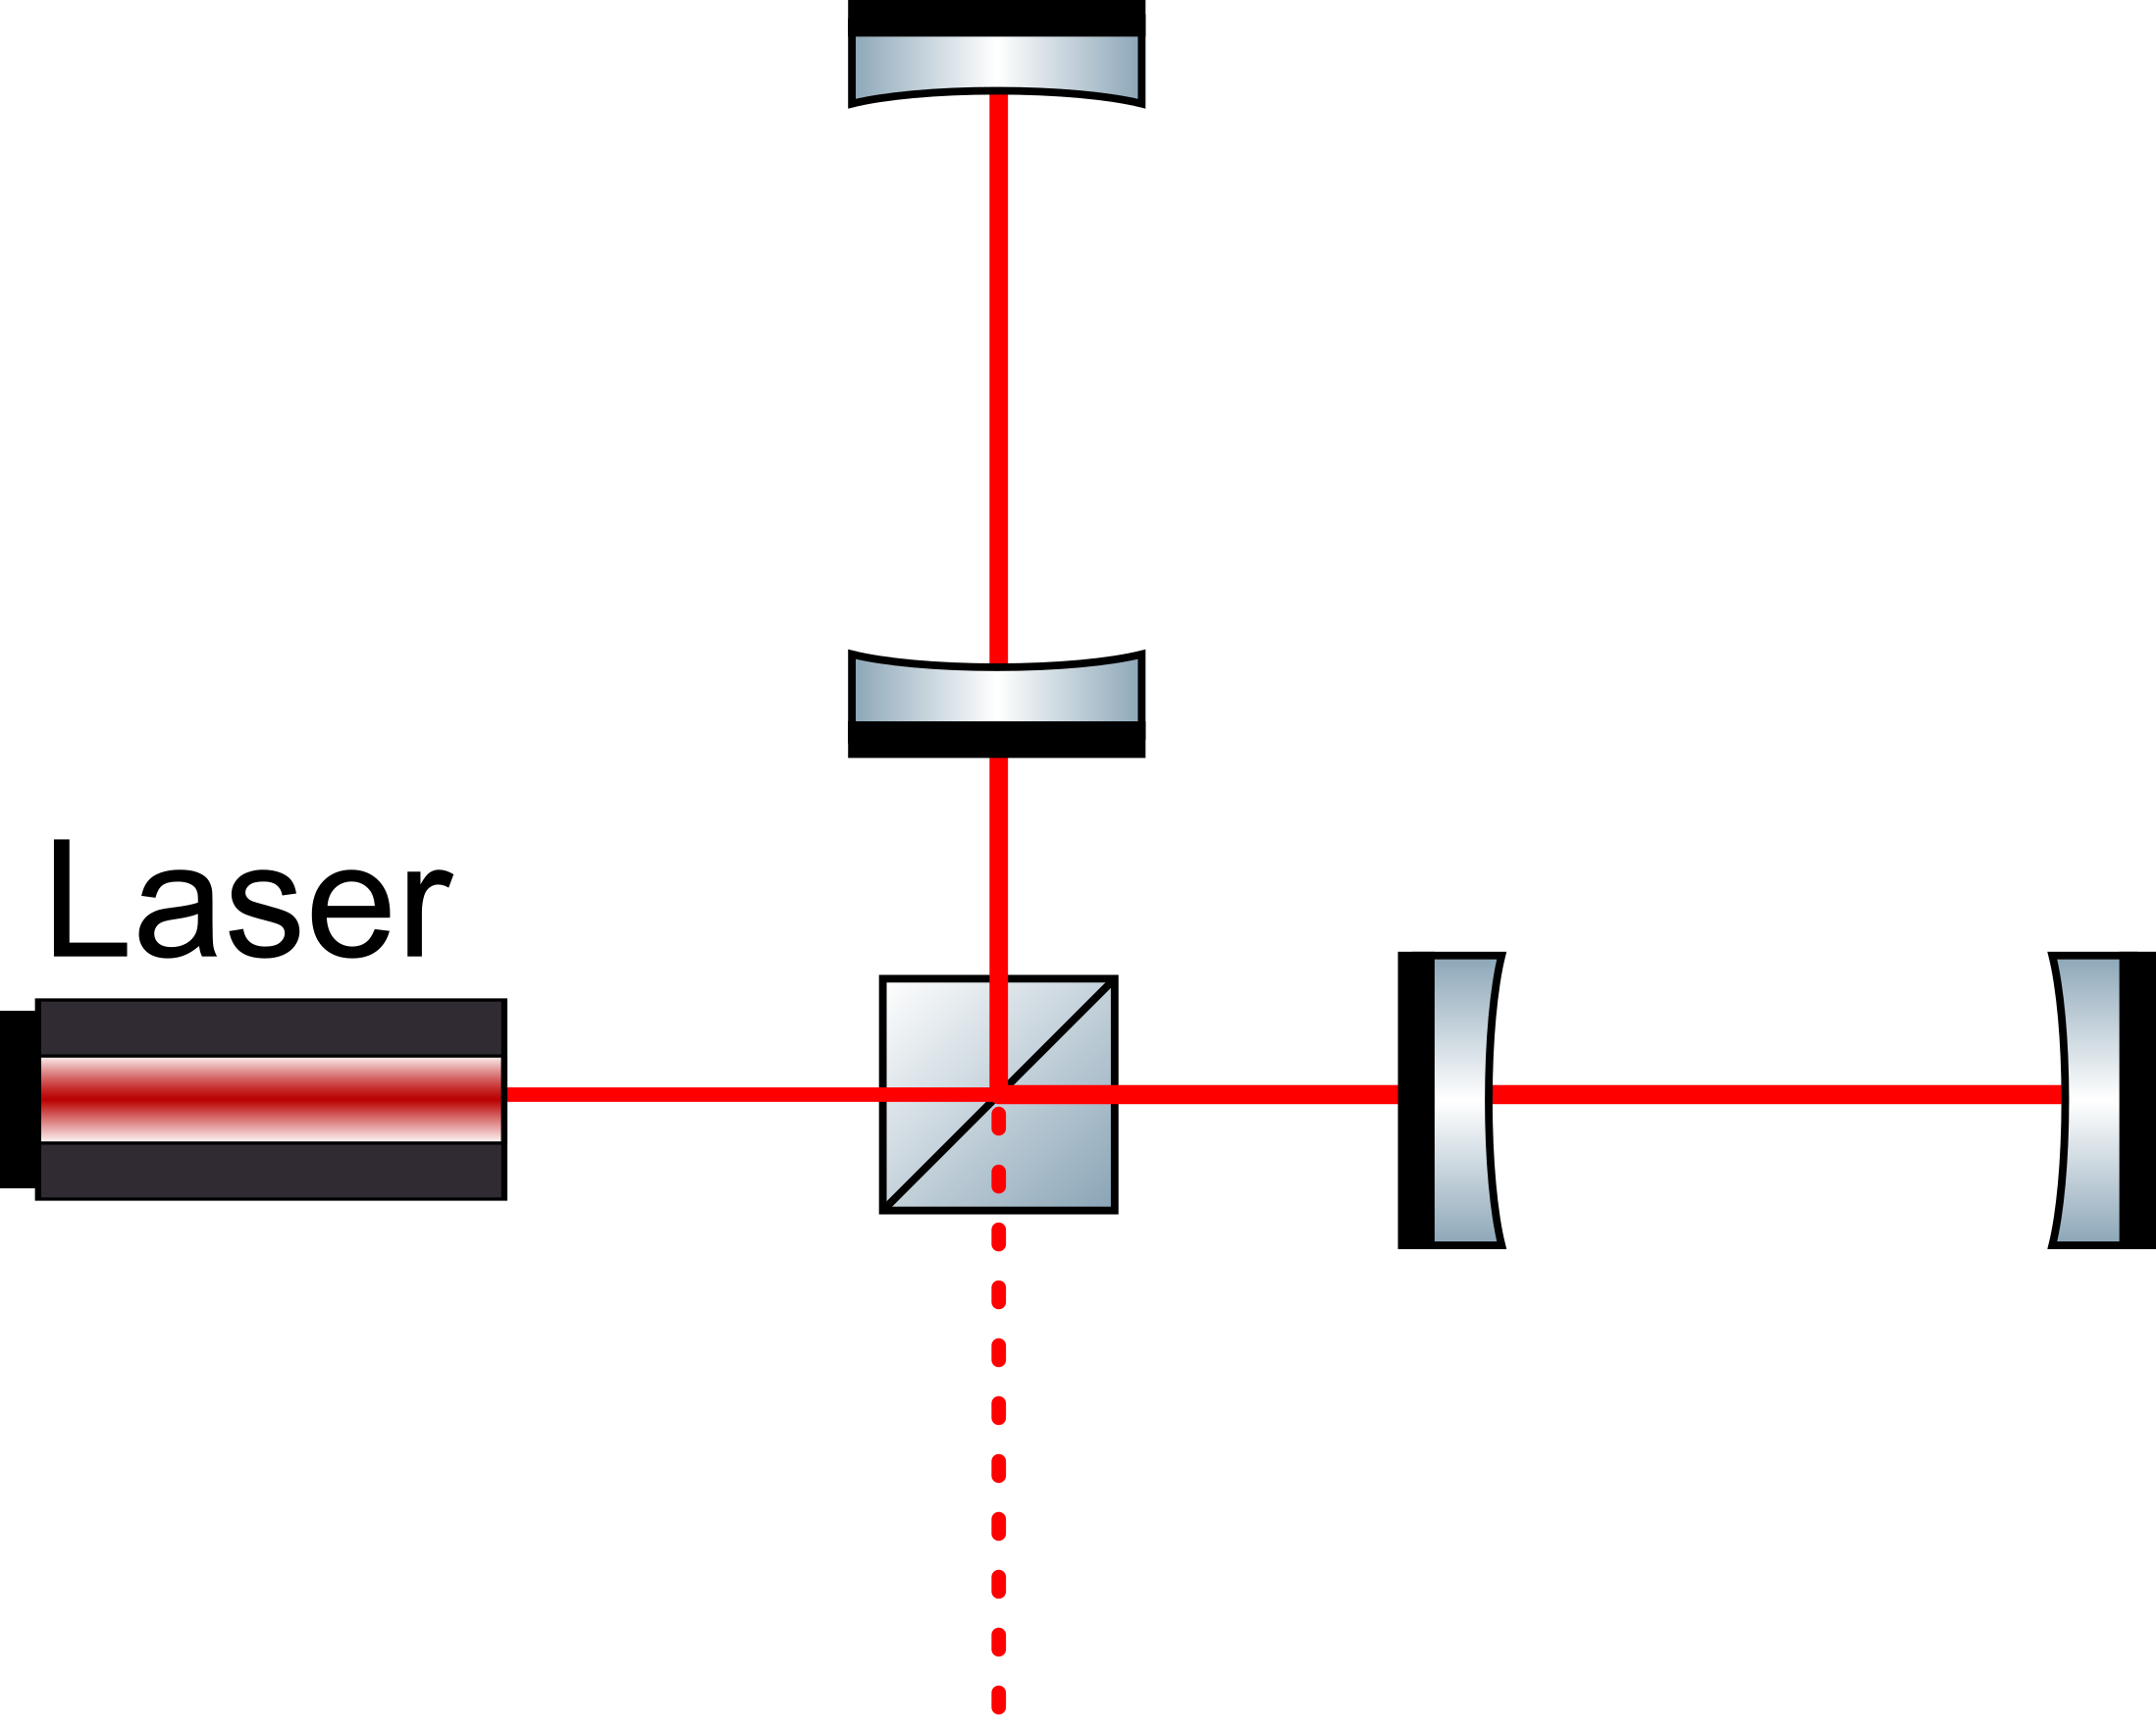
\includegraphics[width=.5 \textwidth]{../Figures/FP_Mich.png}
			\caption{Michelson with Fabry Perot arms}
			\label{fig:FPMichelson}
		\end{figure}
	
		For the carrier field, the amplitude of reflection is simple because the LIGO arms are a strongly over-coupled cavity operating on resonance therefore 
		\begin{equation}
			E(\omega) = \frac{E_0}{\sqrt{2}}  \bigg(-r_1 + \frac{t_1^2 r_2}{1-r_1 r_2} \bigg) \approx -\frac{E_0}{\sqrt{2}}
		\end{equation}
		
		The sidebands are a different story because the modulation caused by the gravitational wave slightly move the field off resonance.  Imagine the carrier circulating in the arms and then suddenly, a disturbance due to a gravitational wave displaces the end mirror at a frequency $\omega_\text{GW}$ by an amount $\Delta L$.   By using the same formalism as the expansion of a modulated field in equation \ref{modE}, the sideband fields can be described by,
		\begin{equation}
		\begin{aligned}\label{Egw}
			E(\pm \omega_{\text{\tiny GW}}) &= \bigg[ \frac{t_1}{1-r_1 r_2 e^{-2ikL}}\bigg] \frac{E_0}{\sqrt{2}} \bigg[\frac{t_1}{1-r_1 r_2 e^{-2i (kL \pm \omega_{\text{\tiny GW}}  \frac{L}{c})}} \bigg] ik\Delta L\\
			& =  \bigg[ \frac{t_1^2}{1-r_1 r_2}\bigg]  \frac{E_0}{\sqrt{2}} \bigg[\frac{ 1}{1-r_1 r_2 e^{-2i  \omega_{\text{\tiny GW}}  \frac{L}{c}}} \bigg] ik\Delta L
		\end{aligned}
		\end{equation}
		The first bracket is the circulating field of the carrier signal amplified by the Fabry Perot cavity and the second bracket is the circulating field slightly off resonance due to the gravitational wave frequency offset.  Setting the fields to resonate already simplifies the equation but it is also reasonable to approximate the gravitational wave as a weak signal and expand the exponential $e^{- 2i \omega_{\text{\tiny GW}}  \frac{L}{c}} \approx 1 - 2i \omega_{\text{\tiny GW}}  \frac{L}{c}$.  This transforms the signal sideband field into a simple form,
		\begin{equation}\label{eq:e_gw}
		E(\pm \omega_{\text{\tiny GW}}) \approx \bigg[\frac{t_1}{1-r_1r_2}\bigg]^2 \, \frac{E_0}{\sqrt{2}} \, \bigg[\frac{1}{1 \pm i \frac{\omega_{\text{\tiny GW}}}{\omega_p}}\bigg] ik\Delta L
		\end{equation}
		where $\omega_p = \frac{1-r_1r_2}{r_1r_2}\frac{c}{2L}$ is the differential pole frequency; notice that it matches the single arm cavity pole.
		
		The photodiode signal at the antisymmetric port is proportional to the beat note between the carrier and signal sideband after demodulation in the audio band with a phase $\phi_{D}$,
		\begin{equation}
		\begin{aligned}
			S &\propto 2 [E(\omega) E^*(+\omega_{\text{\tiny GW}}) +  E(-\omega_{\text{\tiny GW}}) E^*(\omega) ] \sin{(k\delta l)} \sin{(\phi_{D})} \\
			  &\propto E_0^2 \; \frac{8\pi L}{\lambda}  \bigg[\frac{t_1}{1-r_1r_2}\bigg]^2 \bigg[\frac{1}{1 - i \frac{\omega_{\text{\tiny GW}}}{\omega_p}}\bigg] \sin{(k\delta l)} \sin{(\phi_{D})} h_{\text{\tiny GW}}
		\end{aligned}
		\end{equation}
		where the length disturbance $\Delta L$ was transformed to originate from a gravitational wave signal $k \Delta L = \frac{2\pi L}{\lambda} h_{\text{\tiny GW}}$.
		The response of this particular interferometer to differential arm length motion is linearly proportional to the gravitational wave amplitude as well as the input power $P_0 \propto E_0^2$, but there is also a frequency dependent component which is the same as a single Fabry-Perot cavity. This acts like a low pass filter above the corner frequency colloqiually called the darm cavity pole.

		\subsection{Power-Recycled Fabry-Perot Interferometers}
		
		\begin{figure}[ht]
			\centering
			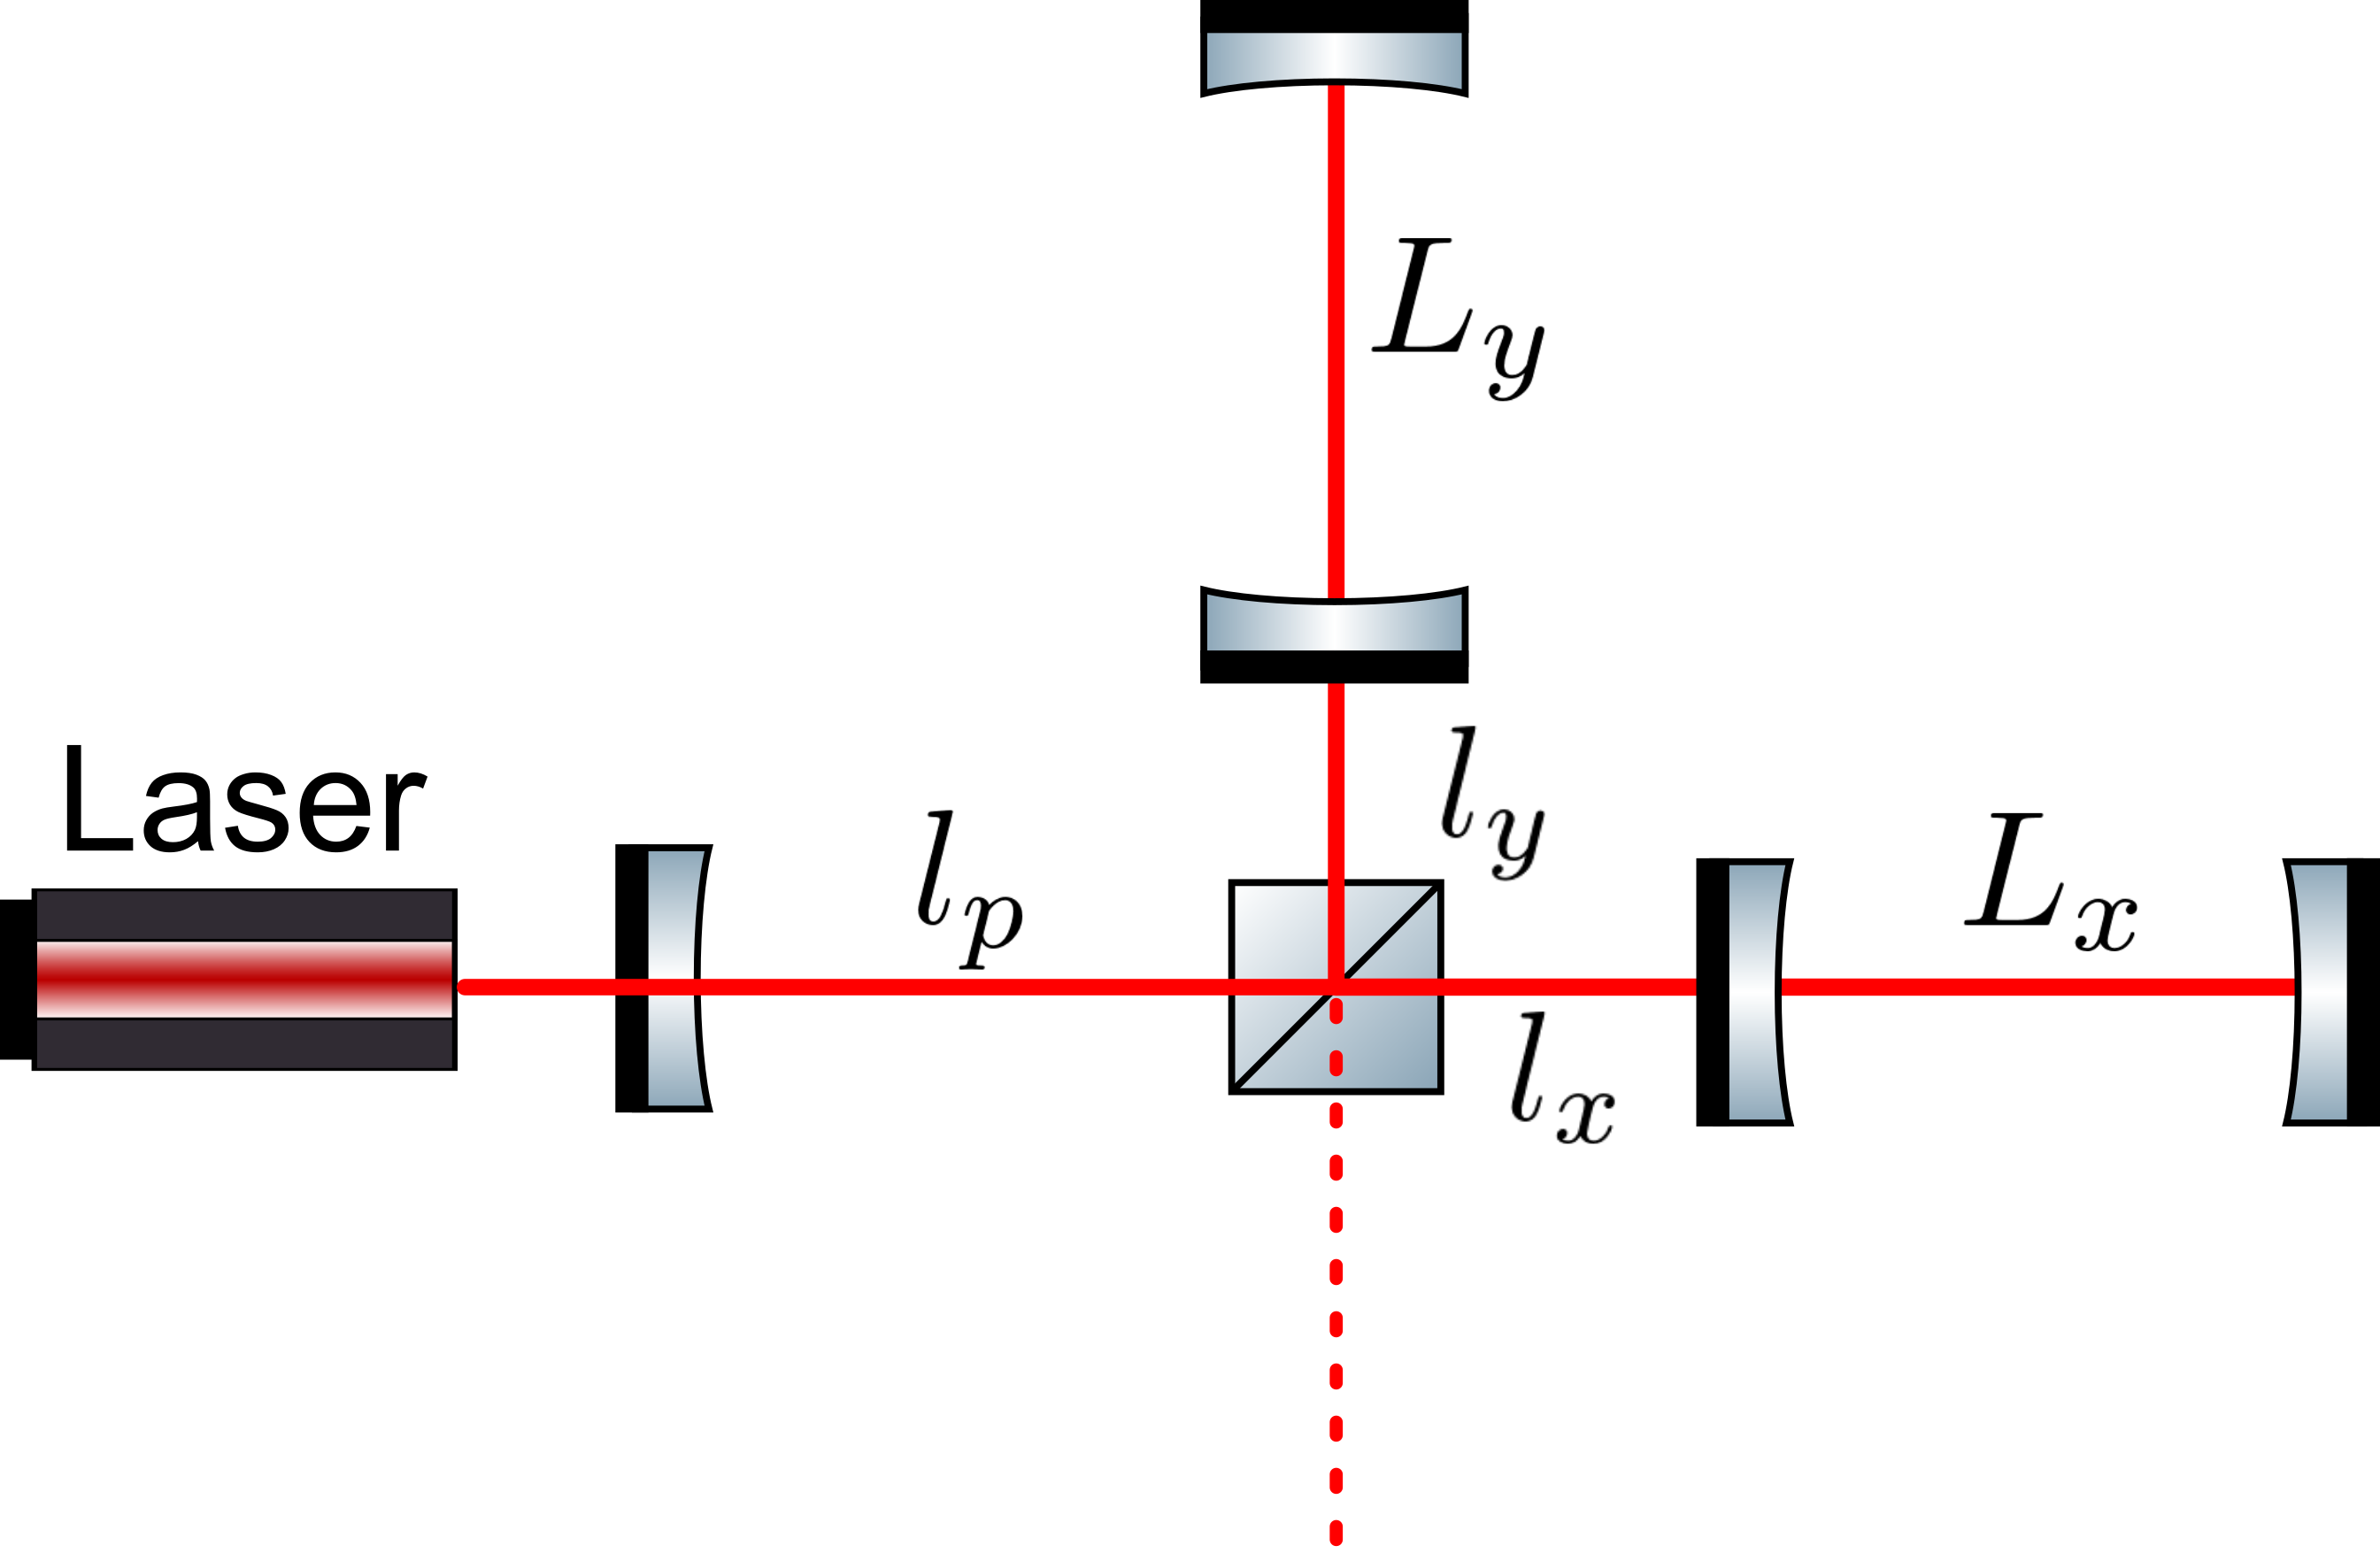
\includegraphics[width=0.5 \textwidth]{../Figures/PRFP_Mich.png}
			\caption[A power recycled Fabry-Perot interferometer.]{\textbf{A power recycled Fabry-Perot interferometer.} Adding a mirror at the symmetric port forms another resonator called the power recycling cavity (PRC) where the distance between from the power recycling mirror (PRM) to the beamsplitter is denoted by $l_p$.  The power recycling cavity can actually be viewed as two linear cavities with the PRM making a cavity with each ITM. }
			\label{fig:PRFPMich}
		\end{figure}

		If the interferometer is operating such that the intensity at the antisymmetric port is close to null, conservation of energy requires that the arm powers will reflect back towards the input laser.  Fritschel et al \cite{Fritschel_Readout} \cite{FritschelLightRecycling} showed the effects of adding a partially reflecting mirror to increase the Michaelson optical gain for both the sideband and carrier fields.
		
		Section \ref{FPmich} showed that the Michelson interferometer with Fabry Perot arms can be represented by a single cavity response.  Therefore it is useful to model a power recycled interferometer by using a coupled cavity approach where the input mirror is replaced with the reflected field of the Michelson on a bright fringe.  Here the reflectivity and transitivity of the power recycling mirror (PRM) is denoted by $r_p$ and $t_p$, respectively.  
		
		In this configuration, the effective length of the cavity is the average path between the power recycling mirror and the high reflectivity surfaces of the input test masses,
		\begin{equation}
		l_{\text{PRC}} = l_\text{p} + \frac{l_x + l_y}{2}
		\end{equation}
		The circulating power in the cavity is given by equation \ref{c_FP} but uses the reflectivity of arm cavities,
		\begin{equation}
		E_{\text{PRC}} = \frac{t_p}{1- r_p r_{\text{FPM}}   e^{-2ik l_{\text{PRC}}}}E_{\text{in}}
		\end{equation}
		where $r_{\text{FPM}}\approx 1 - \frac{\mathbb{F}}{\pi} \mathcal{L}_{\text{ARM}}$ for high finesse cavities and the round trip arm cavity losses are denoted by $\mathcal{L}_{\text{ARM}}$. This is a valid approximation for the advanced LIGO arm cavities since their values for finesse can be around 250 or higher depending on the losses.  This means the circulating power in the recycling cavity while on resonance can be expressed by
		\begin{equation}
		P_{\text{PRC}} = \frac{1-r_p^2}{\bigg[ 1 - r_p  (1 - \frac{\mathbb{F}}{\pi} \mathcal{L}_{\text{ARM}})   \bigg]^2}P_{\text{in}}
		\end{equation} 
		By taking the derivative with respect to $r_p$ and setting to zero, the optimal power recycling tuning is linearly proportional to the round trip loss,
		\begin{equation}
		r_{\text{opt}}  = 1 - \frac{\mathbb{F}}{\pi}\mathcal{L}_{\text{ARM}}
		\end{equation}
		so it important to keep the arm cavity losses as low as possible and this also limits the ability to increase the finesse.
		
		Adding a power recycling mirror will be equivalent to introducing higher power into the arm cavities but it will not shape the gravitational wave sideband frequency dependence in any other way.  This can be reasoned qualitatively by imagining the signal sidebands that get created in the arm cavities and propagate to the beam splitter where they will combine, however, the stretching and squeezing from the gravitational wave pattern will make the x-arm shorter while lengthening the y-arm and vice versa.  This makes the anti-symmetric port transmissive to the signal sidebands but the carrier field which mostly gets reflected to the symmetric port will see the power recycling amplification.  This means the beat note between the static carrier field and gravitational wave signal for a power recycled Fabry-Perot interferometer is
		\begin{equation}
		S_{\text{PRFP}} \propto E_0^2 \; \frac{8\pi L}{\lambda} \sqrt{g_{\text{PRC}}} \bigg[\frac{t_1}{1-r_1r_2}\bigg]^2 \bigg[\frac{1}{1 - i \frac{\omega_{\text{\tiny GW}}}{\omega_p}}\bigg] \sin{(k\delta l)} \sin{(\phi_{D})} h_{\text{\tiny GW}}
		\end{equation}
		where $g_{\text{PRC}} = P_{\text{PRC}}/P_{\text{in}}$ is the power recycling gain.
		
		\subsection{Dual-Recycled Fabry-Perot Interferometers}\label{sec:DRMI}
		
				\begin{figure}[ht]
			\centering
			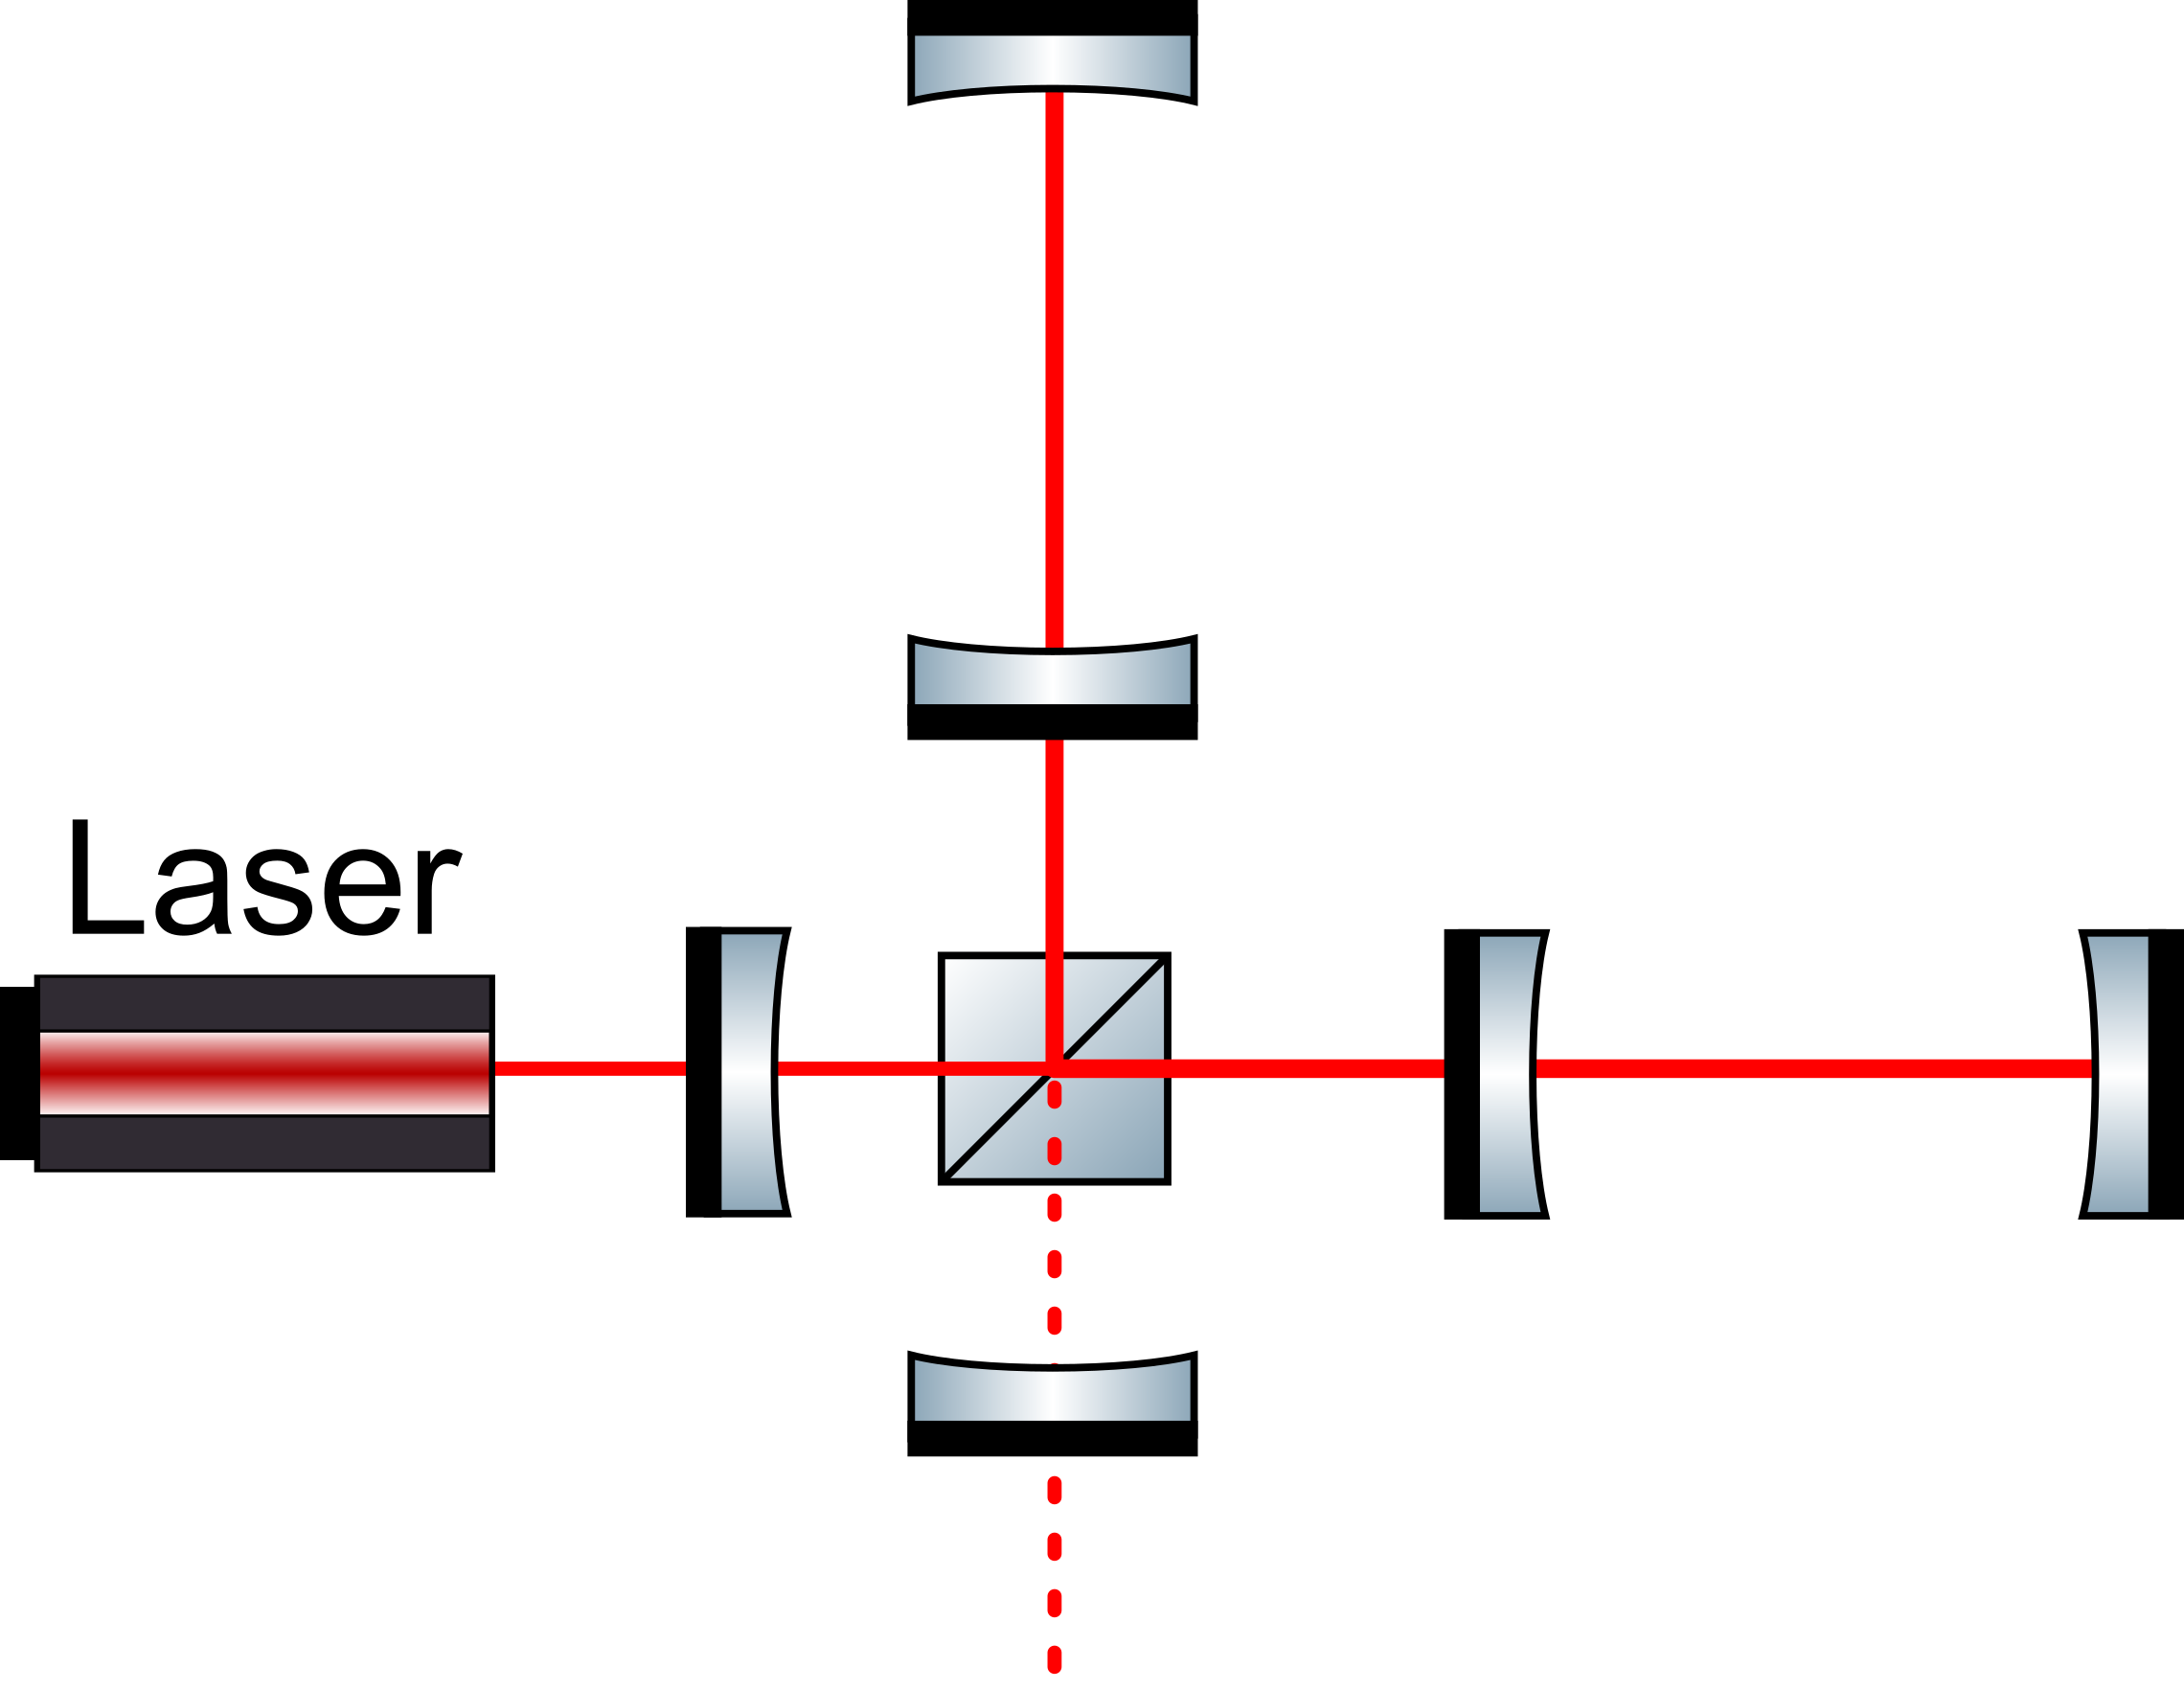
\includegraphics[width=0.5 \textwidth]{../Figures/DRFP_Mich.png}
			\caption[A dual recycled Fabry-Perot interferometer.]{\textbf{A dual recycled Fabry-Perot interferometer.} Adding a signal recycling mirror (SRM) at the anti-symmetric port will change how the gravitational wave signal is read.  Similar to the power recycling cavity, adding a mirror at the output port will create a resonator with the input test masses.}
			\label{fig:DRFPMich}
		\end{figure}
		
		One of the biggest changes made between initial and advanced LIGO was the addition of a signal recycling mirror at the antisymmetric port (Figure \ref{fig:DRFPMich} ). In the previous section, it was shown that the gravitational wave sensitivity was improved by adding a power recycling cavity to increase the effective input power into the Fabry-Perot cavities.  Adding another partially reflecting optic called the signal recycling mirror (SRM) at the antisymmetric port to create a resonant cavity will shape the interferometer's response to gravitational waves.  This allows for some flexibility in optimizing the instrument for specific sources such as binary neutron stars, but it also creates a more broadband response at higher frequencies while allowing the arm cavity finesse and/or power recycling to impart more power.
		
		\begin{figure}[ht]
			\centering
			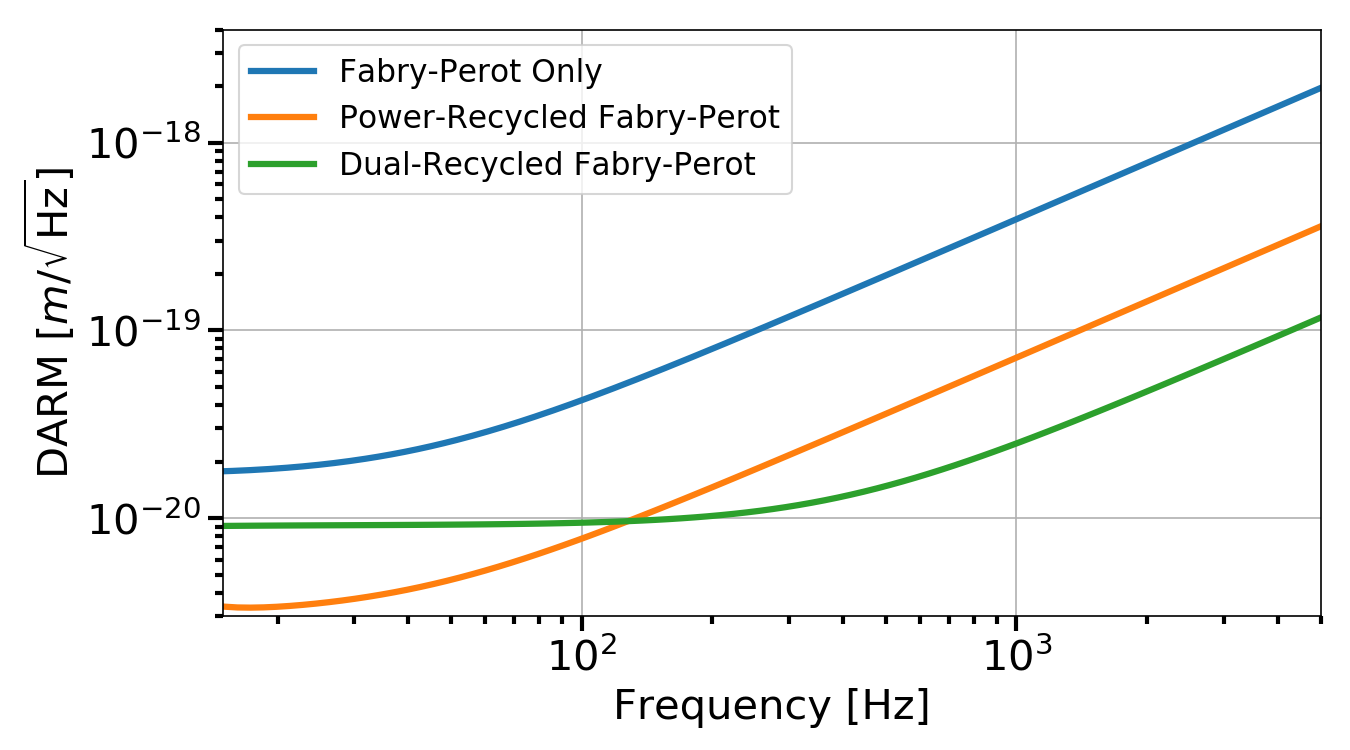
\includegraphics[width=1.0 \textwidth]{../Figures/SN_Lim_Sense.png}
			\caption{Shot noise limited sensitivity}
			\label{fig:SN_sense}
		\end{figure}
		
		\begin{figure}[ht]
			\centering
			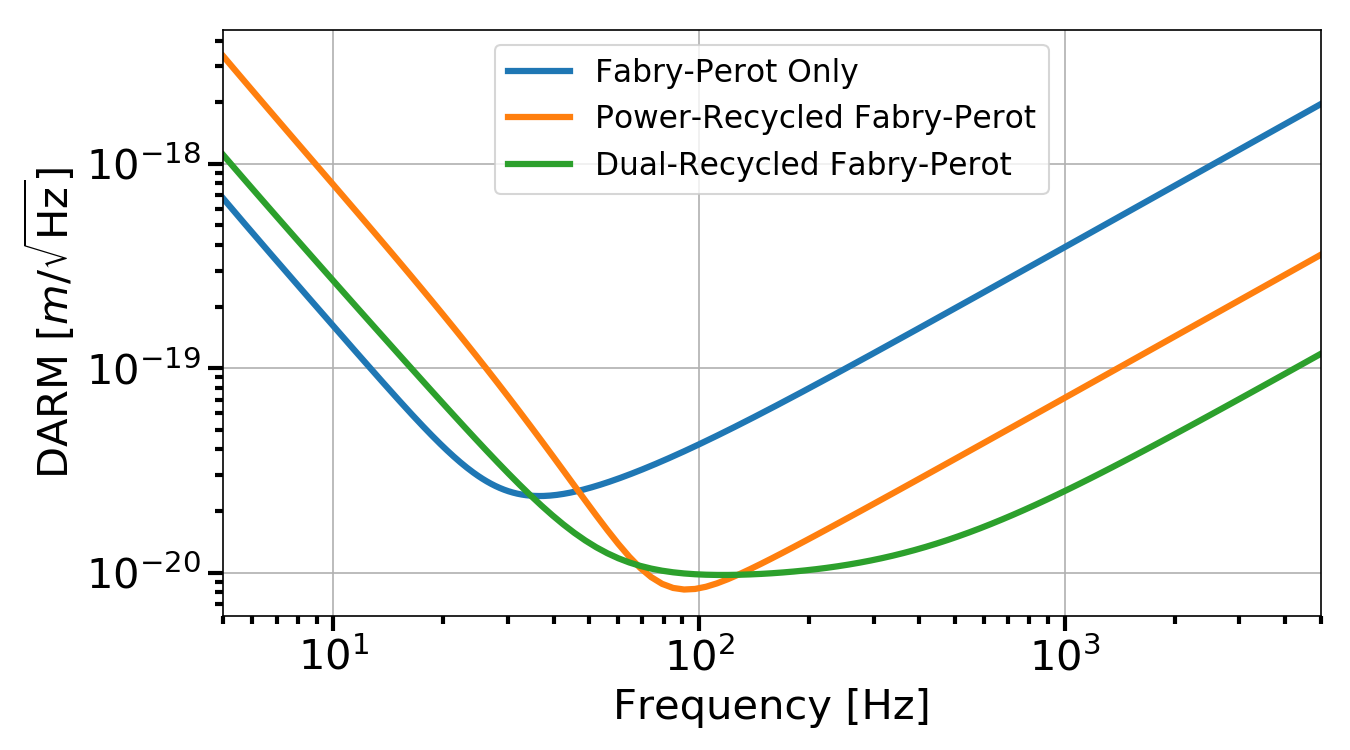
\includegraphics[width=1.0 \textwidth]{../Figures/QM_Limited_Sense.png}
			\caption{Quantum limited sensitivity by combining shot noise and radiation pressure}
			\label{fig:DRMICH_sense}
		\end{figure}
		
		A nice way to model the effect of signal recycling on the gravitational wave sidebands is to combine the SRM and  arm cavity input test mass to create a combined  mirror that is dependent on the round trip phase, $\phi_s$ of the signal recycling cavity.  The SRM will have a reflectivity and transmissivity equal to $r_s$ and $t_s$, respectively, so the combined mirror will have a reflectivity and transmissivity equal to
		\begin{equation}
		r_{1+s} = \frac{r_1 - r_s e^{-2i\phi_s}}{1- r_1 r_s e^{-2i\phi_s}}
		\end{equation}
		\begin{equation}
		t_{1+s} = \frac{t_1 t_s e^{i\phi_s}}{1- r_1 r_s e^{-2i\phi_s}}
		\end{equation}
		where $\phi_s = k \big( l_\text{s} + \frac{l_x + l_y}{2} \big)	$ is the average signal recycling length.
		Plugging this into equation \ref{Egw} in place of the input test mass reflectivity shows that the cavity pole is directly affected by the signal recycling properties, namely, the SRM reflectivity and the microscopic detuning of the length. The field propagating to the true antisymmetric port is in transmission of the signal recycling cavity which is accounted for with the last bracketed term. 
		\begin{equation}
		\begin{aligned}
		E_{\text{AS}}(\pm \omega_{\text{\tiny GW}}) & =  \bigg[ \frac{t_1^2}{1-r_1 r_2}\bigg]  \frac{E_0}{\sqrt{2}} \bigg[\frac{ 1}{1 \pm r_{1+s} r_2 e^{-2i  \omega_{\text{\tiny GW}}  \frac{L}{c}}} \bigg] \bigg[\frac{t_1 t_s e^{i\phi_s}}{1- r_1 r_s e^{-2i\phi_s}}\bigg] ik\Delta L\\
		& \propto \bigg[ \frac{ \text{Constant}}{1 \pm 2 i \frac{r_{1+s} r_2}{1- r_{1+s} r_2}  \omega_{\text{\tiny GW}}  \frac{L}{c}}  \bigg]\\
		& \propto \bigg[\frac{\text{Constant}}{1 \pm i \omega_{\text{\tiny GW}}/\omega_{\text{DR}}}\bigg]
		\end{aligned}
		\end{equation}
		Here, the frequency dependence of the differential cavity pole with dual recycling is denoted by
		\begin{equation}
		\begin{aligned}\label{eq:darm_cav_pole}
			\omega_{\text{DR}} 	&=	\frac{1-r_{1+s}r_2}{r_{1+s}r_2}\frac{c}{2L}\\
								&=	\frac{1- r_1r_s e^{-2i\phi_s} }{ (r_1 - r_s e^{-2i\phi_s})r_2} - 1
		\end{aligned}
		\end{equation}
		
		Figure[ifoconfigs]
		The carrier field will also see a gain from the signal recycling cavity equal to
		\begin{equation}
		\sqrt{g_{\text{SRC}}} = \frac{t_s}{1+ r_s r_{\text{FPM}}   e^{-2i\phi_s}}
		\end{equation}
		It is clear from the equations above that the gravitational wave sideband and carrier fields will see the signal recycling cavity effects differently and the responses are highly sensitive to the length detuning of $\phi_s$.
		Putting all the pieces together to get the dual recycled Fabry-Perot interferometer response to gravitational waves,
		\begin{equation}
		S_{\text{DRFP}} \propto E_0^2 \; \frac{8\pi L}{\lambda} \sqrt{g_{\text{PRC}}}\;\sqrt{g_{\text{SRC}}}\; g_{\text{ARM}} \bigg[\frac{1}{1 - i \frac{\omega_{\text{\tiny GW}}}{\omega_{\text{DR}}}}\bigg] \sin{(k\delta l)} \sin{(\phi_{D})} h_{\text{\tiny GW}}
		\end{equation}

		The previous sections only considered the effect of Fabry-Perot cavities and recycling mirrors at the antisymmetric port (AS) due to the differential length change (DARM) of the 4 kilometer arms but the Advanced LIGO interferometer has a few lengths which are actively controlled. The other degrees of freedom include the common arm length (CARM), the power recycling length (PRCL), and signal recycling length(SRCL).  These signals are sensitive at ports other than AS, such as in reflection of PRM (REFL) and a pick off port in the power recycling cavity (POP).  A good reference for what signals are expected at these important readout points can be found in \cite{kiwamu_freq1} \cite{kiwamu_freq2} \cite{kiwamu_freq3}
		
		\subsection{Fundamental Noise Sources}\label{funnoise}
		The proceeding sections describe ways to increase the response of LIGO to gravitational waves; equally as important is the science of characterizing and reducing the noise contributions from everything that is not gravitational waves to optimize the sensitivity.
		
		\subsubsection{Quantum Noise}\label{Sec:QuantumNoise}
		Virtually all undergraduate quantum mechanics textbooks include a section on the harmonic oscillator [\cite{Shankar}].  A particularly interesting result when solving the Schrödinger equation using creation ($\hat{a^{\dagger}}$) and annihilation $\hat{a}$ operators is the existence of a non-zero energy ground state which has variances in momentum and position related by the Heisenberg uncertainty principle.  When it comes to electromagnetic fields, the pair associated with the uncertainty principle is the amplitude and phase of the laser beam.
		
		As a result, one of the main noise sources that is limiting LIGO's sensitivity comes from the fluctuations of quantum vacuum entering the anti-symmetric port and coupling to the input laser. A quantum mechanical description of an interferometer was constructed by Caves \cite{CavesQMNoise}\cite{Caves2photon} \cite{CavesOscillator}, where he used electric field operators to show that vacuum fluctuations are the cause of radiation pressure and shot noise in a simple interferometer (no resonant cavities).  The following analysis below will also be simplified in this way but is reasonably close in estimating the amount radiation pressure and shot noise.  For studies that take into account more complicated interferometer configurations with resonant cavities refer to Buonanno and Chen \cite{BuonannoChenQMNoise} \cite{ChenQND}.  In general, there has been an explosion of research efforts associated with lowering the noise contributions from vacuum fluctuations \cite{KimbleConversion}.
		
		\textbf{Quantum states}:
		It is well known in physics \cite{Shankar} \cite{Griffiths} that a solution to the quantum harmonic oscillator in the energy eigenbasis employs the annihilation and creation  operators, $\hat{a}^{\dagger}$ and $\hat{a}$, to factorize the Hamiltonian
		\begin{equation}
		\hat{H} = \hbar w (\hat{N} + 1/2)
		\end{equation} 
		where $\hat{N} = \hat{a}^{\dagger}  \hat{a}$ is the number operator.  When using this formalism to create a coherent electromagnetic field, it is useful to define a unitary operator that displaces the vacuum state \cite{GerryKnight}:
		\begin{equation}
		\hat{D} \equiv \hat{D}(\alpha) \equiv \text{exp}(\alpha \hat{a}^{\dagger} - \alpha^{*} \hat{a} ) = e^{-\frac{\vert{\alpha}\vert^2}{2}} e^{\alpha \hat{a}^{\dagger} } e^{\alpha^{*} \hat{a} }
		\end{equation}
		and has the properties,
		\begin{equation}
		\begin{aligned}
		\hat{D}(\alpha) = \hat{D}^{-1}&(\alpha) = \hat{D}(-\alpha)\\
		\hat{D}^\dagger&\, \hat{a} 		\,\hat{D}			= \hat{a} + \alpha \\ 
		\hat{D}^\dagger&\, \hat{a}^\dagger \,\hat{D} 		= \hat{a}^\dagger + \alpha^*
		\end{aligned}
		\end{equation}
		
		When applying the displacement operation on the vacuum state, the resultant vector has an amplitude $\alpha$ and follows the same uncertainty distribution as an unperturbed vacuum vector as shown in Figure[StickandBall],
		\begin{equation}
		\ket{\alpha} = \hat{D} \ket{0} =  e^{-\frac{\vert{\alpha}\vert^2}{2}} e^{\alpha \hat{a}^{\dagger} } \ket{0}
		\end{equation}
		
		\textbf{Radiation Pressure}
		
		One might naively think that power fluctuations in the main laser causes radiation pressure effects on the test masses which will result in noise.  However, if the 50/50 beamsplitter is perfect, then the momentum transfer to each test mass will result in a common length change and will not vary the intensity at the antisymmetric port (or the symmetric port for that matter).  However, the baseline laser power will be important when considering a full quantum mechanical picture of radiation pressure.
		
		Consider plane wave waves entering the interferometer from both the symmetric and anti-symmetric ports.  This method is similar to the input-output methods of section \ref{michelson}, however, the difference being that the beamsplitter will couple the electric fields from the input laser and quantum vacuum.
		
		The electric fields combine at the beamsplitter from both ports and add linearly,
		\begin{subequations}\label{exey}
		\begin{equation}
		E_x = \frac{1}{\sqrt{2}} \bigg[ iE_0 +   E_{AS,in} \bigg]
		\end{equation}
		\begin{equation}
		E_y = \frac{1}{\sqrt{2}} \bigg[  E_0 + i E_{AS,in} \bigg]
		\end{equation}
		\end{subequations}
		where $E_0$ is the input field from the laser and $E_{AS,in}$ is the field from the anti-symmetric port.  The electric fields will travel down each arm and strike the mirrors with intensities denoted by,
		\begin{subequations}
		\begin{equation}
		\vert E_x \vert^2 = \frac{1}{2} \bigg[ \vert E_0 \vert^2 + \vert E_{AS,in} \vert^2  + i(E_0 E^*_{AS,in} - E_0^*E_{AS,in} )\bigg]
		\end{equation}
		\begin{equation}
		\vert E_y \vert^2 = \frac{1}{2} \bigg[ \vert E_0 \vert^2 + \vert E_{AS,in} \vert^2  - i(E_0 E^*_{AS,in} - E_0^*E_{AS,in} )\bigg]`
		\end{equation}
		\end{subequations}
		
		Therefore, differential momentum transfer between the two masses will be equal to the differences in intensities between the two arms:
		\begin{equation}\label{momentumtranfer}
		\begin{aligned}
		 \mathbf{P} 	&= \frac{2 \hbar \omega}{c} \bigg( \vert E_x \vert^2 - \vert E_y \vert^2 \bigg) \\
						&= \frac{2 \hbar \omega}{c} \bigg( E_0 E^*_{AS,in} - E_0^*E_{AS,in} \bigg)\\
		\Rightarrow	\mathbf{\hat{P}}&= \frac{2 \hbar \omega}{c} \bigg( \hat{a}_1^{\dagger} \hat{a}_2 - \hat{a}_2^{\dagger} \hat{a}_1 \bigg)
		\end{aligned}
		\end{equation}
		The last part of equation \ref{momentumtranfer} replaces the classical electric fields with creation and annihilation operators for the symmetric input mode ($\hat{a}_1^{\dagger}$, $\hat{a}_1$) and antisymmetric input mode ($\hat{a}_2^{\dagger}$, $\hat{a}_2$) modes. Recall that there is a well established convention denoting the wave function of the two dimensional modes of the quantum harmonic oscillator \cite{GerryKnight}, $\ket{\alpha,\beta}$, where $\alpha$ denotes the input symmetric mode and $\beta$ refers to the input antisymmetric mode:
		\begin{equation}
		\ket{\alpha,0} = \hat{D}_1(\alpha) \ket{0,0}
		\end{equation}
		The interesting results arising from this formulation is the expectation value turns out to be null,
		\begin{equation}
		\langle \mathbf{\hat{P}} \rangle = \bra{\alpha,0} \mathbf{\hat{P}}\ket{\alpha,0} = 0
		\end{equation}
		However, the variance of the momentum transfer is non-zero, 
		\begin{equation} 
		\begin{aligned}
		\Delta \mathbf{P}^2 &= \langle \mathbf{\hat{P}}^2 \rangle  - \langle \mathbf{\hat{P}} \rangle^2 \\
							&= \bigg(\frac{2 \hbar \omega}{c}\bigg)^2 \bra{\alpha,0}  \hat{a}_1^{\dagger}  \hat{a}_2  \hat{a}_1  \hat{a}_2^{\dagger} + \hat{a}_2^{\dagger}  \hat{a}_1  \hat{a}_2  \hat{a}_1^{\dagger}
							- \hat{a}_2^{\dagger}  \hat{a}_1  \hat{a}_1  \hat{a}_2^{\dagger} - \hat{a}_1^{\dagger}  \hat{a}_2  \hat{a}_2  \hat{a}_1^{\dagger} \ket{\alpha,0}\\
							&= \bigg(\frac{2 \hbar \omega}{c}\bigg)^2 \vert \alpha \vert^2
		\end{aligned}
		\end{equation}
		For some time interval $\Delta T$, the input laser power consisting of $\langle N \rangle =\vert\alpha \vert^2$ photons is
		\begin{equation}
		P_{in} = \frac{\hbar \omega}{\Delta T} \vert \alpha \vert^2
		\end{equation}
		To solve for the amplitude spectral density of the displacement, Newton's second law can be applied in the frequency domain
		\begin{equation}
		M (2\pi f)^2 \tilde{x}(f) = \tilde{F}(f) = \frac{\Delta \mathbf{P}}{\Delta T}
		\end{equation}
		Here, the quantum radiation force spectrum, $\tilde{F}(f)$, is actually flat in frequency because the impacting photons have a randomly distributed amplitude but this gives a straightforward pathway to calculate the displacement spectrum ,
		\begin{equation}
		\tilde{x}_{RP}(f) = \sqrt{\frac{\hbar \omega}{\Delta T} P_{\text{in}}} \frac{1}{2Mc (\pi f)^2}
		\end{equation}
		This means the noise spectral density of radiation pressure for an interferometer with a mirror of mass $M=40 $ kg, input power $P_{\text{in}}=125$ Watts, and laser frequency $\lambda=1064$ nm
		\begin{equation}
		\tilde{h}_{RP}(f) = 2.04\times 10^{-20} \frac{1}{f^2} \; \bigg[ \frac{\text{Strain}}{\sqrt{\text{Hz}}}\bigg]
		\end{equation}
		So it is shown that the contribution of quantum radiation pressure in a simple interferometer increases with the square root of the input power.
		
		\textbf{Shot Noise}
		
		Another way that quantum fluctuations at the antisymmetric port can vary the sensitivity is by adding phase noise.  Imagine holding the test masses rigidly such that the only effects on the output light is due to a phase change in the laser light in the arms. By using the same formulation for radiation pressure but propagating the fields back to the beam splitter, equations \ref{exey} will have extra phase that depends on the arm lengths are denoted by $l_x$ and $l_y$ in a simple Michelson interferometer,
		
		\begin{subequations}\label{exeyout}
		\begin{equation}
		E_{x,\text{out}} = \frac{1}{\sqrt{2}} \bigg[ iE_0 +   E_{AS,\text{in}} \bigg] e^{-i2k l_x}
		\end{equation}
		\begin{equation}
		E_{y,\text{out}} = \frac{1}{\sqrt{2}} \bigg[  E_0 + i E_{AS,\text{in}} \bigg] e^{-i2k l_y}
		\end{equation}
		\end{subequations}
		
		Therefore the antisymmetric port field is described by
		\begin{equation}
		\begin{aligned}
		E_{AS,\text{out}} 	&= \frac{1}{\sqrt{2}} (E_{x,\text{out}} + iE_{y,\text{out}})\\
					&= i e^{-ikl_x-ikl_y} \big[\cos(\Delta \phi) E_0 - \sin(\Delta \phi) E_{AS,\text{in}}\big]
		\end{aligned}
		\end{equation}
		where $\Delta \phi = k(l_x-l_y)$ is used for brevity.  The intensity is once again found by squaring the electric field,
		\begin{equation}
		\begin{aligned}
		\mathbf{I}_{AS,\text{out}} 		&= \vert E_{AS,\text{out}}\vert^2 \\
									&= \bigg[ \cos^2(\Delta \phi)\vert E_0\vert^2 + \sin^2(\Delta\phi)\vert E_{AS,\text{in}}\vert^2 - \sin(\Delta\phi)\cos(\Delta\phi) \big[E_0 E^*_{AS,\text{in}} + E_0^* E_{AS,\text{in}}\big] \bigg]\\
		\Rightarrow	
		\hat{\mathbf{I}}_{AS,\text{out}} 	&= \bigg[ \cos^2(\Delta \phi)a_1^{\dagger}a_1 + \sin^2(\Delta\phi)a_2^{\dagger}a_2 - \sin(\Delta\phi)\cos(\Delta \phi) \big[a_1^{\dagger}a_2 + a_2^{\dagger}a_1 \big] \bigg]\\	
		\end{aligned}
		\end{equation}
		
		The expectation value for the intensity using an input coherent laser with $\alpha$ and quantum vacuum input at the antisymmetric port is
		\begin{equation}
		\begin{aligned}
		\langle \hat{\mathbf{I}} \rangle 	&= \bra{\alpha,0} \hat{\mathbf{I}}_{AS,\text{out}} \ket{\alpha,0}\\
							&= \cos^2(\Delta \phi) \vert \alpha \vert^2
		\end{aligned}
		\end{equation}
		which matches the classical description of a Michelson output described in section \ref{sec:michelson}. Following the same methods to calculate the radiation pressure, photon number variance is
		\begin{equation} 
		\begin{aligned}
		\Delta \mathbf{I} 	&= \sqrt{\langle \mathbf{\hat{I}}^2 \rangle  - \langle \mathbf{\hat{I}} \rangle^2)} \\
							&= \vert \alpha \vert \big[ \cos^2(\Delta \phi)\ \big] 
		\end{aligned}
		\end{equation}
		In order to cast the variance into an expected phase noise, consider the derivative of the intensity with respect to the phase and plugging in the input power,
		\begin{equation}
		\frac{\partial I}{\partial \phi} = - 2 \vert \alpha \vert^2\cos(\Delta \phi) \sin(\Delta \phi)
		\end{equation}
		\begin{equation}
		\delta \phi = \sqrt{\frac{\hbar \omega}{ P_{\text{in}}}} \cot(\Delta \phi)
		\end{equation}
		Here $\delta \phi$ is the microscopic change in phase due to shot noise, whereas $\Delta\phi$ is the DC offset in the arm lengths to begin with. So in general, the shot noise contribution is dependent on the amount of light present at the anti-symmetric port and this will vary depending on what type of signal readout scheme is implemented.  To calculate the shot noise sensitivity, the phase shift in shot noise can be scaled by a factor of $\frac{\lambda}{2 \pi}\frac{1}{L}$ where $\lambda$ is the laser wavelength and $L$ is the DC length of the Michelson arms,
		\begin{equation}
		\tilde{h}_{SN}(f) = 8.2\times 10^{-22} \; \bigg[ \frac{\text{Strain}}{\sqrt{\text{Hz}}}\bigg]
		\end{equation}
		Unsurprisingly, the shot noise is proportional to $1/\sqrt{P_{\text{in}}}$ and the initial phase difference between the interferometer arms. There are a few subtleties associated with measuring shot noise, this model assumes that the interferometer readout is a single photodetector located at the antisymmetric port.  However,it is possible to measure the light at two different phases (90 degrees apart) and subtract the results to get better averaging.   As shown in section \ref{sec:DRMI}, there is a freedom to choose the readout scheme of the interferometer (heterodyne or homodyne) which will also affect the overall quantum sensitivity and introducing Fabry-Perot cavities will shape the shot noise for frequencies above the differential cavity pole in equations \ref{eq:e_gw} and \ref{eq:darm_cav_pole}.
		
		\subsubsection{Seismic Noise}
		Reference:[Kissel Thesis]
		The main contributions to seismic noise are primarily caused by either natural occurrences  (tectonic plates, wind driven microcosms, oceanic storms etc) or man-made disturbances (heavy automotive traffic, industrial machinery, etc) which contribute to the background hum of motion.  In general, this will be the low frequency barrier for all terrestrial gravitational-wave detectors.  One of the biggest upgrades from eLIGO to aLIGO was the increase in complexity for seismic isolation and suspensions.  Using multiple stages of actively controlled platforms \cite{fabrice_sei1} \cite{fabrice_sei2} \cite{fabrice_strat}\cite{sei_isol}, the noise contribution can be attenuated for frequencies larger than ~1Hz;  in addition, the use of quadruple pendulums to hang the main arm cavity optics further reduces the motion above the pendulum's resonance frequency\cite{driggers_global}\cite{BlairBook}. This is a tremendous upgrade from the mostly passive isolation methods used in initial LIGO.  An interesting point to note is that the estimate of noise contributions from seismic activities to the strain sensitivity is negligible for frequencies above 10 Hz, but absolutely vital for lock acquisition and resonator stability \cite{Hang_LF} \cite{Fritschel_alignment}.
		
		\subsubsection{Thermal Noise}
		Brownian motion \cite{brownian_einstein} is the random movement of particles suspended in a fluid.  The LIGO test masses that make up the 4 kilometer long Fabry-Perot cavities are large macroscopic objects but their constituent atoms can be excited by the ambient temperature which leads to random motion. Those atoms are interconnected which allow for the propagation of an infinite number of elastic wave modes that contain random relative phases and the linear superposition of the modes create distortions that result in thermal noise.	
	
		A good way to start analyzing thermal noise is to consider a simple harmonic oscillator with mass $m$, that is in a thermal bath with a damping force, $F=-b\dot{x}(t)$.
		\begin{equation}
		\ddot{x}(t) + \gamma \dot{x}(t) + \omega_{0}^2 x(t) = F/m
 		\end{equation}
		Here, $\gamma = b/m$ and the force, $F$, can be described by white noise.  In this case, the force represents work being done on the system by the external world whereas the damping factor is the release of the system's energy to the outside world.  By taking the Fourier transform, the equation of motion becomes
		\begin{equation}\label{harmonic}
		\tilde{x}(f) = \frac{\tilde{F}(f)}{m} \; \frac{1}{\omega^2 +i \gamma \omega + \omega_{0}^2} 
		\end{equation}
		This implies that the spectral density for viscous damping is
		\begin{equation}\label{svis}
		S_{Vis} = \frac{S_F}{m^2} \; \frac{1}{(\omega^2 -\omega_{0}^2)^2 + (\gamma\omega)^2}
		\end{equation}
		Because the noise is due to a thermal bath, the integrated power over all frequencies must satisfy this equation
		\begin{equation}
		\frac{1}{2} \int_{-\infty}^{\infty} S_{Vis} (\omega) \frac{\text{d}\omega}{2\pi} = \frac{k_B T}{m\omega_{0}^2}
		\end{equation}
		where $k_B$ is the familiar Boltzmann's constant and $T$ is the ambient temperature.  Solving the integral and plugging the result for $S_F$ back into the equation \ref{svis} gives the power spectrum for viscous damping,
		\begin{equation}\label{vis}
		S_{Vis} = \frac{4k_B T \gamma}{m} \frac{1}{(\omega^2 - \omega_{0}^2)^2 + (\gamma\omega)^2}
		\end{equation}
		This equation shows that for three different frequency regimes, the response can vary wildly.
		\begin{subequations}
			\begin{equation}
			\omega<< \omega_{0} \rightarrow S_{vis} = \frac{4k_B T}{m Q \omega_{0}^3}
			\end{equation}
			\begin{equation}
			\omega \approx \omega_{0} \rightarrow S_{vis} = \frac{4k_B T}{m \omega_{0}^3} Q
			\end{equation}
			\begin{equation}
			\omega >> \omega_{0} \rightarrow S_{vis} = \frac{4k_B T}{m Q} \frac{\omega_0}{\omega^4} 
			\end{equation}
		\end{subequations}
		where $Q=\omega_{0}/\gamma$ is commonly known as the quality factor of a resonator.  Qualitatively, this is directly proportional to the resonance height and its thinness.  Figure [visthermalnoise] shows the resultant frequency dependent power spectrum for a few different quality factors, for higher $Q$ systems the amount of noise contribution from thermal noise is reduced at frequencies above the resonance.  Another commonly used definition of the quality factor is the amount of energy loss per cycle, if the $Q$ of a system is high, then the amount of energy loss per oscillation is very small and will take a longer time returning to equilibrium.  A good description of the quality factor and its application to gravitational wave detectors can be found in section 7.5 of \cite{Saulson}.
		
		As system's mode number increases, the previous analysis becomes very difficult to solve analytically. However, the connection between a damped harmonic oscillator's energy loss and power spectrum can be described generically using the Fluctuation Dissipation Theorem,
		\begin{equation}\label{FD}
		S_x(f) = \frac{k_B T}{\pi^2 f^2} \vert \operatorname{\mathbb{R}e} (Y(f)) \vert
		\end{equation}
		where $Y(f)$ is the complex mechanical admittance (inverse of the impedance) of a system. The physical interpretation of equation \ref{FD} can be viewed as a tunnel of energy between a system of interest and the outside world.  If there is an ability to couple energy from one system to another via some process, then the reverse must be true as well. This subtle but powerful statement can be applied generally.  For example, a resistor which is able to dissipate thermal energy when current is flowing through it will convert random external temperature fluctuations into stray currents that results in $Johnson$ $Noise$.  Another principle which the FD theorem relies upon is that when the system is in thermal equilibrium, its response to fluctuations will be the same as applying a small force randomly.
		
		Using this method, the mechanical admittance of a system is defined as $Y(f) = \dot{x}(f)/F(f)$ which can be written down directly for a damped harmonic oscillator using equation \ref{harmonic},
		\begin{equation}
			\begin{aligned}
			\frac{\dot{x}(f)}{F} &= \frac{i \omega}{m} \frac{1}{\omega_{0}^2 - \omega^2 +i\gamma \omega}\\
								 &= \frac{i\omega}{m} \frac{(\omega_{0}^2 - \omega^2 - i \gamma \omega)}{(\omega_0^2 - \omega^2)^2 + (\gamma \omega)^2}
			\end{aligned}
		\end{equation}
		and by plugging this into the fluctuation dissipation theorem, the power spectral density matches equation \ref{vis} for the viscous damping.  To extend the usage further, consider the thermal noise from a solid which has some thermoelastic dissipation from an internal mode given by $F_{diss} = -k(1+\phi_L) x(t) $ where the phase term comes from the lag between applied force and the system's response to said force.  By solving Newton's second law with this new damping term, the displacement spectrum becomes 
		\begin{equation}
		\tilde{x}(f) =  \frac{\tilde{F}}{m} \; \frac{1}{(1 + i\phi_L ) \omega_{0}^2 - \omega^2 }
		\end{equation}
		Unlike the previous example of viscous damping, the integral for thermoelastic dissipation only holds for some frequency regime but implementing the fluctuation dissipation theorem leads directly to the noise power spectrum,
		\begin{equation}
			S_{TD}(f) =  \frac{4k_B T \omega_{0}^2 \phi_L}{m \omega} \frac{1}{(\omega^2 - \omega_{0}^2)^2 + (\omega_{0}\phi_L)^2}
		\end{equation}
		The frequency response will also be different compared to viscoelastic dissipation,
		\begin{subequations}
			\begin{equation}
			\omega<< \omega_{0} \rightarrow S_{vis} = \frac{4k_B T}{m Q \omega \omega_{0}^2}
			\end{equation}
			\begin{equation}
			\omega \approx \omega_{0} \rightarrow S_{vis} = \frac{4k_B T}{m \omega_{0}^3} Q
			\end{equation}
			\begin{equation}
			\omega >> \omega_{0} \rightarrow S_{vis} = \frac{4k_B T}{m Q} \frac{\omega_0^2}{\omega^5} 
			\end{equation}
		\end{subequations}
		The structural damping formalism can also be applied to the suspension fibers which hold the 40 kilogram test masses \cite{SaulsonThermalSus}, \cite{Saulson} which yield a noise spectral density that contains resonances at a variety of frequencies.  The lower two modes consist of the pendulum and rocking modes, while starting at 500 hertz the violin modes will be seen.  In fact, the violin modes and their harmonics could get rung up from earthquakes and saturate the output mode cleaner's DC photodiodes so they must be actively damped in order to obtain nominal low noise.
		
		The largest contribution to the thermal noise for current interferometers do not stem from viscous damping \cite{SaulsonThermalNoise}, thermoelastic damping of the substrate \cite{Saulson}, or internal friction of the suspension fibers, but rather from the thermal noise contributed by the mechanical loss of the dielectric coatings \cite{HarryThermalCoat} \cite{EvansBallmerThermalOptic} which cause phase noise at the high reflectivity surface of the mirrors.
		
		\begin{figure}[ht]
			\centering
			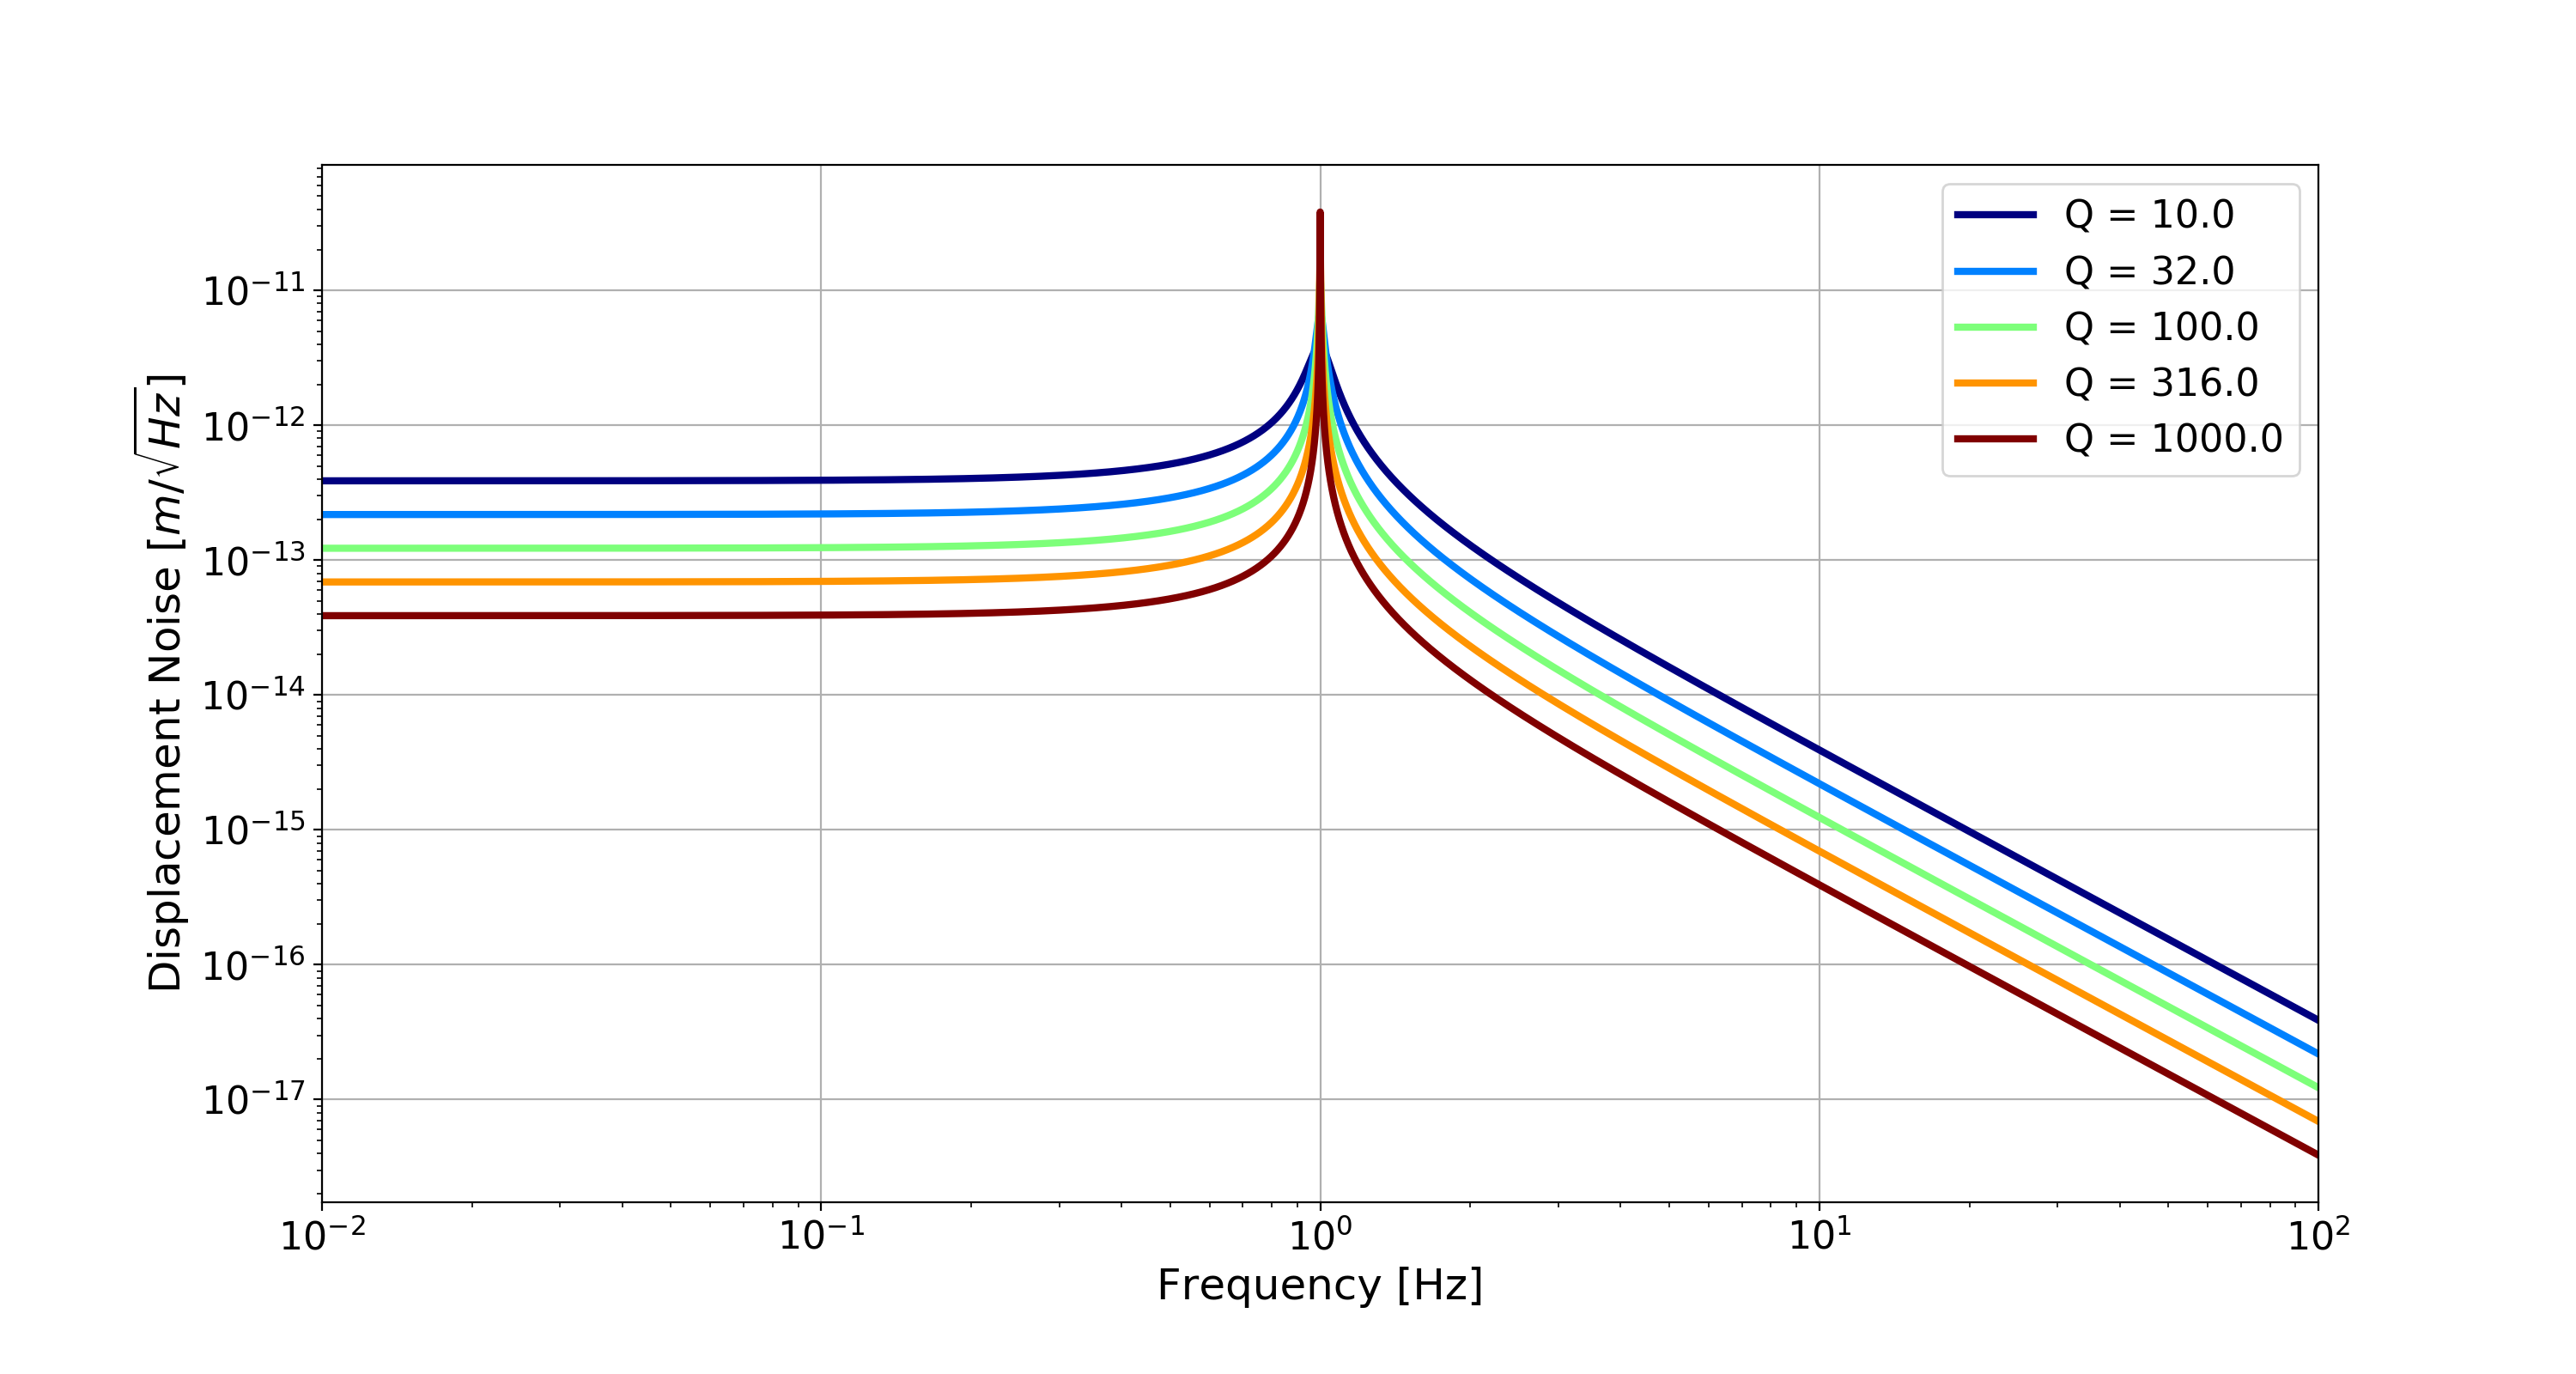
\includegraphics[width=.9 \textwidth]{../Figures/ThermalNoise_ASD.png}
			\caption[Displacement spectrum for thermal noise.]  
			{\textbf{Displacement spectrum for thermal noise.} Adding an extra Q changes the peak and thermal noise above the resonance.}
			\label{fig:ThermalNoise}
		\end{figure}
		
		\subsubsection{Newtonian Noise}
		Described in the previous sections are noise sources which can be reduced using increasingly complicated techniques such as increased isolation stages for seismic or using squeezed states of light for quantum noise.  However, for Newtonian noise caused by fluctuating gravitational fields from the wave motion of the ground \cite{SaulsonNewtonian} and \cite{ThorneNewtonian} is one that cannot easily be reduced but possibly be measured and fed-forward or subtracted off-line \cite{DriggersNewtonian}.

	\section{Mode Matching with Squeezed States of Light}
	In Section \ref{Sec:QuantumNoise}, the quantum limited sensitivity for a Michelson interferometer was shown to be composed of shot noise and radiation pressure. Although quantum fluctuations are a fundamental noise source, their effects can be modified by manipulating the  vacuum state with correlated photons and injecting these states of light into the antisymmetric port of the interferometer.  Within the LIGO community, this procedure of modifying quantum vacuum is called squeezing.  The production of squeezed states with nonlinear devices is a well understood subject and was successfully tested in the sixth LIGO science run \cite{LSCBeyondQM}\cite{LSCEnhancedSenseSqz}.  An extension of the formalism described in Section \ref{Sec:QuantumNoise} was developed by Caves-Schumaker \cite{Caves2photon} which describes two-photon quantum optics and squeezing, but it is outside of the scope in terms of mode matching. 
	
	However, it useful to understand the quantum noise in a way which scales the interferometer sensitivity in terms of the $\textit{Standard Quantum Limit}$ (SQL).   The radiation pressure and shot noise add in quadrature to form the quantum noise and both are proportional to the square root of the input power but in different regimes.  The SQL refers to the input power minimizes the total quantum noise and is the minimum achievable noise without squeezing.  The radiation-pressure back-action coupling constant, $\kappa$, is given by \cite{KimbleConversion}
	\begin{equation}
	\kappa = \frac{4 P_0 \omega_{0}}{m c^2 f^2}
	\end{equation}
	where $P_0$ is the input power on the beamsplitter, $\omega_{0}$ is the laser angular frequency, $m$ is the optic mass, and $f$ is the Fourier domain frequency.  The SQL for a simple Michelson is given by \cite{KimbleConversion},
	\begin{equation}
	S_{SQL} = \frac{4 \hbar}{m L^2 f^2}
	\end{equation}
	With these two equations above, the total single-sided power spectral density for a simple Michelson is
	\begin{equation}
	S_{SM} = \frac{S_{SQL}}{2} \bigg( \frac{1}{\kappa}  + \kappa\bigg)
	\end{equation}
	Here the first term is represents the shot noise while the second term is the radiation pressure contribution. 
	\begin{figure}[ht]
		\centering
		\begin{subfigure}[b]{0.45\textwidth}
			\centering
			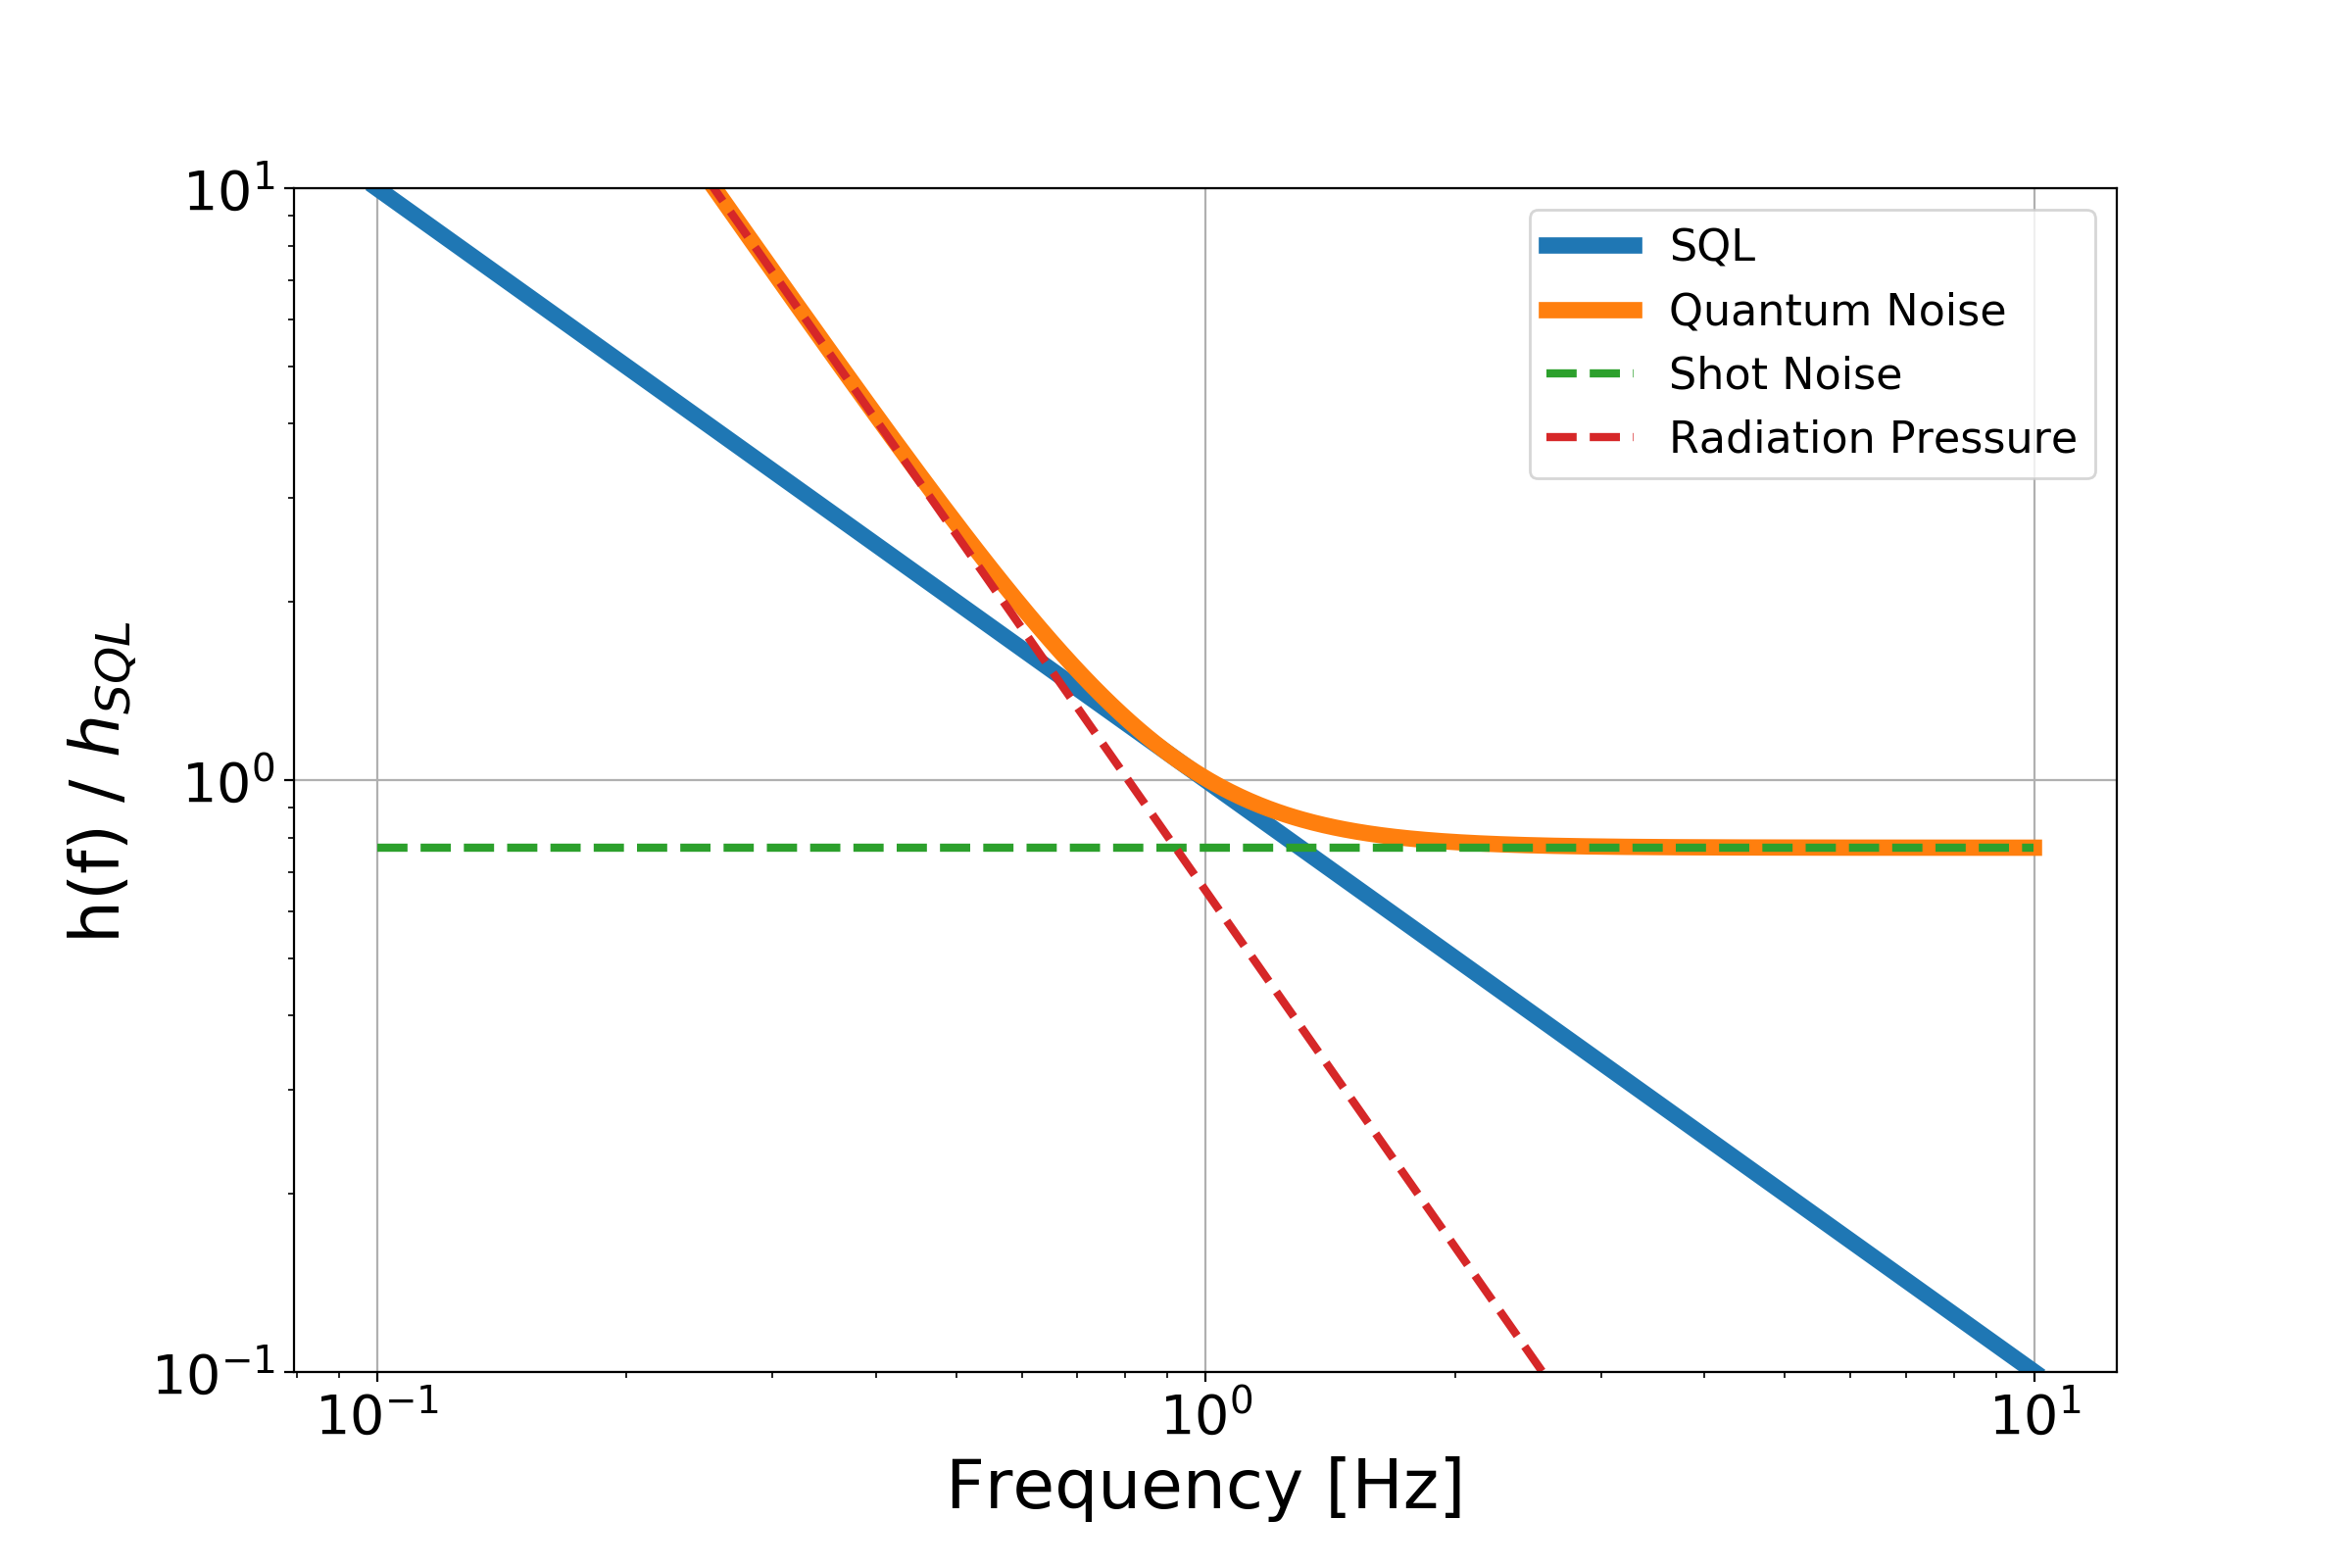
\includegraphics[width=\textwidth]{../Figures/Kimble_SM_QM.png}
			\caption{Simple Michelson quantum noise}
			\label{fig:kimble_SM}
		\end{subfigure}
		\hfill
		\begin{subfigure}[b]{0.45\textwidth}
			\centering
			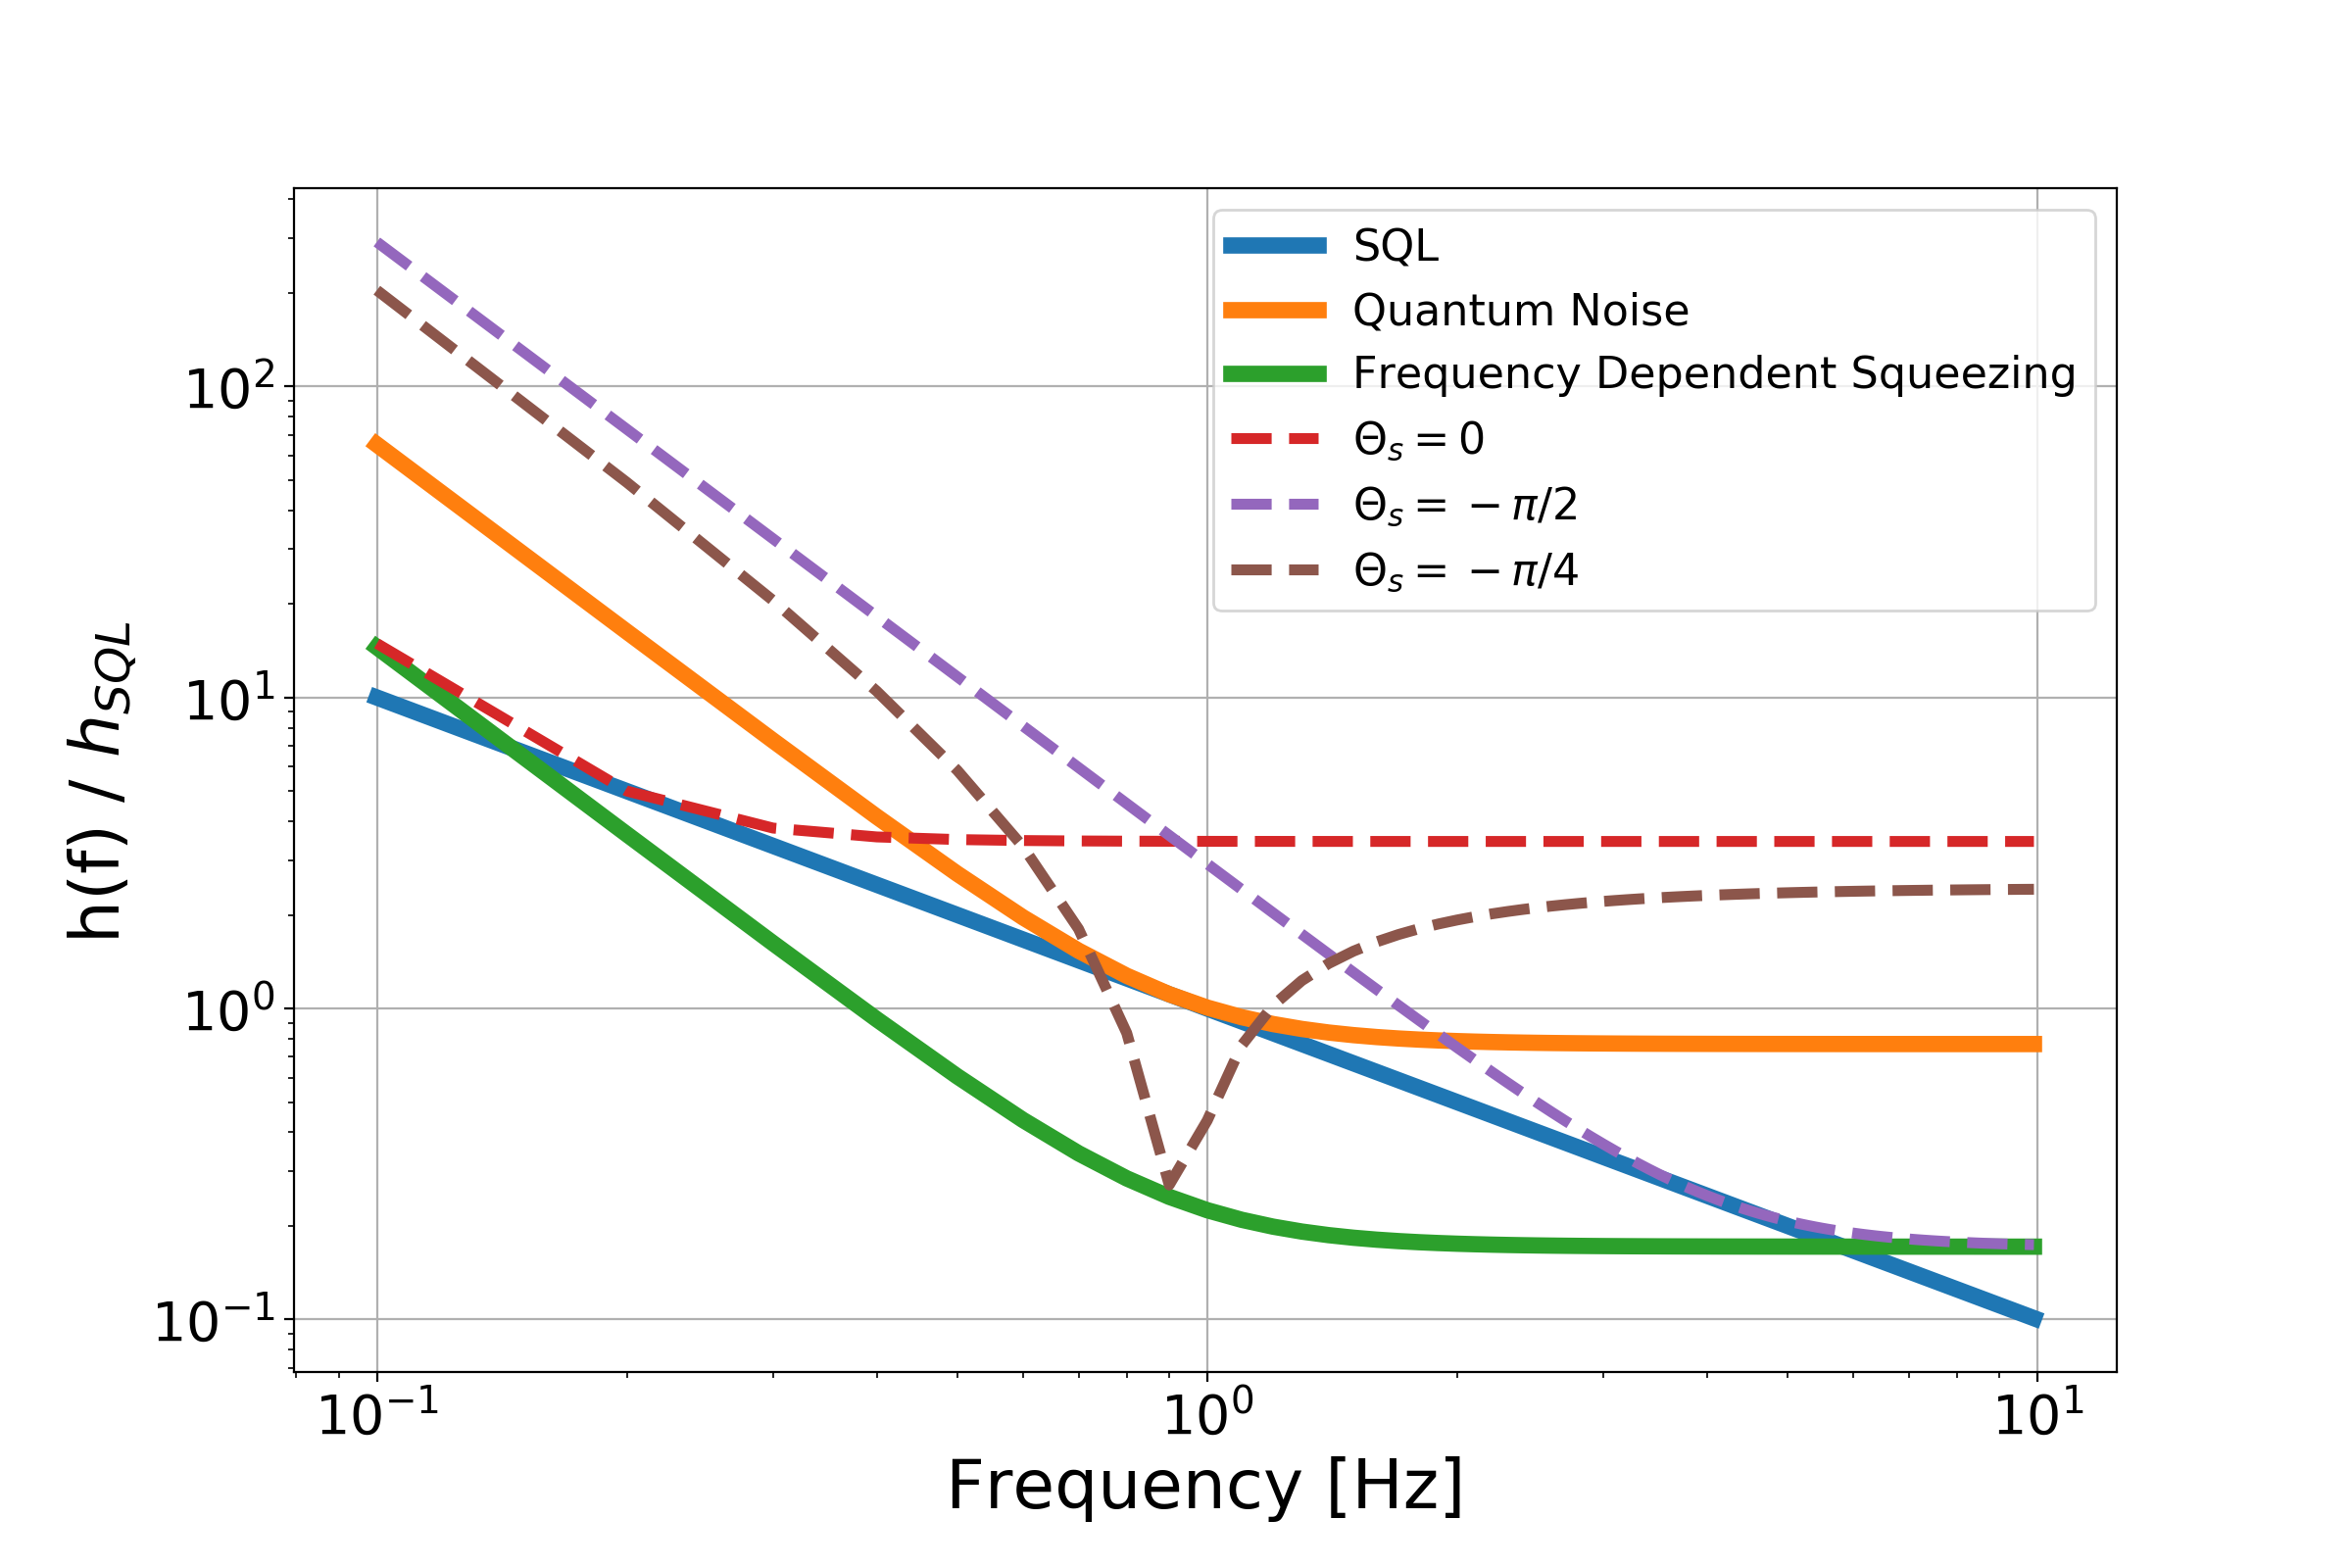
\includegraphics[width=\textwidth]{../Figures/Kimble_SM_QM_sqz.png}
			\caption{Simple Michelson quantum noise with squeezing}
			\label{fig:kimble_SM_sqz}
		\end{subfigure}
		\caption{The amplitude spectral density of gravitational wave strain normalized by the standard quantum limit.}
		\label{fig:PSD_SM}
	\end{figure}
	
	Modifying the field entering the antisymmetric port by replacing the quantum vacuum with a squeezed state has interesting effects on the strain sensitivity and reduces the noise floor below the standard quantum limit. The power spectral density for a simple Michelson with injected squeezing is described by \cite{KimbleConversion}
	\begin{equation}
	\begin{aligned}
	S_{SM Sqz} 	&=  \frac{S_{SQL}}{2} \bigg( \frac{1}{\kappa}  + \kappa\bigg) [\cosh{2R} - \cos(2(\phi_s+\theta_s)) \sinh{2R}]\\
	&= \frac{S_{SQL}}{2} \bigg( \frac{1}{\kappa}  + \kappa\bigg) e^{-2R} \qquad \text{for } \theta_s = -\phi_s
	\end{aligned}
	\end{equation}
	where $R$ is the squeeze factor, $\theta_s$ is the squeeze angle, and $\phi_s = \cot^{-1}(\kappa)$.  The squeeze angle can change the regime of strain which is affected, for example, when injecting for optimal shot noise reduction one would choose $\theta_s=\pi/2$.  However, when trying to reduce the radiation pressure noise, then choosing $\theta_s=0$ is optimal.   For the second line in the equation above, to achieve broadband squeezing, the squeeze angle must be rotated as a function of frequency.  Fortunately, this can be achieved by reflecting the squeezer beam off a filter cavity before injecting into the interferometer \cite{Oelker_FD_sqz} \cite{EvansRealistic}.
	
	\begin{figure}[ht]
		\centering
		\begin{subfigure}[b]{0.7\textwidth}
			\centering
			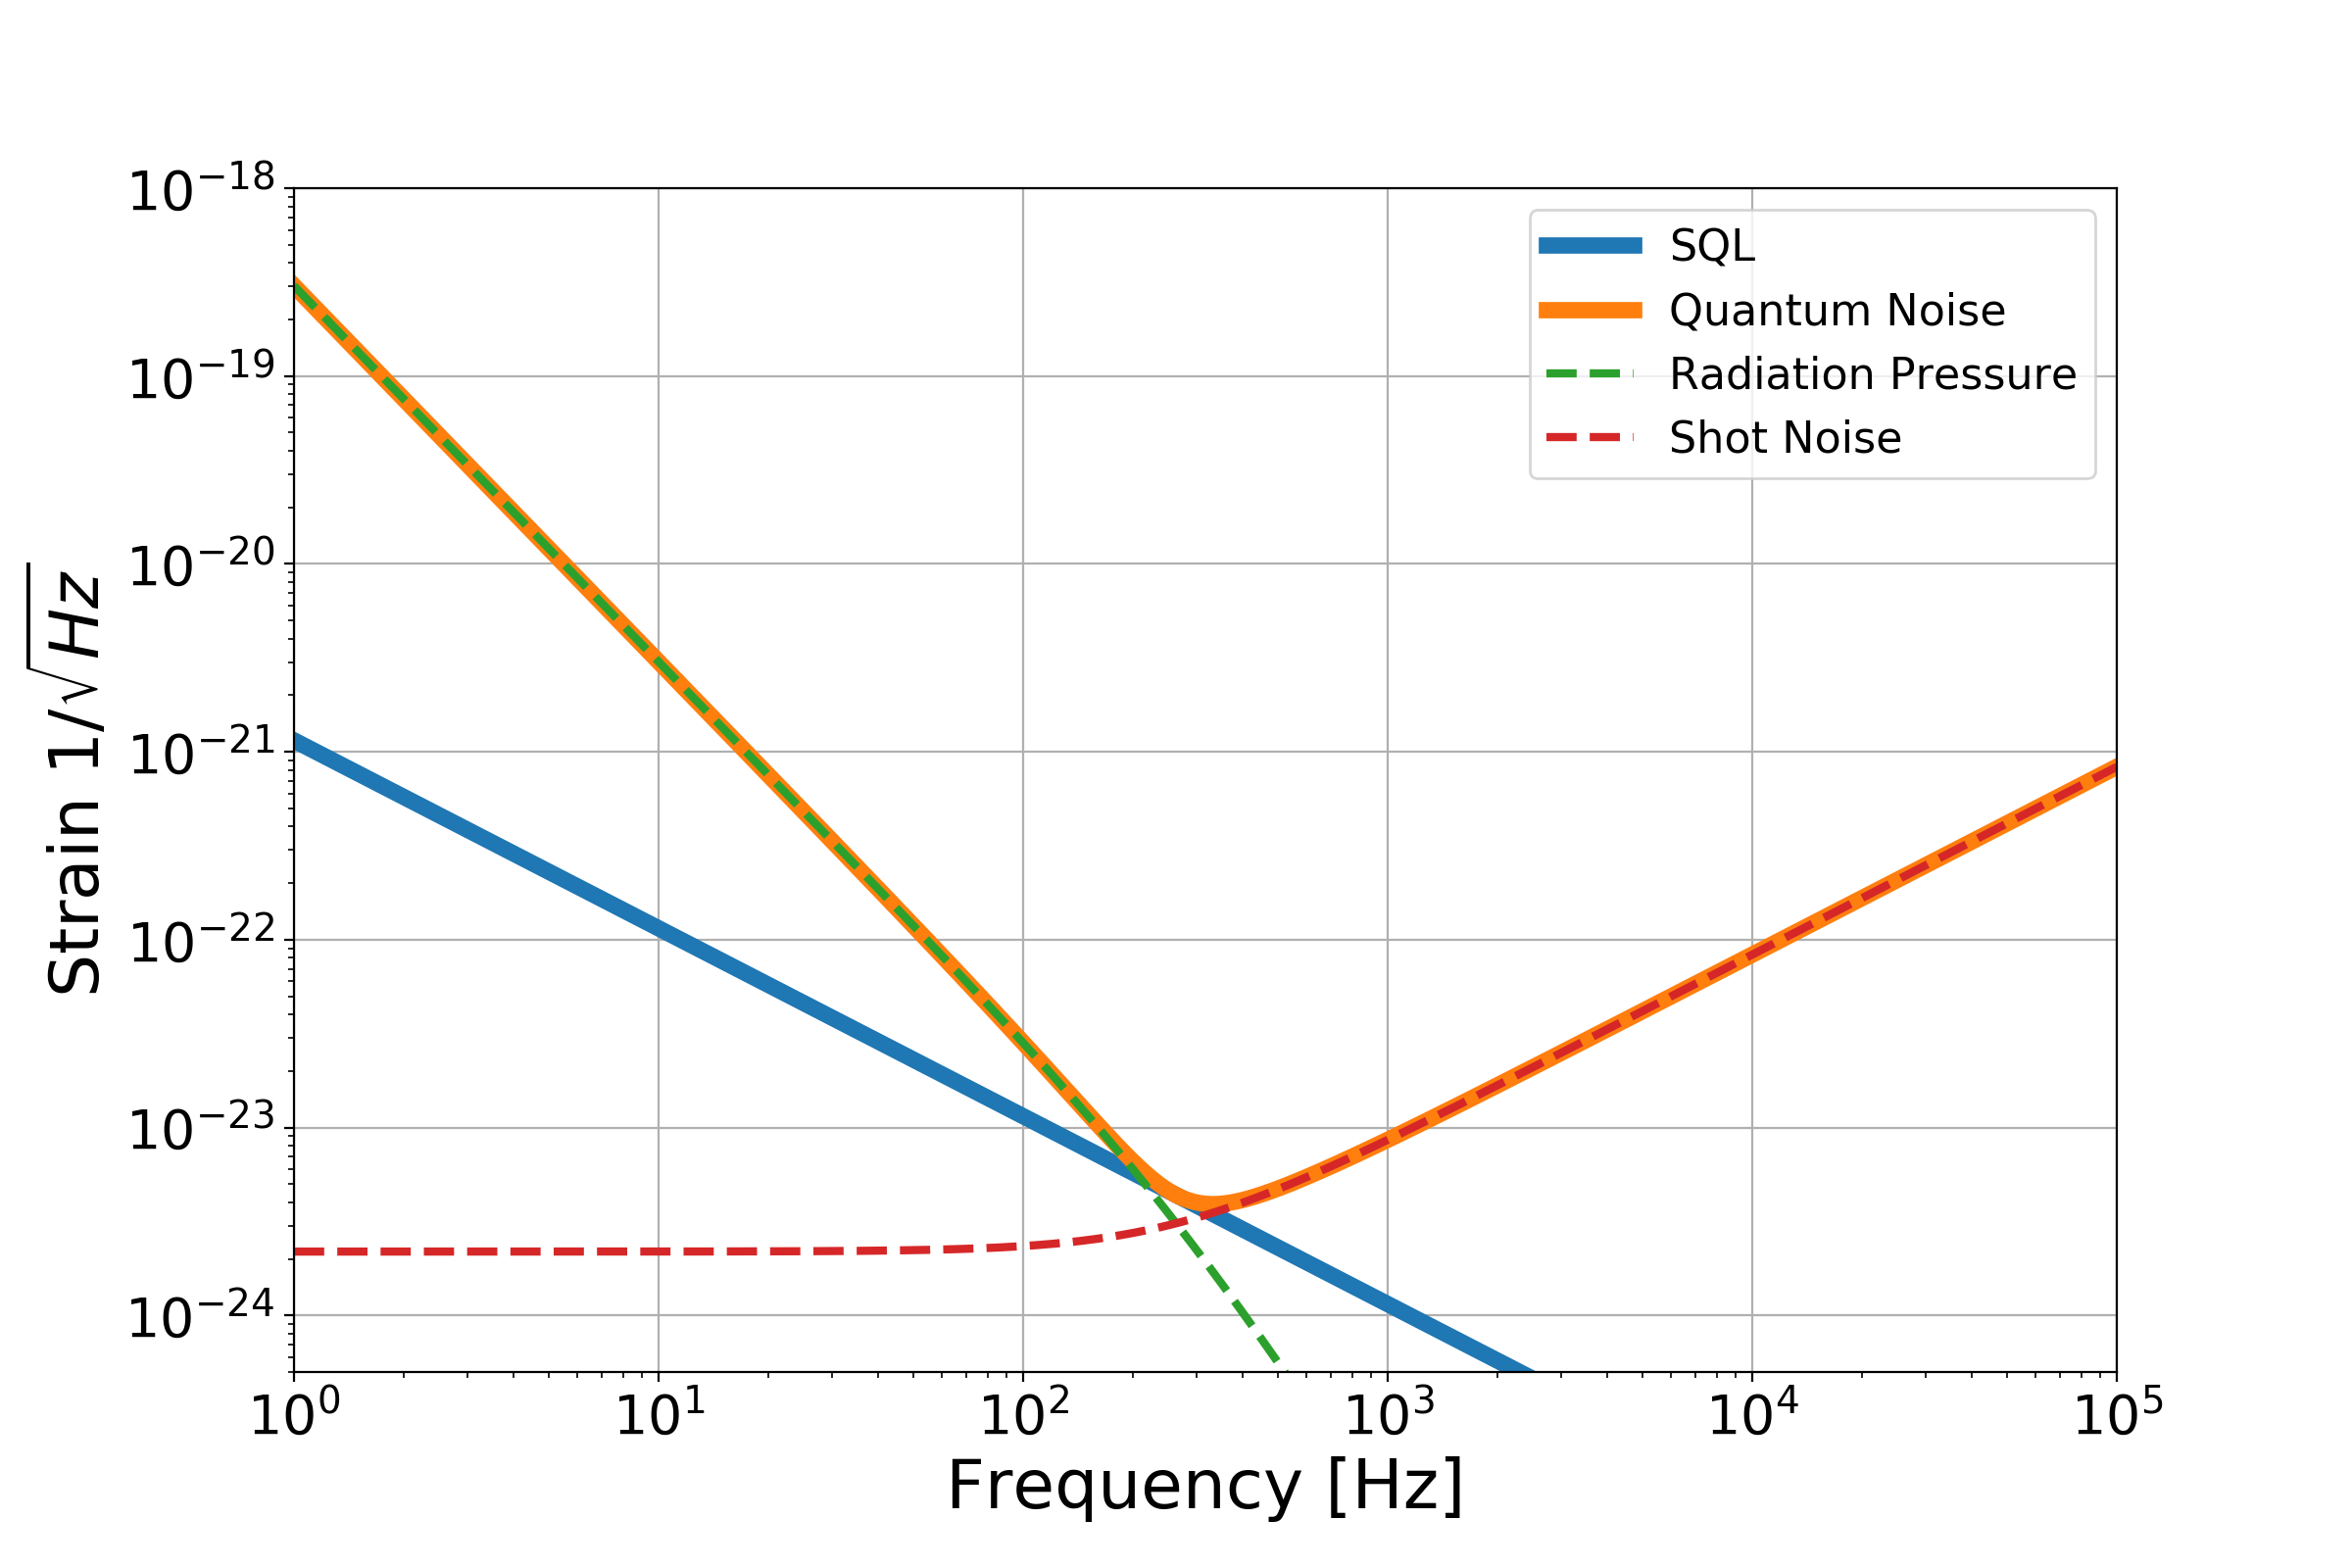
\includegraphics[width=\textwidth]{../Figures/Kimble_PRFPMI_QM.png}
			\caption{Power recycled Fabry Perot Michelson quantum noise}
			\label{fig:kimble_PRFMI}
		\end{subfigure}
		\hfill
		\begin{subfigure}[b]{0.7\textwidth}
			\centering
			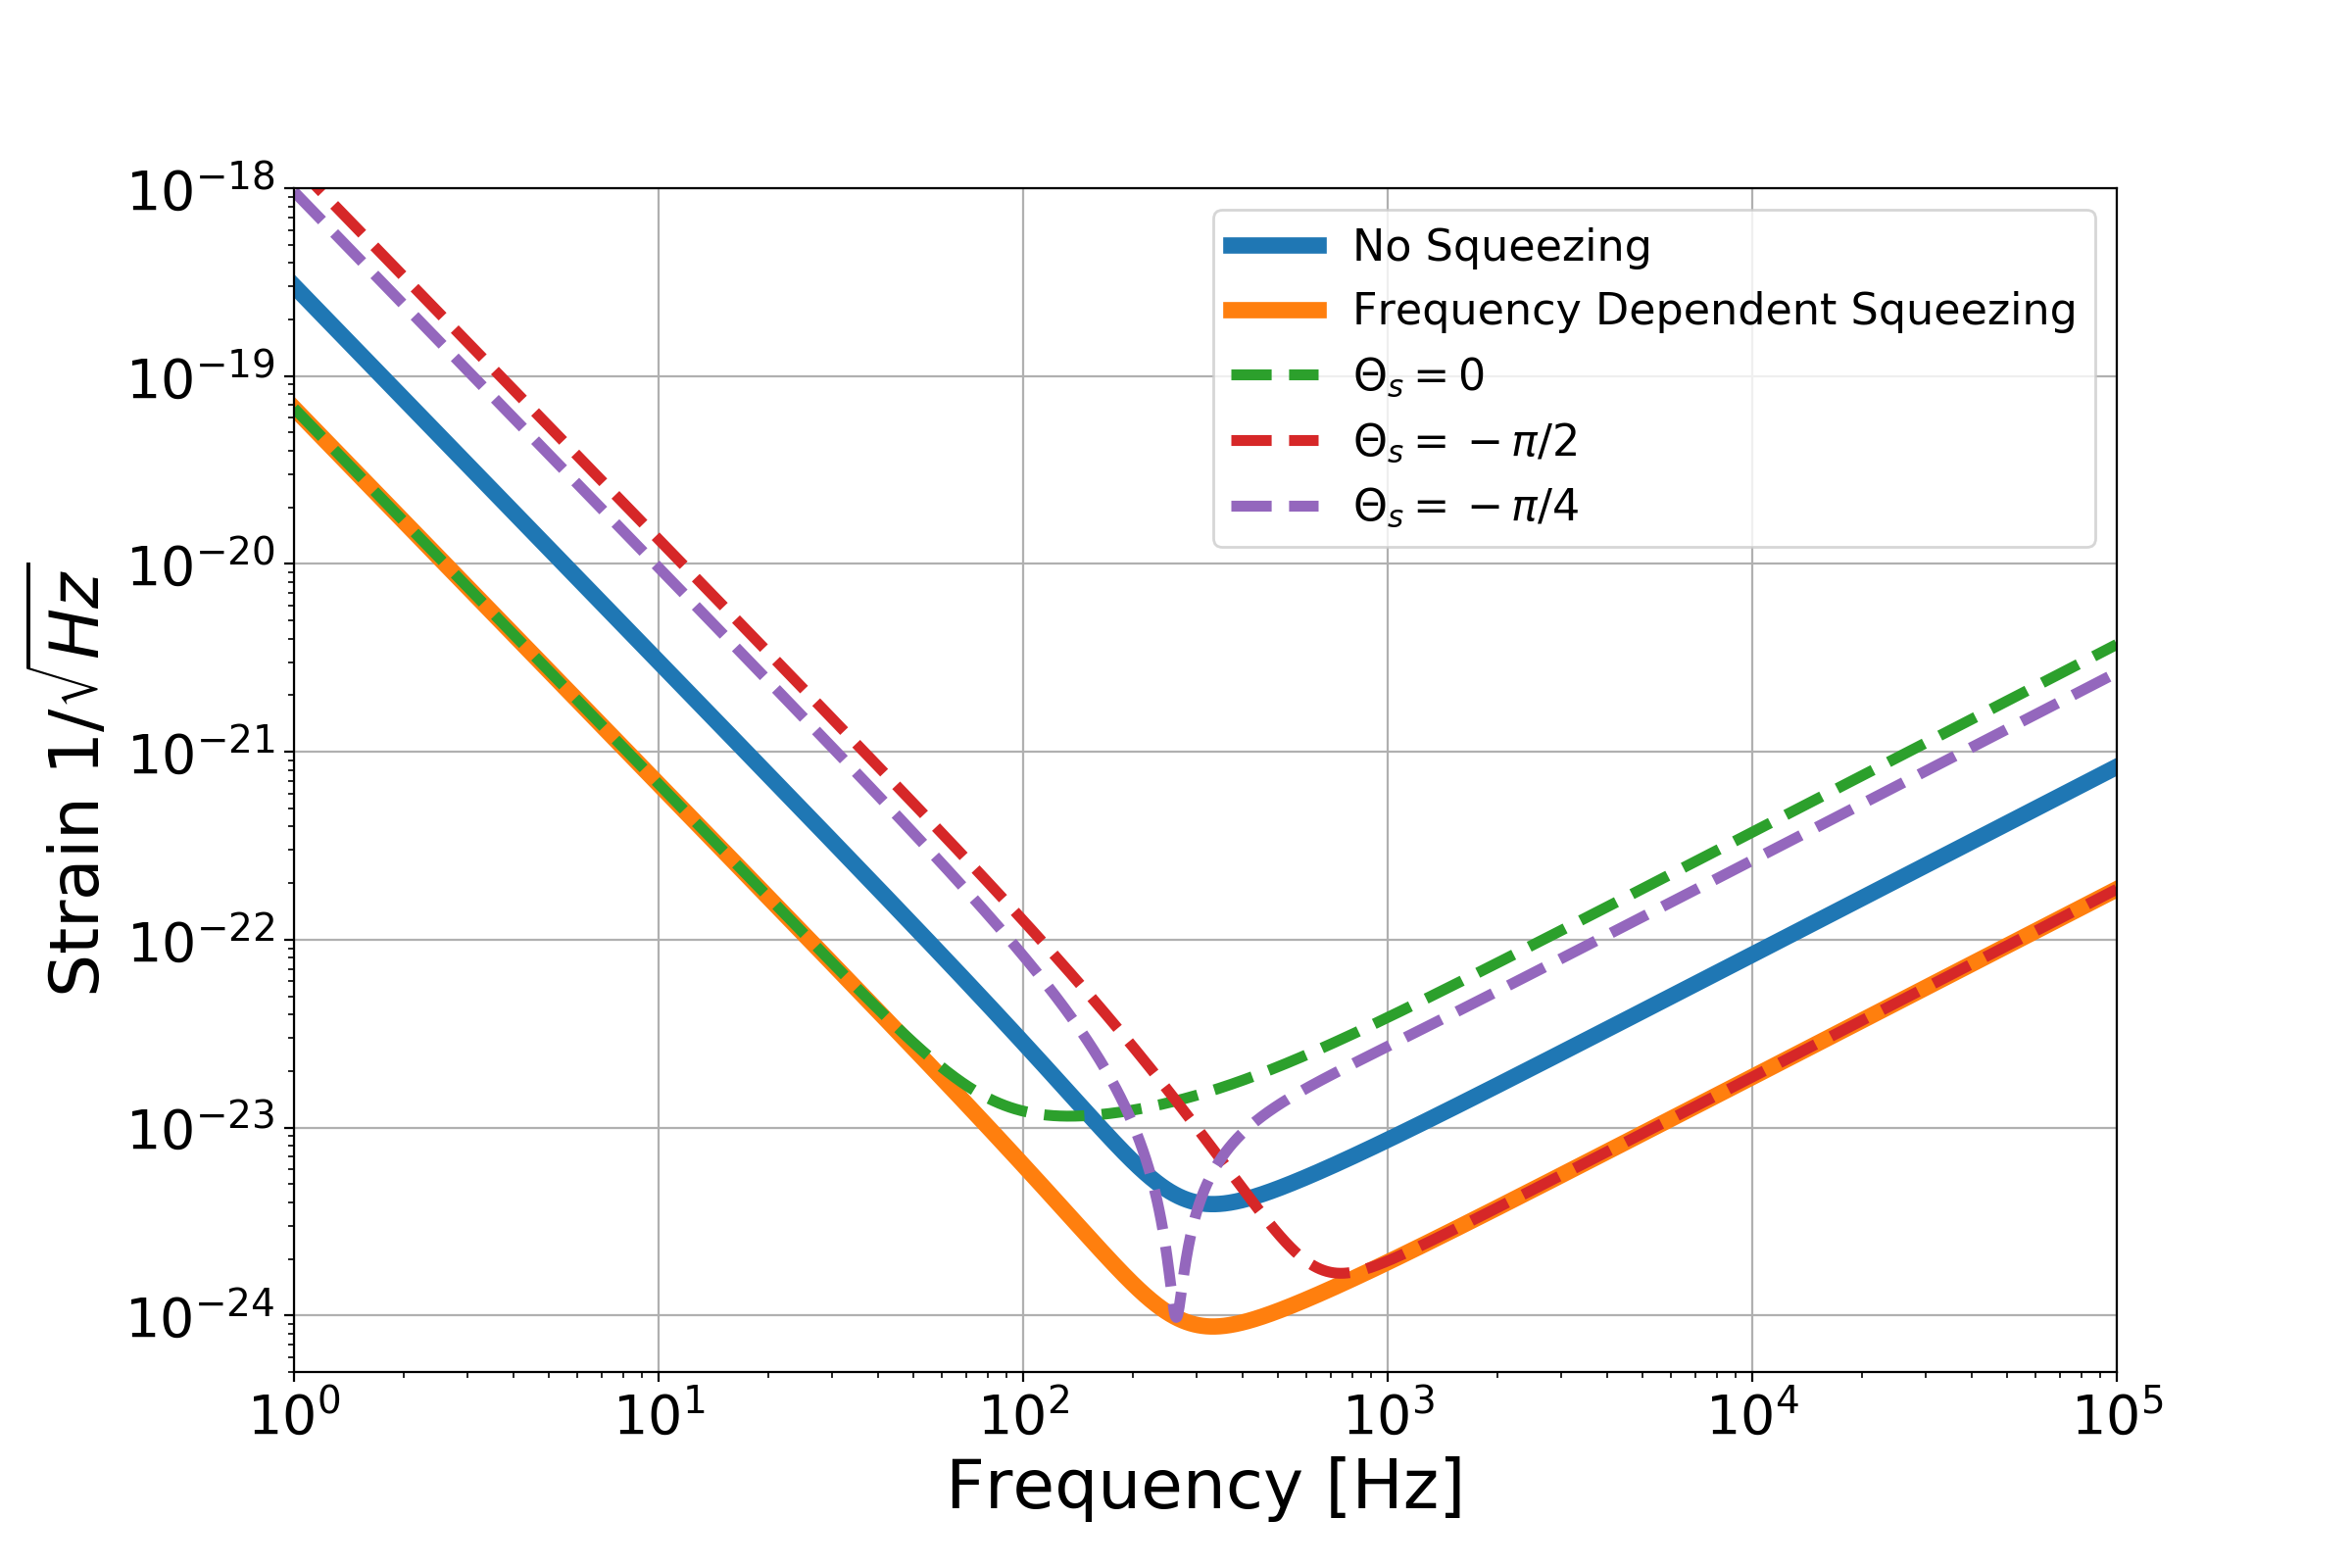
\includegraphics[width=\textwidth]{../Figures/Kimble_PRFPMI_QM_Sqz.png}
			\caption{Power recycled Fabry Perot Michelson quantum noise with various squeezing angles}
			\label{fig:kimble_PRFMI_sqz}
		\end{subfigure}
		\caption{Add a caption}
		\label{fig:PSD_PRFPMI}
	\end{figure}